\chapter{Obiekt symulowany - część projektowa}
Pierwszym etapem naszej pracy była analiza dostarczonego przez prowadzącego programu symulującego działanie obiektu. Był to obiekt dyskretny z opóźnieniem zależny od zmiennych procesu $U(k-11)$, $U(k-10)$, $Y(k-1)$, $Y(k-2)$.

Program do obsługi całego zadania symulacji został zaimplementowany w pliku \texttt{Projekt1.m}. Wykonywane są w nim wszystkie wymagane polecenia niezbędne do wykonania zadania, tj. sprawdzenie poprawności wartości w punkcie pracy $U_{\mathrm{pp}}$ i $Y_{\mathrm{pp}}$, wyznaczenie odpowiedzi skokowych procesu, wywołanie funkcji implementujących algorytmy PID i DMC, a także optymalizacja wskaźnika jakości regulacji $E$.

\section{Wyznaczenie odpowiedzi skokowych procesu}
Rozpoczynając od punktu pracy $U_{\mathrm{pp}}=\num{0,8}$ i $Y_{\mathrm{pp}}=2$ wyznaczaliśmy różne odpowiedzi skokowe dla kilku zmian sygnału sterującego. Wyniki symulacji przedstawione są na Rys.~\ref{os}. Jak widać, symulowany obiekt jest stabilny (charakterystyki po pewnym czasie ustalają się na stałym poziomie) oraz liniowy (charakterystyki statyczne $Y(U)$ leżą w przybliżeniu na linii prostej, co przedstawione jest na Rys.~\ref{cs}).

Na podstawie tej charakterystyki możemy obliczyć wzmocnienie statyczne procesu. Definiuje się je jako
\begin{equation}
K=\frac{\Delta Y}{\Delta U}
\end{equation}
Parametry $\Delta Y$ i $\Delta U$ są stałe dla dowolnie wybranych punktów na wykresie $Y(U)$, ponieważ charakterystyka jest liniowa. Należy więc wybrać dowolne punkty $(U_i, Y_i)$ i $(U_j, Y_j)$ i na ich podstawie obliczyć wzmocnienie statyczne $K$. Wynik:
\begin{equation}
K=1
\end{equation}

\begin{figure}
\centering
\caption{Odpowiedzi skokowe dla procesu symulowanego}
% This file was created by matlab2tikz.
%
\definecolor{mycolor1}{rgb}{1.00000,0.00000,1.00000}%
\definecolor{mycolor2}{rgb}{0.00000,1.00000,1.00000}%
%
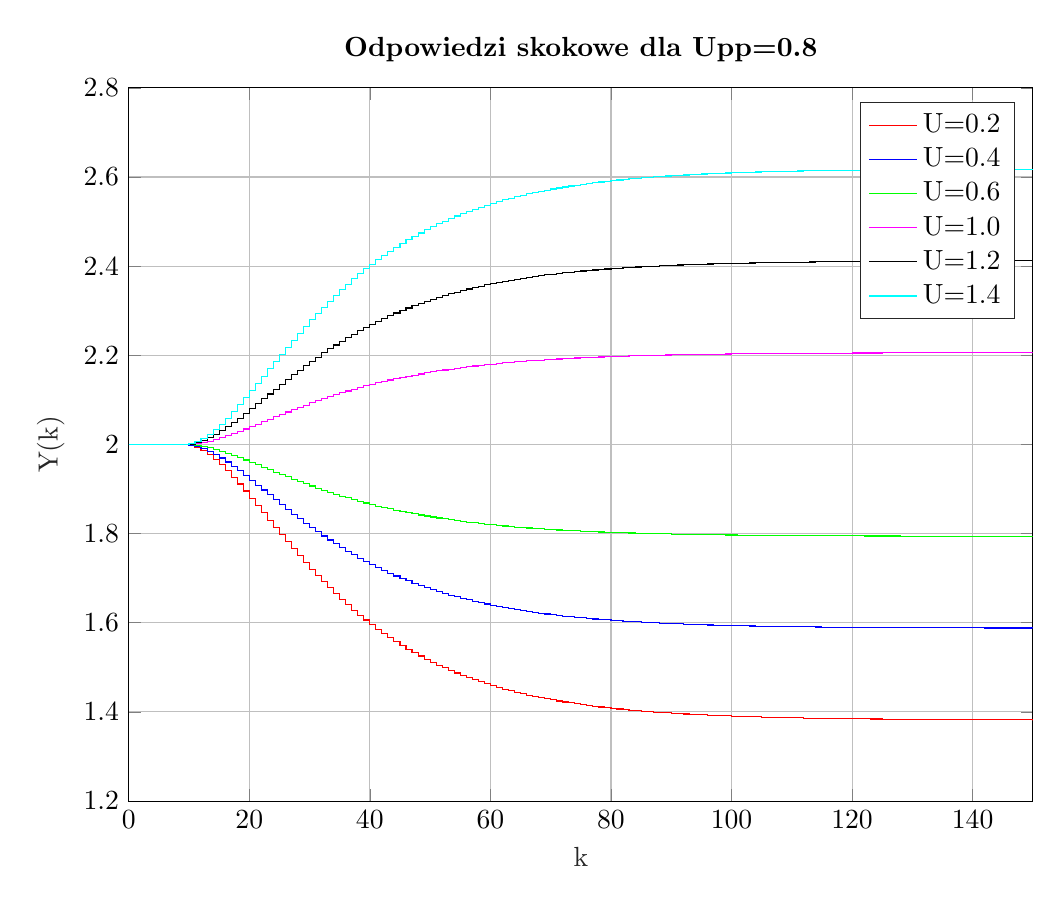
\begin{tikzpicture}

\begin{axis}[%
width=4.521in,
height=3.566in,
at={(0.758in,0.481in)},
scale only axis,
xmin=0,
xmax=150,
xlabel style={font=\color{white!15!black}},
xlabel={k},
ymin=1.2,
ymax=2.8,
ylabel style={font=\color{white!15!black}},
ylabel={Y(k)},
axis background/.style={fill=white},
title style={font=\bfseries},
title={Odpowiedzi skokowe dla Upp=0.8},
xmajorgrids,
ymajorgrids,
legend style={legend cell align=left, align=left, draw=white!15!black}
]
\addplot[const plot, color=red] table[row sep=crcr] {%
0	2\\
1	2\\
2	2\\
3	2\\
4	2\\
5	2\\
6	2\\
7	2\\
8	2\\
9	2\\
10	1.99836974\\
11	1.993804574792\\
12	1.98675077176943\\
13	1.9776031006434\\
14	1.96671022308248\\
15	1.95437954291634\\
16	1.94088156968435\\
17	1.92645384320798\\
18	1.9113044622537\\
19	1.89561525618372\\
20	1.87954463472339\\
21	1.86323014756816\\
22	1.84679078247401\\
23	1.83032902769341\\
24	1.81393272210415\\
25	1.79767671410647\\
26	1.78162434831043\\
27	1.76582879718065\\
28	1.75033425312912\\
29	1.73517699503257\\
30	1.72038634178294\\
31	1.70598550424369\\
32	1.69199234586852\\
33	1.67842006123113\\
34	1.66527778080386\\
35	1.65257110950162\\
36	1.64030260576434\\
37	1.62847220728182\\
38	1.61707760885926\\
39	1.60611459737593\\
40	1.59557734829637\\
41	1.58545868774896\\
42	1.57575032378499\\
43	1.56644305006941\\
44	1.55752692492794\\
45	1.54899142838022\\
46	1.5408255995233\\
47	1.53301815638995\\
48	1.52555760019054\\
49	1.51843230565225\\
50	1.51163059899408\\
51	1.50514082491827\\
52	1.49895140385573\\
53	1.49305088057565\\
54	1.48742796515313\\
55	1.4820715671855\\
56	1.47697082405375\\
57	1.47211512394192\\
58	1.46749412425114\\
59	1.46309776597717\\
60	1.45891628455902\\
61	1.45494021765133\\
62	1.45116041022364\\
63	1.44756801734544\\
64	1.44415450497611\\
65	1.44091164904313\\
66	1.43783153305977\\
67	1.43490654450505\\
68	1.43212937016277\\
69	1.42949299059359\\
70	1.42699067389351\\
71	1.42461596887342\\
72	1.42236269777852\\
73	1.42022494865097\\
74	1.41819706742667\\
75	1.41627364984496\\
76	1.41444953323988\\
77	1.41271978827207\\
78	1.4110797106526\\
79	1.40952481290224\\
80	1.40805081618348\\
81	1.40665364223685\\
82	1.40532940544786\\
83	1.4040744050667\\
84	1.4028851175984\\
85	1.40175818937833\\
86	1.40069042934424\\
87	1.39967880201383\\
88	1.39872042067429\\
89	1.39781254078826\\
90	1.39695255361896\\
91	1.39613798007566\\
92	1.39536646477943\\
93	1.3946357703478\\
94	1.39394377189641\\
95	1.39328845175437\\
96	1.39266789438998\\
97	1.39208028154234\\
98	1.39152388755441\\
99	1.39099707490234\\
100	1.39049828991594\\
101	1.39002605868451\\
102	1.38957898314264\\
103	1.38915573732998\\
104	1.38875506381921\\
105	1.38837577030638\\
106	1.38801672635763\\
107	1.38767686030665\\
108	1.38735515629701\\
109	1.38705065146363\\
110	1.38676243324802\\
111	1.38648963684166\\
112	1.38623144275223\\
113	1.38598707448758\\
114	1.38575579635226\\
115	1.38553691135188\\
116	1.38532975920029\\
117	1.38513371442538\\
118	1.38494818456859\\
119	1.38477260847429\\
120	1.38460645466458\\
121	1.38444921979572\\
122	1.38430042719231\\
123	1.38415962545559\\
124	1.38402638714221\\
125	1.38390030751035\\
126	1.38378100332965\\
127	1.38366811175211\\
128	1.38356128924083\\
129	1.38346021055382\\
130	1.38336456778021\\
131	1.38327406942618\\
132	1.38318843954819\\
133	1.38310741693113\\
134	1.38303075430927\\
135	1.38295821762756\\
136	1.38288958534161\\
137	1.38282464775412\\
138	1.38276320638603\\
139	1.3827050733806\\
140	1.38265007093876\\
141	1.38259803078406\\
142	1.38254879365582\\
143	1.38250220882889\\
144	1.38245813365874\\
145	1.38241643315059\\
146	1.38237697955126\\
147	1.38233965196255\\
148	1.38230433597519\\
149	1.38227092332205\\
150	1.38223931154985\\
};
\addlegendentry{U=0.2}

\addplot[const plot, color=blue] table[row sep=crcr] {%
0	2\\
1	2\\
2	2\\
3	2\\
4	2\\
5	2\\
6	2\\
7	2\\
8	2\\
9	2\\
10	1.99891316\\
11	1.995869716528\\
12	1.99116718117962\\
13	1.98506873376227\\
14	1.97780681538832\\
15	1.96958636194423\\
16	1.9605877131229\\
17	1.95096922880532\\
18	1.94086964150247\\
19	1.93041017078914\\
20	1.91969642314893\\
21	1.90882009837877\\
22	1.89786052164934\\
23	1.88688601846227\\
24	1.87595514806944\\
25	1.86511780940432\\
26	1.85441623220696\\
27	1.8438858647871\\
28	1.83355616875275\\
29	1.82345133002171\\
30	1.81359089452196\\
31	1.80399033616246\\
32	1.79466156391235\\
33	1.78561337415408\\
34	1.77685185386924\\
35	1.76838073966775\\
36	1.76020173717623\\
37	1.75231480485455\\
38	1.74471840590618\\
39	1.73740973158395\\
40	1.73038489886425\\
41	1.72363912516598\\
42	1.71716688252333\\
43	1.71096203337961\\
44	1.70501794995197\\
45	1.69932761892015\\
46	1.69388373301554\\
47	1.68867877092664\\
48	1.6837050667937\\
49	1.67895487043484\\
50	1.67442039932939\\
51	1.67009388327885\\
52	1.66596760257049\\
53	1.66203392038377\\
54	1.65828531010209\\
55	1.65471437812367\\
56	1.6513138827025\\
57	1.64807674929462\\
58	1.6449960828341\\
59	1.64206517731812\\
60	1.63927752303935\\
61	1.63662681176756\\
62	1.6341069401491\\
63	1.63171201156363\\
64	1.62943633665074\\
65	1.62727443269542\\
66	1.62522102203985\\
67	1.62327102967004\\
68	1.62141958010851\\
69	1.61966199372906\\
70	1.61799378259567\\
71	1.61641064591562\\
72	1.61490846518568\\
73	1.61348329910065\\
74	1.61213137828445\\
75	1.61084909989664\\
76	1.60963302215992\\
77	1.60847985884805\\
78	1.6073864737684\\
79	1.60634987526816\\
80	1.60536721078899\\
81	1.60443576149123\\
82	1.60355293696524\\
83	1.60271627004447\\
84	1.60192341173227\\
85	1.60117212625222\\
86	1.60046028622949\\
87	1.59978586800922\\
88	1.59914694711619\\
89	1.59854169385884\\
90	1.5979683690793\\
91	1.59742532005044\\
92	1.59691097651962\\
93	1.59642384689853\\
94	1.5959625145976\\
95	1.59552563450291\\
96	1.59511192959332\\
97	1.59472018769489\\
98	1.5943492583696\\
99	1.59399804993489\\
100	1.59366552661062\\
101	1.59335070578967\\
102	1.59305265542842\\
103	1.59277049155331\\
104	1.59250337587947\\
105	1.59225051353758\\
106	1.59201115090508\\
107	1.59178457353776\\
108	1.591570104198\\
109	1.59136710097574\\
110	1.59117495549867\\
111	1.59099309122776\\
112	1.59082096183481\\
113	1.59065804965838\\
114	1.59050386423484\\
115	1.59035794090124\\
116	1.59021983946686\\
117	1.59008914295025\\
118	1.58996545637906\\
119	1.58984840564952\\
120	1.58973763644305\\
121	1.58963281319714\\
122	1.5895336181282\\
123	1.58943975030372\\
124	1.58935092476147\\
125	1.58926687167356\\
126	1.5891873355531\\
127	1.5891120745014\\
128	1.58904085949388\\
129	1.58897347370254\\
130	1.58890971185347\\
131	1.58884937961745\\
132	1.58879229303212\\
133	1.58873827795408\\
134	1.58868716953951\\
135	1.5886388117517\\
136	1.5885930568944\\
137	1.58854976516941\\
138	1.58850880425735\\
139	1.5884700489204\\
140	1.58843338062584\\
141	1.58839868718937\\
142	1.58836586243721\\
143	1.58833480588592\\
144	1.58830542243915\\
145	1.58827762210039\\
146	1.58825131970084\\
147	1.5882264346417\\
148	1.58820289065012\\
149	1.58818061554803\\
150	1.58815954103323\\
};
\addlegendentry{U=0.4}

\addplot[const plot, color=green] table[row sep=crcr] {%
0	2\\
1	2\\
2	2\\
3	2\\
4	2\\
5	2\\
6	2\\
7	2\\
8	2\\
9	2\\
10	1.99945658\\
11	1.997934858264\\
12	1.99558359058981\\
13	1.99253436688113\\
14	1.98890340769416\\
15	1.98479318097211\\
16	1.98029385656145\\
17	1.97548461440266\\
18	1.97043482075123\\
19	1.96520508539457\\
20	1.95984821157446\\
21	1.95441004918939\\
22	1.94893026082467\\
23	1.94344300923114\\
24	1.93797757403472\\
25	1.93255890470216\\
26	1.92720811610348\\
27	1.92194293239355\\
28	1.91677808437637\\
29	1.91172566501086\\
30	1.90679544726098\\
31	1.90199516808123\\
32	1.89733078195617\\
33	1.89280668707704\\
34	1.88842592693462\\
35	1.88419036983387\\
36	1.88010086858811\\
37	1.87615740242727\\
38	1.87235920295309\\
39	1.86870486579198\\
40	1.86519244943212\\
41	1.86181956258299\\
42	1.85858344126167\\
43	1.85548101668981\\
44	1.85250897497598\\
45	1.84966380946008\\
46	1.84694186650777\\
47	1.84433938546332\\
48	1.84185253339685\\
49	1.83947743521742\\
50	1.8372101996647\\
51	1.83504694163943\\
52	1.83298380128525\\
53	1.83101696019189\\
54	1.82914265505105\\
55	1.82735718906184\\
56	1.82565694135125\\
57	1.82403837464731\\
58	1.82249804141705\\
59	1.82103258865906\\
60	1.81963876151968\\
61	1.81831340588378\\
62	1.81705347007455\\
63	1.81585600578182\\
64	1.81471816832537\\
65	1.81363721634771\\
66	1.81261051101993\\
67	1.81163551483502\\
68	1.81070979005426\\
69	1.80983099686453\\
70	1.80899689129784\\
71	1.80820532295781\\
72	1.80745423259284\\
73	1.80674164955033\\
74	1.80606568914223\\
75	1.80542454994832\\
76	1.80481651107996\\
77	1.80423992942403\\
78	1.8036932368842\\
79	1.80317493763408\\
80	1.8026836053945\\
81	1.80221788074562\\
82	1.80177646848262\\
83	1.80135813502224\\
84	1.80096170586614\\
85	1.80058606312611\\
86	1.80023014311475\\
87	1.79989293400461\\
88	1.7995734735581\\
89	1.79927084692942\\
90	1.79898418453966\\
91	1.79871266002522\\
92	1.79845548825981\\
93	1.79821192344927\\
94	1.79798125729881\\
95	1.79776281725146\\
96	1.79755596479666\\
97	1.79736009384745\\
98	1.7971746291848\\
99	1.79699902496745\\
100	1.79683276330531\\
101	1.79667535289484\\
102	1.79652632771421\\
103	1.79638524577666\\
104	1.79625168793974\\
105	1.79612525676879\\
106	1.79600557545254\\
107	1.79589228676888\\
108	1.795785052099\\
109	1.79568355048787\\
110	1.79558747774934\\
111	1.79549654561388\\
112	1.79541048091741\\
113	1.79532902482919\\
114	1.79525193211742\\
115	1.79517897045062\\
116	1.79510991973343\\
117	1.79504457147512\\
118	1.79498272818953\\
119	1.79492420282476\\
120	1.79486881822152\\
121	1.79481640659857\\
122	1.7947668090641\\
123	1.79471987515186\\
124	1.79467546238074\\
125	1.79463343583678\\
126	1.79459366777655\\
127	1.7945560372507\\
128	1.79452042974694\\
129	1.79448673685127\\
130	1.79445485592674\\
131	1.79442468980873\\
132	1.79439614651606\\
133	1.79436913897704\\
134	1.79434358476976\\
135	1.79431940587585\\
136	1.7942965284472\\
137	1.79427488258471\\
138	1.79425440212868\\
139	1.7942350244602\\
140	1.79421669031292\\
141	1.79419934359469\\
142	1.79418293121861\\
143	1.79416740294296\\
144	1.79415271121958\\
145	1.7941388110502\\
146	1.79412565985042\\
147	1.79411321732085\\
148	1.79410144532506\\
149	1.79409030777402\\
150	1.79407977051661\\
};
\addlegendentry{U=0.6}

\addplot[const plot, color=mycolor1] table[row sep=crcr] {%
0	2\\
1	2\\
2	2\\
3	2\\
4	2\\
5	2\\
6	2\\
7	2\\
8	2\\
9	2\\
10	2.00054342\\
11	2.002065141736\\
12	2.00441640941019\\
13	2.00746563311887\\
14	2.01109659230584\\
15	2.01520681902789\\
16	2.01970614343855\\
17	2.02451538559734\\
18	2.02956517924877\\
19	2.03479491460543\\
20	2.04015178842554\\
21	2.04558995081062\\
22	2.05106973917533\\
23	2.05655699076887\\
24	2.06202242596528\\
25	2.06744109529784\\
26	2.07279188389652\\
27	2.07805706760645\\
28	2.08322191562363\\
29	2.08827433498915\\
30	2.09320455273902\\
31	2.09800483191877\\
32	2.10266921804382\\
33	2.10719331292296\\
34	2.11157407306538\\
35	2.11580963016613\\
36	2.11989913141189\\
37	2.12384259757272\\
38	2.12764079704691\\
39	2.13129513420802\\
40	2.13480755056787\\
41	2.13818043741701\\
42	2.14141655873833\\
43	2.14451898331019\\
44	2.14749102502402\\
45	2.15033619053992\\
46	2.15305813349223\\
47	2.15566061453668\\
48	2.15814746660315\\
49	2.16052256478258\\
50	2.1627898003353\\
51	2.16495305836057\\
52	2.16701619871475\\
53	2.16898303980811\\
54	2.17085734494895\\
55	2.17264281093816\\
56	2.17434305864875\\
57	2.17596162535269\\
58	2.17750195858295\\
59	2.17896741134094\\
60	2.18036123848032\\
61	2.18168659411622\\
62	2.18294652992545\\
63	2.18414399421819\\
64	2.18528183167463\\
65	2.18636278365229\\
66	2.18738948898008\\
67	2.18836448516498\\
68	2.18929020994574\\
69	2.19016900313547\\
70	2.19100310870216\\
71	2.19179467704219\\
72	2.19254576740716\\
73	2.19325835044968\\
74	2.19393431085778\\
75	2.19457545005168\\
76	2.19518348892004\\
77	2.19576007057598\\
78	2.1963067631158\\
79	2.19682506236592\\
80	2.19731639460551\\
81	2.19778211925439\\
82	2.19822353151738\\
83	2.19864186497777\\
84	2.19903829413387\\
85	2.19941393687389\\
86	2.19976985688525\\
87	2.20010706599539\\
88	2.2004265264419\\
89	2.20072915307058\\
90	2.20101581546035\\
91	2.20128733997478\\
92	2.20154451174019\\
93	2.20178807655074\\
94	2.2020187427012\\
95	2.20223718274855\\
96	2.20244403520334\\
97	2.20263990615256\\
98	2.2028253708152\\
99	2.20300097503256\\
100	2.20316723669469\\
101	2.20332464710517\\
102	2.20347367228579\\
103	2.20361475422334\\
104	2.20374831206026\\
105	2.20387474323121\\
106	2.20399442454746\\
107	2.20410771323112\\
108	2.204214947901\\
109	2.20431644951213\\
110	2.20441252225066\\
111	2.20450345438612\\
112	2.20458951908259\\
113	2.20467097517081\\
114	2.20474806788258\\
115	2.20482102954937\\
116	2.20489008026657\\
117	2.20495542852487\\
118	2.20501727181047\\
119	2.20507579717524\\
120	2.20513118177847\\
121	2.20518359340143\\
122	2.20523319093589\\
123	2.20528012484814\\
124	2.20532453761926\\
125	2.20536656416321\\
126	2.20540633222345\\
127	2.20544396274929\\
128	2.20547957025305\\
129	2.20551326314872\\
130	2.20554514407326\\
131	2.20557531019127\\
132	2.20560385348394\\
133	2.20563086102295\\
134	2.20565641523024\\
135	2.20568059412414\\
136	2.20570347155279\\
137	2.20572511741529\\
138	2.20574559787132\\
139	2.2057649755398\\
140	2.20578330968708\\
141	2.20580065640531\\
142	2.20581706878139\\
143	2.20583259705704\\
144	2.20584728878042\\
145	2.2058611889498\\
146	2.20587434014958\\
147	2.20588678267915\\
148	2.20589855467494\\
149	2.20590969222599\\
150	2.20592022948339\\
};
\addlegendentry{U=1.0}

\addplot[const plot, color=black] table[row sep=crcr] {%
0	2\\
1	2\\
2	2\\
3	2\\
4	2\\
5	2\\
6	2\\
7	2\\
8	2\\
9	2\\
10	2.00108684\\
11	2.004130283472\\
12	2.00883281882038\\
13	2.01493126623773\\
14	2.02219318461168\\
15	2.03041363805577\\
16	2.0394122868771\\
17	2.04903077119468\\
18	2.05913035849753\\
19	2.06958982921086\\
20	2.08030357685107\\
21	2.09117990162123\\
22	2.10213947835066\\
23	2.11311398153773\\
24	2.12404485193056\\
25	2.13488219059568\\
26	2.14558376779304\\
27	2.1561141352129\\
28	2.16644383124725\\
29	2.17654866997829\\
30	2.18640910547804\\
31	2.19600966383754\\
32	2.20533843608765\\
33	2.21438662584592\\
34	2.22314814613076\\
35	2.23161926033225\\
36	2.23979826282377\\
37	2.24768519514545\\
38	2.25528159409382\\
39	2.26259026841605\\
40	2.26961510113575\\
41	2.27636087483402\\
42	2.28283311747667\\
43	2.28903796662039\\
44	2.29498205004803\\
45	2.30067238107984\\
46	2.30611626698446\\
47	2.31132122907336\\
48	2.3162949332063\\
49	2.32104512956516\\
50	2.32557960067061\\
51	2.32990611672115\\
52	2.33403239742951\\
53	2.33796607961623\\
54	2.34171468989791\\
55	2.34528562187633\\
56	2.3486861172975\\
57	2.35192325070538\\
58	2.3550039171659\\
59	2.35793482268188\\
60	2.36072247696065\\
61	2.36337318823244\\
62	2.3658930598509\\
63	2.36828798843637\\
64	2.37056366334926\\
65	2.37272556730458\\
66	2.37477897796015\\
67	2.37672897032996\\
68	2.37858041989148\\
69	2.38033800627093\\
70	2.38200621740432\\
71	2.38358935408438\\
72	2.38509153481431\\
73	2.38651670089935\\
74	2.38786862171555\\
75	2.38915090010335\\
76	2.39036697784007\\
77	2.39152014115195\\
78	2.39261352623159\\
79	2.39365012473183\\
80	2.394632789211\\
81	2.39556423850876\\
82	2.39644706303475\\
83	2.39728372995553\\
84	2.39807658826773\\
85	2.39882787374777\\
86	2.3995397137705\\
87	2.40021413199077\\
88	2.4008530528838\\
89	2.40145830614115\\
90	2.40203163092069\\
91	2.40257467994955\\
92	2.40308902348038\\
93	2.40357615310146\\
94	2.40403748540239\\
95	2.40447436549708\\
96	2.40488807040667\\
97	2.4052798123051\\
98	2.40565074163039\\
99	2.4060019500651\\
100	2.40633447338937\\
101	2.40664929421033\\
102	2.40694734457157\\
103	2.40722950844668\\
104	2.40749662412053\\
105	2.40774948646242\\
106	2.40798884909492\\
107	2.40821542646223\\
108	2.408429895802\\
109	2.40863289902425\\
110	2.40882504450133\\
111	2.40900690877224\\
112	2.40917903816519\\
113	2.40934195034162\\
114	2.40949613576516\\
115	2.40964205909876\\
116	2.40978016053314\\
117	2.40991085704975\\
118	2.41003454362094\\
119	2.41015159435048\\
120	2.41026236355695\\
121	2.41036718680286\\
122	2.4104663818718\\
123	2.41056024969628\\
124	2.41064907523853\\
125	2.41073312832644\\
126	2.4108126644469\\
127	2.4108879254986\\
128	2.41095914050612\\
129	2.41102652629746\\
130	2.41109028814653\\
131	2.41115062038255\\
132	2.41120770696788\\
133	2.41126172204591\\
134	2.41131283046049\\
135	2.41136118824829\\
136	2.41140694310559\\
137	2.41145023483059\\
138	2.41149119574265\\
139	2.4115299510796\\
140	2.41156661937416\\
141	2.41160131281063\\
142	2.41163413756279\\
143	2.41166519411408\\
144	2.41169457756084\\
145	2.41172237789961\\
146	2.41174868029916\\
147	2.4117735653583\\
148	2.41179710934988\\
149	2.41181938445197\\
150	2.41184045896677\\
};
\addlegendentry{U=1.2}

\addplot[const plot, color=mycolor2] table[row sep=crcr] {%
0	2\\
1	2\\
2	2\\
3	2\\
4	2\\
5	2\\
6	2\\
7	2\\
8	2\\
9	2\\
10	2.00163026\\
11	2.006195425208\\
12	2.01324922823057\\
13	2.0223968993566\\
14	2.03328977691752\\
15	2.04562045708366\\
16	2.05911843031565\\
17	2.07354615679203\\
18	2.0886955377463\\
19	2.10438474381629\\
20	2.12045536527662\\
21	2.13676985243185\\
22	2.153209217526\\
23	2.1696709723066\\
24	2.18606727789585\\
25	2.20232328589353\\
26	2.21837565168957\\
27	2.23417120281935\\
28	2.24966574687089\\
29	2.26482300496744\\
30	2.27961365821707\\
31	2.29401449575632\\
32	2.30800765413148\\
33	2.32157993876888\\
34	2.33472221919614\\
35	2.34742889049839\\
36	2.35969739423567\\
37	2.37152779271819\\
38	2.38292239114074\\
39	2.39388540262408\\
40	2.40442265170364\\
41	2.41454131225104\\
42	2.42424967621501\\
43	2.43355694993059\\
44	2.44247307507206\\
45	2.45100857161978\\
46	2.4591744004767\\
47	2.46698184361005\\
48	2.47444239980946\\
49	2.48156769434775\\
50	2.48836940100592\\
51	2.49485917508173\\
52	2.50104859614427\\
53	2.50694911942435\\
54	2.51257203484687\\
55	2.5179284328145\\
56	2.52302917594625\\
57	2.52788487605808\\
58	2.53250587574885\\
59	2.53690223402283\\
60	2.54108371544098\\
61	2.54505978234866\\
62	2.54883958977635\\
63	2.55243198265456\\
64	2.55584549502389\\
65	2.55908835095687\\
66	2.56216846694022\\
67	2.56509345549495\\
68	2.56787062983723\\
69	2.5705070094064\\
70	2.57300932610649\\
71	2.57538403112657\\
72	2.57763730222147\\
73	2.57977505134902\\
74	2.58180293257333\\
75	2.58372635015503\\
76	2.58555046676011\\
77	2.58728021172792\\
78	2.58892028934739\\
79	2.59047518709775\\
80	2.59194918381651\\
81	2.59334635776315\\
82	2.59467059455213\\
83	2.5959255949333\\
84	2.59711488240159\\
85	2.59824181062166\\
86	2.59930957065575\\
87	2.60032119798616\\
88	2.6012795793257\\
89	2.60218745921174\\
90	2.60304744638104\\
91	2.60386201992433\\
92	2.60463353522057\\
93	2.6053642296522\\
94	2.60605622810359\\
95	2.60671154824563\\
96	2.60733210561002\\
97	2.60791971845766\\
98	2.60847611244559\\
99	2.60900292509766\\
100	2.60950171008406\\
101	2.6099739413155\\
102	2.61042101685737\\
103	2.61084426267003\\
104	2.61124493618079\\
105	2.61162422969363\\
106	2.61198327364238\\
107	2.61232313969335\\
108	2.612644843703\\
109	2.61294934853638\\
110	2.61323756675199\\
111	2.61351036315835\\
112	2.61376855724777\\
113	2.61401292551243\\
114	2.61424420364774\\
115	2.61446308864813\\
116	2.61467024079971\\
117	2.61486628557462\\
118	2.61505181543141\\
119	2.61522739152571\\
120	2.61539354533542\\
121	2.61555078020428\\
122	2.61569957280768\\
123	2.61584037454441\\
124	2.61597361285778\\
125	2.61609969248964\\
126	2.61621899667034\\
127	2.61633188824788\\
128	2.61643871075917\\
129	2.61653978944618\\
130	2.61663543221978\\
131	2.61672593057381\\
132	2.61681156045181\\
133	2.61689258306886\\
134	2.61696924569072\\
135	2.61704178237243\\
136	2.61711041465838\\
137	2.61717535224587\\
138	2.61723679361396\\
139	2.61729492661939\\
140	2.61734992906123\\
141	2.61740196921593\\
142	2.61745120634417\\
143	2.61749779117111\\
144	2.61754186634126\\
145	2.6175835668494\\
146	2.61762302044874\\
147	2.61766034803744\\
148	2.61769566402481\\
149	2.61772907667795\\
150	2.61776068845015\\
};
\addlegendentry{U=1.4}

\end{axis}
\end{tikzpicture}%
\label{os}
\end{figure}

\begin{figure}
\centering
\caption{Charakterystyka statyczna}
% This file was created by matlab2tikz.
%
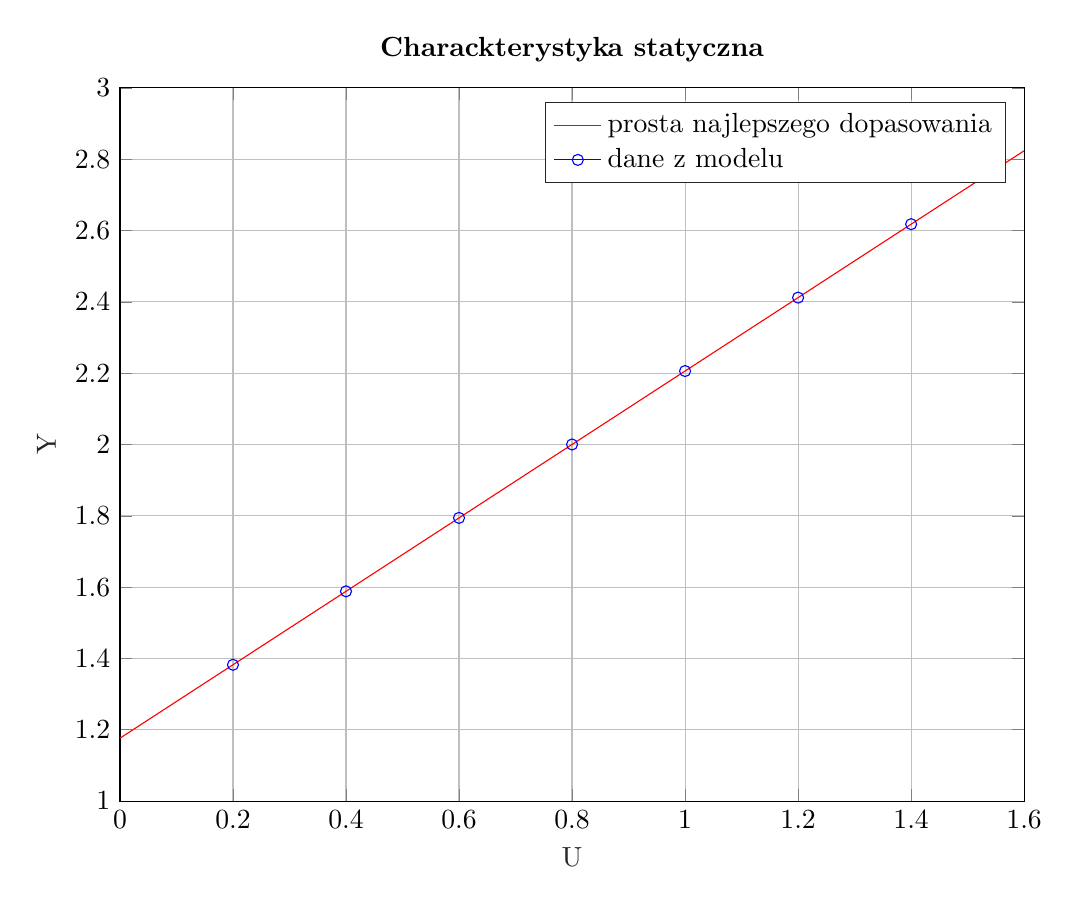
\begin{tikzpicture}

\begin{axis}[%
width=4.521in,
height=3.566in,
at={(0.758in,0.481in)},
scale only axis,
xmin=0,
xmax=1.6,
xlabel style={font=\color{white!15!black}},
xlabel={U},
ymin=1,
ymax=3,
ylabel style={font=\color{white!15!black}},
ylabel={Y},
axis background/.style={fill=white},
title style={font=\bfseries},
title={Charackterystyka statyczna},
xmajorgrids,
ymajorgrids,
legend style={legend cell align=left, align=left, draw=white!15!black}
]
\addplot [color=red]
  table[row sep=crcr]{%
0	1.17631908206646\\
0.1	1.27927919680815\\
0.2	1.38223931154984\\
0.3	1.48519942629154\\
0.4	1.58815954103323\\
0.5	1.69111965577492\\
0.6	1.79407977051661\\
0.7	1.89703988525831\\
0.8	2\\
0.9	2.10296011474169\\
1	2.20592022948338\\
1.1	2.30888034422508\\
1.2	2.41184045896677\\
1.3	2.51480057370846\\
1.4	2.61776068845015\\
1.5	2.72072080319185\\
1.6	2.82368091793354\\
};
\addlegendentry{prosta najlepszego dopasowania}

\addplot [color=blue, draw=none, mark=o, mark options={solid, blue}]
  table[row sep=crcr]{%
0.2	1.38223931154985\\
0.4	1.58815954103323\\
0.6	1.79407977051661\\
0.8	2\\
1	2.20592022948339\\
1.2	2.41184045896677\\
1.4	2.61776068845015\\
};
\addlegendentry{dane z modelu}

\end{axis}
\end{tikzpicture}%
\label{cs}
\end{figure}

Aby otrzymać odpowiedź skokową wykorzystywaną w algorytmie DMC należy pobudzić obiekt skokiem jednostkowym, gdzie od chwili zerowej sygnał sterujący ma wartość 1, a w przeszłości jest zerowy. Wynik tej odpowiedzi skokowej jest przedstawiony na Rys.~\ref{skok1}.

\begin{figure}

\centering
\caption{Odp. skokowa do algorytmu DMC}
% This file was created by matlab2tikz.
%
\begin{tikzpicture}

\begin{axis}[%
width=4.521in,
height=3.566in,
at={(0.758in,0.481in)},
scale only axis,
xmin=0,
xmax=150,
xlabel style={font=\color{white!15!black}},
xlabel={k},
ymin=0,
ymax=1.2,
ylabel style={font=\color{white!15!black}},
ylabel={Y(k)},
axis background/.style={fill=white},
title style={font=\bfseries},
title={Odpowied� skokowa dla DMC},
xmajorgrids,
ymajorgrids,
legend style={legend cell align=left, align=left, draw=white!15!black}
]
\addplot[const plot, color=red] table[row sep=crcr] {%
0	0\\
1	0\\
2	0\\
3	0\\
4	0\\
5	0\\
6	0\\
7	0\\
8	0\\
9	0\\
10	0.00271710000000036\\
11	0.0103257086800013\\
12	0.0220820470509464\\
13	0.0373281655943303\\
14	0.0554829615291985\\
15	0.07603409513943\\
16	0.0985307171927552\\
17	0.122576927986708\\
18	0.147825896243834\\
19	0.173974573027145\\
20	0.200758942127692\\
21	0.227949754053078\\
22	0.25534869587666\\
23	0.282784953844331\\
24	0.310112129826419\\
25	0.33720547648922\\
26	0.363959419482622\\
27	0.390285338032255\\
28	0.41610957811814\\
29	0.441371674945725\\
30	0.466022763695106\\
31	0.490024159593858\\
32	0.513346090219122\\
33	0.535966564614785\\
34	0.557870365326889\\
35	0.579048150830628\\
36	0.599495657059428\\
37	0.619212987863622\\
38	0.638203985234544\\
39	0.656475671040107\\
40	0.674037752839374\\
41	0.690902187085045\\
42	0.707082793691667\\
43	0.722594916550963\\
44	0.737455125120077\\
45	0.751680952699607\\
46	0.765290667461154\\
47	0.778303072683402\\
48	0.790737333015741\\
49	0.802612823912903\\
50	0.813949001676506\\
51	0.824765291802867\\
52	0.835080993573758\\
53	0.844915199040566\\
54	0.854286724744757\\
55	0.863214054690815\\
56	0.871715293243733\\
57	0.879808126763446\\
58	0.887509792914745\\
59	0.894837056704705\\
60	0.901806192401622\\
61	0.908432970581097\\
62	0.91473264962725\\
63	0.920719971090931\\
64	0.926409158373147\\
65	0.931813918261448\\
66	0.936947444900378\\
67	0.941822425824916\\
68	0.946451049728725\\
69	0.950845015677344\\
70	0.955015543510824\\
71	0.958973385210968\\
72	0.962728837035804\\
73	0.966291752248392\\
74	0.969671554288896\\
75	0.972877250258399\\
76	0.975917444600207\\
77	0.978800352879889\\
78	0.981533815578999\\
79	0.984125311829598\\
80	0.986581973027532\\
81	0.98891059627193\\
82	0.991117657586904\\
83	0.993209324888846\\
84	0.995191470669341\\
85	0.997069684369456\\
86	0.998849284426273\\
87	1.00053532997695\\
88	1.00213263220952\\
89	1.00364576535291\\
90	1.00507907730175\\
91	1.00643669987391\\
92	1.00772255870097\\
93	1.00894038275368\\
94	1.01009371350601\\
95	1.01118591374273\\
96	1.01222017601671\\
97	1.01319953076278\\
98	1.01412685407601\\
99	1.01500487516278\\
100	1.01583618347345\\
101	1.01662323552584\\
102	1.01736836142895\\
103	1.01807377111672\\
104	1.01874156030132\\
105	1.01937371615605\\
106	1.0199721227373\\
107	1.02053856615559\\
108	1.02107473950499\\
109	1.02158224756063\\
110	1.02206261125331\\
111	1.02251727193058\\
112	1.02294759541296\\
113	1.02335487585404\\
114	1.02374033941289\\
115	1.02410514774687\\
116	1.02445040133284\\
117	1.02477714262437\\
118	1.02508635905234\\
119	1.02537898587618\\
120	1.02565590889236\\
121	1.02591796700713\\
122	1.02616595467947\\
123	1.02640062424068\\
124	1.0266226880963\\
125	1.02683282081607\\
126	1.02703166111723\\
127	1.02721981374646\\
128	1.02739785126527\\
129	1.02756631574362\\
130	1.02772572036629\\
131	1.02787655095634\\
132	1.02801926741968\\
133	1.02815430511476\\
134	1.0282820761512\\
135	1.02840297062072\\
136	1.02851735776397\\
137	1.02862558707645\\
138	1.0287279893566\\
139	1.02882487769898\\
140	1.02891654843539\\
141	1.02900328202655\\
142	1.02908534390696\\
143	1.02916298528519\\
144	1.02923644390211\\
145	1.02930594474901\\
146	1.02937170074791\\
147	1.02943391339576\\
148	1.0294927733747\\
149	1.02954846112994\\
150	1.02960114741694\\
};
\addlegendentry{data1}

\end{axis}
\end{tikzpicture}%
\label{skok1}
\end{figure}

\section{Programy do symulacji algorytmów}
Programy do symulacji algorytmów zostały zaimplementowane w plikach \texttt{PID.m} i \texttt{DMC.m}. Funkcje te są wywoływane w każdej kolejnej dyskretnej chwili $k$ i obliczają wartość sterowania jaką należy przesłać na obiekt. Na wejście przyjmują więc obecne wartości zmiennych (PID - uchyb $E$, numer dyskretnej chwili $k$, parametry regulatora dyskretnego $r_{\mathrm{0}}$, $r_{\mathrm{1}}$, $r_{\mathrm{2}}$ i wartość punktu pracy $U_{\mathrm{pp}}$, a DMC dodatkowo jeszcze macierze $K$, $M_{\mathrm{P}}$, wektor $\Delta U_{\mathrm{P}}$). Nakładają one także omówione wcześniej ograniczenia na sygnał sterujący. Funkcje te wywoływane są przez funkcje przeprowadzające symulacje \texttt{PID\_simulation.m} i \texttt{DMC\_simulation.m}, które to z kolei zwracają wartości wyjścia, sterowania i wskaznika jakości i przekazują je do głównego programu.

\section{Ręczny dobór odpowiednich wartości parametrów}
Nastawy regulatora PID i parametry regulatora DMC dobierano metodą eksperymentalną, tj powoli i cierpliwie zmieniając ich wartości oraz obserwując rysunki przedstawiające przebiegi wyjścia procesu. Jak się okazuje optymalnie działający regulator PID przy nastawach ręcznych otrzymaliśmy przy następujących wartościach: $K=\num{1}$, $T_\mathrm{i}=10$, $T_\mathrm{d}=0$, natomiast wskaznik jakości przyjął w tym wypadku wartość $E=\num{76.3211}$. Dla algorytmu DMC jakościowo dobre okazały się parametry: $N=50$, $N_\mathrm{u}=1$, $\lambda=\num{1.5}$. Wskaźnik jakości dla tych paramterów przyjął wartość $E=\num{60.614}$  Wyniki symulacji z takimi parametrami znajdują się na rysunkach \ref{pidru}, \ref{pidry} oraz \ref{dmcinz}.

\begin{figure}

\centering
\caption{Przebieg symulacji PID dla parametrów dobranych metodą eksperymentalną - wartość sygnału sterującego}
% This file was created by matlab2tikz.
%
\definecolor{mycolor1}{rgb}{1.00000,0.00000,1.00000}%
%
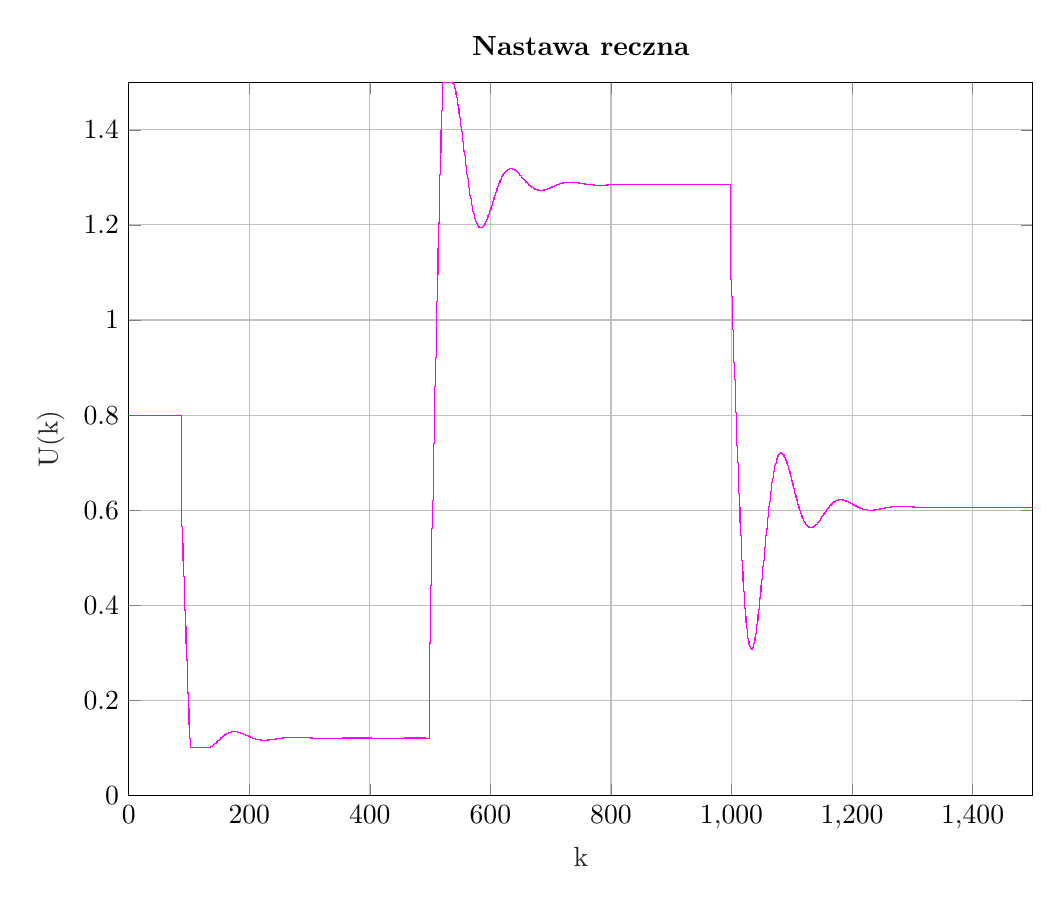
\begin{tikzpicture}

\begin{axis}[%
width=4.521in,
height=3.566in,
at={(0.758in,0.481in)},
scale only axis,
xmin=0,
xmax=1500,
xlabel style={font=\color{white!15!black}},
xlabel={k},
ymin=0,
ymax=1.5,
ylabel style={font=\color{white!15!black}},
ylabel={U(k)},
axis background/.style={fill=white},
title style={font=\bfseries},
title={Nastawa reczna},
xmajorgrids,
ymajorgrids,
legend style={legend cell align=left, align=left, draw=white!15!black}
]
\addplot[const plot, color=mycolor1] table[row sep=crcr] {%
0	0.8\\
1	0.8\\
2	0.8\\
3	0.8\\
4	0.8\\
5	0.8\\
6	0.8\\
7	0.8\\
8	0.8\\
9	0.8\\
10	0.8\\
11	0.8\\
12	0.8\\
13	0.8\\
14	0.8\\
15	0.8\\
16	0.8\\
17	0.8\\
18	0.8\\
19	0.8\\
20	0.8\\
21	0.8\\
22	0.8\\
23	0.8\\
24	0.8\\
25	0.8\\
26	0.8\\
27	0.8\\
28	0.8\\
29	0.8\\
30	0.8\\
31	0.8\\
32	0.8\\
33	0.8\\
34	0.8\\
35	0.8\\
36	0.8\\
37	0.8\\
38	0.8\\
39	0.8\\
40	0.8\\
41	0.8\\
42	0.8\\
43	0.8\\
44	0.8\\
45	0.8\\
46	0.8\\
47	0.8\\
48	0.8\\
49	0.8\\
50	0.8\\
51	0.8\\
52	0.8\\
53	0.8\\
54	0.8\\
55	0.8\\
56	0.8\\
57	0.8\\
58	0.8\\
59	0.8\\
60	0.8\\
61	0.8\\
62	0.8\\
63	0.8\\
64	0.8\\
65	0.8\\
66	0.8\\
67	0.8\\
68	0.8\\
69	0.8\\
70	0.8\\
71	0.8\\
72	0.8\\
73	0.8\\
74	0.8\\
75	0.8\\
76	0.8\\
77	0.8\\
78	0.8\\
79	0.8\\
80	0.8\\
81	0.8\\
82	0.8\\
83	0.8\\
84	0.8\\
85	0.8\\
86	0.8\\
87	0.6\\
88	0.565\\
89	0.53\\
90	0.495\\
91	0.46\\
92	0.425\\
93	0.390000000000001\\
94	0.355000000000001\\
95	0.320000000000001\\
96	0.285000000000001\\
97	0.250000000000001\\
98	0.215557005500001\\
99	0.182241417241901\\
100	0.15012991341864\\
101	0.119291206543686\\
102	0.1\\
103	0.1\\
104	0.1\\
105	0.1\\
106	0.1\\
107	0.1\\
108	0.1\\
109	0.1\\
110	0.1\\
111	0.1\\
112	0.1\\
113	0.1\\
114	0.1\\
115	0.1\\
116	0.1\\
117	0.1\\
118	0.1\\
119	0.1\\
120	0.1\\
121	0.1\\
122	0.1\\
123	0.1\\
124	0.1\\
125	0.1\\
126	0.1\\
127	0.1\\
128	0.1\\
129	0.1\\
130	0.1\\
131	0.1\\
132	0.100113821997798\\
133	0.100394589391308\\
134	0.100822300382422\\
135	0.101379079341974\\
136	0.10204896239458\\
137	0.102817704065704\\
138	0.103672602950572\\
139	0.104602344560704\\
140	0.105596859681222\\
141	0.106647196732502\\
142	0.107745406774753\\
143	0.108884122927885\\
144	0.110056049993399\\
145	0.111253869494611\\
146	0.112470341824546\\
147	0.113698387335029\\
148	0.114931149555416\\
149	0.116162043307158\\
150	0.117384790110044\\
151	0.118593442951334\\
152	0.119782402204802\\
153	0.120946424238122\\
154	0.122080624912709\\
155	0.123180481018959\\
156	0.124241831466181\\
157	0.125260878216979\\
158	0.126234186494426\\
159	0.127158683943357\\
160	0.128031658548611\\
161	0.128850755208539\\
162	0.129613970935826\\
163	0.13031964871364\\
164	0.130966470076365\\
165	0.131553446511115\\
166	0.132079909786107\\
167	0.132545501307659\\
168	0.132950160598986\\
169	0.133294112987418\\
170	0.133577856582992\\
171	0.13380214862934\\
172	0.133967991306802\\
173	0.134076617067123\\
174	0.134129473578494\\
175	0.13412820835896\\
176	0.134074653175016\\
177	0.133970808280579\\
178	0.133818826569494\\
179	0.133620997712331\\
180	0.133379732345598\\
181	0.133097546378615\\
182	0.132777045480296\\
183	0.13242090980489\\
184	0.132031879012451\\
185	0.131612737636411\\
186	0.131166300847109\\
187	0.130695400656607\\
188	0.13020287260645\\
189	0.129691542976386\\
190	0.129164216548357\\
191	0.128623664956373\\
192	0.128072615649185\\
193	0.127513741489003\\
194	0.126949651005884\\
195	0.126382879323836\\
196	0.125815879771183\\
197	0.125251016184298\\
198	0.124690555910511\\
199	0.124136663512724\\
200	0.1235913951752\\
201	0.123056693806951\\
202	0.122534384836333\\
203	0.122026172687705\\
204	0.121533637928425\\
205	0.121058235072059\\
206	0.120601291021369\\
207	0.120164004132546\\
208	0.119747443880215\\
209	0.11935255110092\\
210	0.118980138791188\\
211	0.118630893434831\\
212	0.118305376832813\\
213	0.118004028407918\\
214	0.117727167955478\\
215	0.117474998810608\\
216	0.117247611401778\\
217	0.117044987160037\\
218	0.116867002752883\\
219	0.116713434611579\\
220	0.116583963720673\\
221	0.116478180638563\\
222	0.116395590718165\\
223	0.116335619497099\\
224	0.116297618227276\\
225	0.116280869514318\\
226	0.116284593037952\\
227	0.116307951325303\\
228	0.116350055549841\\
229	0.116409971329754\\
230	0.116486724500488\\
231	0.116579306837339\\
232	0.116686681705125\\
233	0.116807789613183\\
234	0.1169415536552\\
235	0.11708688481469\\
236	0.11724268711826\\
237	0.117407862620173\\
238	0.117581316203083\\
239	0.117761960181217\\
240	0.117948718693666\\
241	0.118140531876856\\
242	0.118336359806618\\
243	0.11853518620171\\
244	0.118736021881932\\
245	0.11893790797537\\
246	0.119139918870559\\
247	0.119341164910655\\
248	0.11954079482794\\
249	0.119737997918151\\
250	0.119932005955312\\
251	0.120122094848815\\
252	0.12030758604557\\
253	0.120487847681026\\
254	0.120662295483817\\
255	0.120830393439661\\
256	0.120991654220988\\
257	0.121145639389508\\
258	0.12129195937965\\
259	0.121430273271463\\
260	0.121560288362102\\
261	0.121681759545602\\
262	0.121794488511044\\
263	0.12189832276964\\
264	0.121993154521597\\
265	0.122078919373875\\
266	0.122155594920195\\
267	0.122223199194774\\
268	0.122281789011407\\
269	0.122331458199524\\
270	0.122372335748865\\
271	0.122404583874357\\
272	0.12242839601267\\
273	0.122443994761774\\
274	0.122451629774644\\
275	0.122451575617993\\
276	0.122444129606688\\
277	0.122429609624139\\
278	0.122408351938669\\
279	0.122380709025452\\
280	0.122347047403247\\
281	0.122307745494706\\
282	0.122263191518608\\
283	0.122213781421892\\
284	0.122159916858915\\
285	0.122102003224816\\
286	0.122040447749413\\
287	0.12197565765753\\
288	0.121908038401125\\
289	0.121837991968078\\
290	0.121765915271989\\
291	0.12169219862679\\
292	0.121617224309479\\
293	0.121541365213772\\
294	0.121464983596955\\
295	0.121388429921742\\
296	0.121312041794443\\
297	0.121236143000302\\
298	0.121161042636384\\
299	0.121087034341981\\
300	0.121014395626056\\
301	0.120943387290876\\
302	0.12087425295056\\
303	0.120807218642956\\
304	0.12074249253286\\
305	0.120680264704344\\
306	0.120620707039573\\
307	0.12056397318131\\
308	0.120510198575979\\
309	0.120459500593976\\
310	0.120411978723691\\
311	0.120367714835528\\
312	0.120326773512049\\
313	0.120289202440241\\
314	0.120255032861776\\
315	0.120224280077062\\
316	0.12019694399879\\
317	0.12017300975067\\
318	0.120152448306977\\
319	0.120135217168562\\
320	0.120121261070962\\
321	0.120110512720308\\
322	0.120102893552736\\
323	0.120098314513108\\
324	0.120096676848908\\
325	0.120097872915288\\
326	0.120101786987323\\
327	0.120108296075693\\
328	0.120117270742112\\
329	0.120128575910974\\
330	0.120142071673852\\
331	0.120157614083646\\
332	0.120175055935319\\
333	0.120194247530387\\
334	0.120215037422457\\
335	0.120237273141331\\
336	0.120260801893372\\
337	0.120285471236013\\
338	0.120311129724503\\
339	0.12033762752915\\
340	0.120364817021553\\
341	0.120392553328477\\
342	0.120420694852235\\
343	0.120449103756616\\
344	0.120477646417615\\
345	0.120506193838351\\
346	0.120534622027801\\
347	0.120562812343088\\
348	0.120590651795281\\
349	0.120618033318787\\
350	0.12064485600459\\
351	0.120671025297738\\
352	0.120696453159601\\
353	0.120721058195585\\
354	0.120744765749079\\
355	0.120767507962544\\
356	0.120789223806773\\
357	0.120809859079413\\
358	0.120829366373964\\
359	0.120847705020539\\
360	0.120864840999738\\
361	0.120880746831056\\
362	0.120895401437299\\
363	0.12090878998653\\
364	0.120920903713113\\
365	0.120931739719428\\
366	0.120941300759881\\
367	0.120949595008834\\
368	0.120956635814078\\
369	0.120962441437491\\
370	0.120967034784496\\
371	0.120970443123928\\
372	0.120972697799908\\
373	0.120973833937266\\
374	0.120973890142053\\
375	0.120972908198632\\
376	0.120970932764787\\
377	0.120968011066251\\
378	0.120964192592002\\
379	0.120959528791615\\
380	0.1209540727759\\
381	0.120947879022005\\
382	0.120941003084073\\
383	0.1209335013105\\
384	0.120925430568764\\
385	0.120916847978718\\
386	0.120907810655174\\
387	0.120898375460538\\
388	0.120888598768159\\
389	0.12087853623703\\
390	0.120868242598343\\
391	0.120857771454388\\
392	0.120847175090167\\
393	0.120836504298062\\
394	0.120825808215788\\
395	0.120815134177844\\
396	0.120804527580544\\
397	0.120794031760723\\
398	0.12078368788808\\
399	0.120773534871111\\
400	0.120763609276503\\
401	0.120753945261818\\
402	0.120744574521242\\
403	0.120735526244119\\
404	0.12072682708596\\
405	0.120718501151557\\
406	0.120710569989823\\
407	0.120703052599891\\
408	0.120695965448048\\
409	0.120689322494971\\
410	0.120683135232772\\
411	0.120677412731296\\
412	0.120672161693116\\
413	0.120667386516649\\
414	0.120663089366794\\
415	0.120659270252512\\
416	0.120655927110718\\
417	0.120653055895895\\
418	0.120650650674807\\
419	0.120648703725708\\
420	0.120647205641441\\
421	0.120646145435823\\
422	0.120645510652737\\
423	0.120645287477347\\
424	0.120645460848866\\
425	0.12064601457434\\
426	0.120646931442907\\
427	0.120648193340018\\
428	0.120649781361127\\
429	0.120651675924382\\
430	0.120653856881859\\
431	0.120656303628925\\
432	0.120658995211312\\
433	0.120661910429553\\
434	0.120665027940399\\
435	0.120668326354918\\
436	0.120671784332976\\
437	0.120675380673819\\
438	0.120679094402533\\
439	0.120682904852151\\
440	0.120686791741236\\
441	0.120690735246768\\
442	0.120694716072205\\
443	0.12069871551062\\
444	0.120702715502811\\
445	0.120706698690359\\
446	0.120710648463565\\
447	0.12071454900429\\
448	0.120718385323685\\
449	0.120722143294869\\
450	0.120725809680589\\
451	0.120729372155952\\
452	0.12073281932632\\
453	0.12073614074047\\
454	0.120739326899161\\
455	0.120742369259233\\
456	0.12074526023341\\
457	0.120747993185963\\
458	0.120750562424422\\
459	0.120752963187517\\
460	0.12075519162956\\
461	0.120757244801459\\
462	0.120759120628594\\
463	0.120760817885754\\
464	0.120762336169379\\
465	0.120763675867315\\
466	0.120764838126319\\
467	0.12076582481754\\
468	0.120766638500204\\
469	0.120767282383729\\
470	0.120767760288504\\
471	0.120768076605538\\
472	0.120768236255212\\
473	0.120768244645344\\
474	0.120768107628769\\
475	0.12076783146065\\
476	0.120767422755697\\
477	0.120766888445503\\
478	0.120766235736161\\
479	0.120765472066347\\
480	0.120764605066022\\
481	0.120763642515917\\
482	0.12076259230794\\
483	0.12076146240664\\
484	0.120760260811867\\
485	0.120758995522716\\
486	0.120757674502896\\
487	0.120756305647586\\
488	0.120754896751891\\
489	0.120753455480948\\
490	0.120751989341769\\
491	0.12075050565686\\
492	0.12074901153967\\
493	0.120747513871899\\
494	0.120746019282695\\
495	0.120744534129758\\
496	0.120743064482354\\
497	0.120741616106238\\
498	0.120740194450486\\
499	0.320740194450486\\
500	0.38073884126139\\
501	0.440737529136205\\
502	0.50073626216286\\
503	0.560735044074431\\
504	0.620733878246776\\
505	0.680732767697815\\
506	0.740731715088383\\
507	0.800730722724603\\
508	0.860729792561703\\
509	0.920728926209202\\
510	0.980171115566723\\
511	1.03841633185725\\
512	1.09525915693866\\
513	1.15051508291567\\
514	1.20401844814761\\
515	1.2556205737261\\
516	1.30518808112149\\
517	1.35260137354628\\
518	1.39775326525637\\
519	1.4405477445237\\
520	1.4808988573819\\
521	1.5\\
522	1.5\\
523	1.5\\
524	1.5\\
525	1.5\\
526	1.5\\
527	1.5\\
528	1.5\\
529	1.5\\
530	1.5\\
531	1.5\\
532	1.5\\
533	1.5\\
534	1.5\\
535	1.5\\
536	1.5\\
537	1.49967566598337\\
538	1.49805067082329\\
539	1.49526384873921\\
540	1.49144000528331\\
541	1.48669129680977\\
542	1.4811184762346\\
543	1.47481201794491\\
544	1.46785313348546\\
545	1.46031468853639\\
546	1.45226203068887\\
547	1.44375373661439\\
548	1.43484318967851\\
549	1.42558267449311\\
550	1.41602568003694\\
551	1.40622606212796\\
552	1.39623736212486\\
553	1.38611225926437\\
554	1.3759021369512\\
555	1.36565674587817\\
556	1.35542394910316\\
557	1.34524953618516\\
558	1.33517709521414\\
559	1.32524793057251\\
560	1.31550100626667\\
561	1.30597289501387\\
562	1.29669772873761\\
563	1.28770715442993\\
564	1.27903029815657\\
565	1.27069373903072\\
566	1.26272149422535\\
567	1.2551350155007\\
568	1.24795319726468\\
569	1.24119239583642\\
570	1.23486645933386\\
571	1.22898676747095\\
572	1.22356228053638\\
573	1.21859959687866\\
574	1.21410301827056\\
575	1.21007462255121\\
576	1.20651434295471\\
577	1.20342005353611\\
578	1.20078766010293\\
579	1.19861119605775\\
580	1.19688292255481\\
581	1.19559343237508\\
582	1.19473175692837\\
583	1.19428547579922\\
584	1.19424082826465\\
585	1.19458282622519\\
586	1.19529536800696\\
587	1.19636135250937\\
588	1.19776279319278\\
589	1.19948093142032\\
590	1.20149634869002\\
591	1.20378907731622\\
592	1.20633870914274\\
593	1.20912450189526\\
594	1.21212548280564\\
595	1.21532054916692\\
596	1.21868856550422\\
597	1.22220845707377\\
598	1.22585929942915\\
599	1.22962040382105\\
600	1.23347139822398\\
601	1.23739230381023\\
602	1.24136360671816\\
603	1.24536632498794\\
604	1.24938207056411\\
605	1.25339310628914\\
606	1.2573823978371\\
607	1.26133366056022\\
608	1.26523140124433\\
609	1.26906095479122\\
610	1.27280851586729\\
611	1.27646116557811\\
612	1.28000689324762\\
613	1.28343461339895\\
614	1.28673417805063\\
615	1.28989638445816\\
616	1.29291297844505\\
617	1.29577665348141\\
618	1.2984810456801\\
619	1.30102072489159\\
620	1.30339118208865\\
621	1.30558881324026\\
622	1.30761089988203\\
623	1.30945558659615\\
624	1.31112185561944\\
625	1.31260949880154\\
626	1.31391908713852\\
627	1.31505193810858\\
628	1.31601008103736\\
629	1.31679622072007\\
630	1.31741369952616\\
631	1.31786645821026\\
632	1.31815899564987\\
633	1.31829632772625\\
634	1.3182839455605\\
635	1.31812777331109\\
636	1.317834125733\\
637	1.31740966569205\\
638	1.31686136182042\\
639	1.3161964464916\\
640	1.31542237428465\\
641	1.31454678109897\\
642	1.31357744407157\\
643	1.31252224243948\\
644	1.31138911948036\\
645	1.31018604565427\\
646	1.30892098305996\\
647	1.30760185130839\\
648	1.30623649490666\\
649	1.30483265223468\\
650	1.30339792618745\\
651	1.30193975654525\\
652	1.30046539412442\\
653	1.29898187675144\\
654	1.29749600709368\\
655	1.29601433237056\\
656	1.29454312596007\\
657	1.2930883709065\\
658	1.29165574532706\\
659	1.2902506097067\\
660	1.28887799606274\\
661	1.28754259895358\\
662	1.28624876829878\\
663	1.28500050397092\\
664	1.28380145211414\\
665	1.28265490313778\\
666	1.28156379132885\\
667	1.280530696022\\
668	1.2795578442613\\
669	1.27864711488424\\
670	1.27780004395499\\
671	1.2770178314708\\
672	1.27630134926301\\
673	1.27565115001191\\
674	1.27506747729308\\
675	1.27455027657146\\
676	1.27409920705882\\
677	1.27371365434945\\
678	1.27339274374909\\
679	1.27313535421253\\
680	1.27294013280552\\
681	1.2728055096082\\
682	1.2727297129781\\
683	1.27271078509266\\
684	1.27274659769311\\
685	1.27283486795344\\
686	1.27297317440115\\
687	1.27315897281851\\
688	1.27338961205631\\
689	1.273662349695\\
690	1.27397436749123\\
691	1.27432278655133\\
692	1.27470468217647\\
693	1.27511709832808\\
694	1.2755570616656\\
695	1.27602159511231\\
696	1.27650773090899\\
697	1.27701252311862\\
698	1.27753305954941\\
699	1.27806647306714\\
700	1.27860995227154\\
701	1.27916075151518\\
702	1.27971620024714\\
703	1.28027371166723\\
704	1.28083079068004\\
705	1.28138504114175\\
706	1.28193417239563\\
707	1.28247600509591\\
708	1.28300847632216\\
709	1.28352964398989\\
710	1.28403769056558\\
711	1.28453092609707\\
712	1.28500779057294\\
713	1.28546685562674\\
714	1.28590682560417\\
715	1.28632653801346\\
716	1.28672496338092\\
717	1.28710120453559\\
718	1.28745449534817\\
719	1.2877841989511\\
720	1.28808980546755\\
721	1.28837092927841\\
722	1.28862730585709\\
723	1.28885878820264\\
724	1.28906534290234\\
725	1.28924704585521\\
726	1.28940407768819\\
727	1.28953671889692\\
728	1.28964534474271\\
729	1.28973041993748\\
730	1.28979249314796\\
731	1.28983219134985\\
732	1.28985021406247\\
733	1.28984732749333\\
734	1.28982435862174\\
735	1.28978218924919\\
736	1.28972175004391\\
737	1.28964401460532\\
738	1.28954999357364\\
739	1.28944072880812\\
740	1.28931728765674\\
741	1.28918075733843\\
742	1.28903223945793\\
743	1.28887284467181\\
744	1.28870368752289\\
745	1.288525881459\\
746	1.28834053405031\\
747	1.28814874241842\\
748	1.28795158888858\\
749	1.2877501368754\\
750	1.28754542701064\\
751	1.2873384735205\\
752	1.28713026085836\\
753	1.28692174059774\\
754	1.28671382858858\\
755	1.28650740237916\\
756	1.28630329890438\\
757	1.28610231243997\\
758	1.28590519282134\\
759	1.2857126439243\\
760	1.28552532240412\\
761	1.28534383668836\\
762	1.2851687462179\\
763	1.28500056092986\\
764	1.28483974097509\\
765	1.28468669666259\\
766	1.28454178862195\\
767	1.28440532817486\\
768	1.28427757790581\\
769	1.28415875242182\\
770	1.28404901929048\\
771	1.28394850014538\\
772	1.2838572719475\\
773	1.28377536839122\\
774	1.28370278144293\\
775	1.28363946300074\\
776	1.28358532666311\\
777	1.28354024959465\\
778	1.2835040744772\\
779	1.2834766115343\\
780	1.28345764061763\\
781	1.28344691334374\\
782	1.28344415527\\
783	1.28344906809877\\
784	1.28346133189909\\
785	1.28348060733571\\
786	1.28350653789532\\
787	1.28353875210063\\
788	1.28357686570306\\
789	1.28362048384542\\
790	1.28366920318632\\
791	1.28372261397873\\
792	1.28378030209521\\
793	1.28384185099347\\
794	1.28390684361568\\
795	1.28397486421615\\
796	1.28404550011219\\
797	1.28411834335344\\
798	1.28419299230574\\
799	1.28426905314597\\
800	1.28434614126477\\
801	1.28442388257477\\
802	1.28450191472229\\
803	1.2845798882009\\
804	1.28465746736607\\
805	1.28473433135018\\
806	1.28481017487782\\
807	1.28488470898183\\
808	1.28495766162076\\
809	1.28502877819891\\
810	1.28509782199051\\
811	1.28516457446998\\
812	1.28522883555042\\
813	1.28529042373283\\
814	1.28534917616912\\
815	1.28540494864168\\
816	1.28545761546305\\
817	1.28550706929922\\
818	1.28555322092022\\
819	1.28559599888198\\
820	1.28563534914346\\
821	1.28567123462333\\
822	1.2857036347003\\
823	1.28573254466167\\
824	1.28575797510435\\
825	1.28577995129283\\
826	1.28579851247864\\
827	1.28581371118561\\
828	1.28582561246552\\
829	1.28583429312835\\
830	1.28583984095158\\
831	1.28584235387278\\
832	1.28584193916951\\
833	1.28583871263076\\
834	1.28583279772372\\
835	1.2858243247597\\
836	1.2858134300629\\
837	1.28580025514545\\
838	1.28578494589213\\
839	1.28576765175779\\
840	1.2857485249807\\
841	1.28572771981427\\
842	1.28570539178013\\
843	1.28568169694468\\
844	1.28565679122151\\
845	1.28563082970157\\
846	1.28560396601307\\
847	1.28557635171262\\
848	1.28554813570897\\
849	1.28551946372081\\
850	1.28549047776936\\
851	1.28546131570687\\
852	1.28543211078142\\
853	1.28540299123875\\
854	1.28537407996117\\
855	1.2853454941438\\
856	1.28531734500811\\
857	1.28528973755246\\
858	1.28526277033933\\
859	1.28523653531871\\
860	1.28521111768709\\
861	1.28518659578112\\
862	1.28516304100525\\
863	1.2851405177921\\
864	1.2851190835947\\
865	1.28509878890924\\
866	1.28507967732708\\
867	1.28506178561464\\
868	1.28504514381986\\
869	1.28502977540347\\
870	1.28501569739386\\
871	1.28500292056368\\
872	1.28499144962674\\
873	1.28498128345348\\
874	1.28497241530341\\
875	1.28496483307274\\
876	1.28495851955569\\
877	1.28495345271771\\
878	1.28494960597899\\
879	1.28494694850663\\
880	1.28494544551386\\
881	1.28494505856476\\
882	1.28494574588294\\
883	1.28494746266264\\
884	1.28495016138088\\
885	1.28495379210925\\
886	1.2849583028239\\
887	1.28496363971267\\
888	1.28496974747791\\
889	1.28497656963395\\
890	1.28498404879825\\
891	1.28499212697493\\
892	1.28500074583009\\
893	1.28500984695771\\
894	1.28501937213568\\
895	1.28502926357091\\
896	1.28503946413312\\
897	1.28504991757668\\
898	1.28506056874988\\
899	1.2850713637914\\
900	1.2850822503135\\
901	1.2850931775717\\
902	1.28510409662072\\
903	1.28511496045657\\
904	1.28512572414468\\
905	1.28513634493405\\
906	1.28514678235756\\
907	1.28515699831841\\
908	1.28516695716294\\
909	1.28517662574004\\
910	1.28518597344737\\
911	1.28519497226479\\
912	1.28520359677524\\
913	1.28521182417355\\
914	1.28521963426357\\
915	1.28522700944414\\
916	1.28523393468433\\
917	1.2852403974885\\
918	1.28524638785177\\
919	1.28525189820637\\
920	1.28525692335957\\
921	1.28526146042372\\
922	1.28526550873898\\
923	1.28526906978948\\
924	1.2852721471134\\
925	1.28527474620762\\
926	1.28527687442771\\
927	1.28527854088361\\
928	1.28527975633187\\
929	1.28528053306493\\
930	1.28528088479803\\
931	1.28528082655435\\
932	1.28528037454901\\
933	1.28527954607237\\
934	1.28527835937323\\
935	1.2852768335424\\
936	1.2852749883972\\
937	1.28527284436729\\
938	1.28527042238225\\
939	1.28526774376144\\
940	1.2852648301064\\
941	1.28526170319628\\
942	1.28525838488647\\
943	1.28525489701096\\
944	1.28525126128854\\
945	1.28524749923312\\
946	1.28524363206851\\
947	1.28523968064769\\
948	1.28523566537689\\
949	1.28523160614456\\
950	1.2852275222553\\
951	1.28522343236892\\
952	1.28521935444474\\
953	1.28521530569093\\
954	1.28521130251925\\
955	1.28520736050491\\
956	1.28520349435161\\
957	1.28519971786178\\
958	1.28519604391184\\
959	1.28519248443244\\
960	1.28518905039358\\
961	1.28518575179449\\
962	1.28518259765806\\
963	1.28517959602974\\
964	1.28517675398078\\
965	1.28517407761546\\
966	1.28517157208232\\
967	1.28516924158903\\
968	1.28516708942081\\
969	1.28516511796209\\
970	1.28516332872126\\
971	1.28516172235824\\
972	1.28516029871466\\
973	1.28515905684637\\
974	1.2851579950582\\
975	1.28515711094047\\
976	1.28515640140731\\
977	1.28515586273634\\
978	1.28515549060958\\
979	1.28515528015535\\
980	1.28515522599099\\
981	1.28515532226601\\
982	1.28515556270571\\
983	1.28515594065491\\
984	1.28515644912153\\
985	1.28515708082011\\
986	1.28515782821471\\
987	1.28515868356143\\
988	1.28515963894996\\
989	1.28516068634443\\
990	1.28516181762307\\
991	1.28516302461679\\
992	1.28516429914642\\
993	1.28516563305852\\
994	1.28516701825978\\
995	1.28516844674968\\
996	1.28516991065161\\
997	1.28517140224216\\
998	1.28517291397864\\
999	1.08517291397864\\
1000	1.05017444422806\\
1001	1.01517597332662\\
1002	0.98017749469193\\
1003	0.945179002031408\\
1004	0.910180489358272\\
1005	0.875181951005574\\
1006	0.840183381638304\\
1007	0.805184776263596\\
1008	0.770186130239041\\
1009	0.735187439279161\\
1010	0.700745709205993\\
1011	0.667431340807084\\
1012	0.635321008292402\\
1013	0.604483420635243\\
1014	0.574980115916229\\
1015	0.546866178092588\\
1016	0.520190883683773\\
1017	0.494998285145552\\
1018	0.471327737054536\\
1019	0.449214370637152\\
1020	0.428689521645345\\
1021	0.409779564813014\\
1022	0.392503355844427\\
1023	0.376871270839468\\
1024	0.362885671434006\\
1025	0.350541365935388\\
1026	0.339826062564707\\
1027	0.330720811718676\\
1028	0.323200434846483\\
1029	0.317233938116189\\
1030	0.312784909534782\\
1031	0.309811898597644\\
1032	0.308268782207891\\
1033	0.308105128332472\\
1034	0.309266566952634\\
1035	0.311695168717752\\
1036	0.315329827914835\\
1037	0.320106646741799\\
1038	0.325959318230199\\
1039	0.332819505500177\\
1040	0.340617215345525\\
1041	0.349281164439096\\
1042	0.358739136718138\\
1043	0.368918330743609\\
1044	0.379745695996719\\
1045	0.391148257171215\\
1046	0.403053425579228\\
1047	0.415389296850143\\
1048	0.428084934174676\\
1049	0.441070636427115\\
1050	0.454278190584672\\
1051	0.467641107951893\\
1052	0.481094843788082\\
1053	0.49457700002504\\
1054	0.508027510849858\\
1055	0.521388811012052\\
1056	0.534605986795591\\
1057	0.547626909674222\\
1058	0.560402352742985\\
1059	0.572886090089824\\
1060	0.585034979338767\\
1061	0.596809027660011\\
1062	0.608171441602485\\
1063	0.619088661160746\\
1064	0.629530378540453\\
1065	0.639469542135017\\
1066	0.648882346270221\\
1067	0.657748207313737\\
1068	0.666049726782392\\
1069	0.673772642111807\\
1070	0.680905765780733\\
1071	0.687440913505971\\
1072	0.693372822243327\\
1073	0.698699058745643\\
1074	0.703419919440733\\
1075	0.707538322399957\\
1076	0.711059692172557\\
1077	0.713991838261626\\
1078	0.716344828014996\\
1079	0.718130854698465\\
1080	0.71936410150984\\
1081	0.720060602280363\\
1082	0.720238099595419\\
1083	0.719915901049155\\
1084	0.719114734327938\\
1085	0.71785660179562\\
1086	0.716164635229591\\
1087	0.714062951330692\\
1088	0.711576508602474\\
1089	0.70873096616622\\
1090	0.705552545047694\\
1091	0.702067892440071\\
1092	0.698303949414938\\
1093	0.694287822520005\\
1094	0.690046659668236\\
1095	0.685607530688783\\
1096	0.680997312875503\\
1097	0.676242581834118\\
1098	0.671369507894422\\
1099	0.666403758319447\\
1100	0.661370405509368\\
1101	0.656293841364284\\
1102	0.6511976979369\\
1103	0.646104774473828\\
1104	0.641036970912683\\
1105	0.636015227871576\\
1106	0.631059473138053\\
1107	0.626188574636097\\
1108	0.621420299822582\\
1109	0.6167712814386\\
1110	0.612256989516459\\
1111	0.607891709519902\\
1112	0.603688526473303\\
1113	0.599659314915262\\
1114	0.595814734493178\\
1115	0.592164230998113\\
1116	0.588716042623468\\
1117	0.585477211216811\\
1118	0.582453598281539\\
1119	0.579649905473941\\
1120	0.577069699331676\\
1121	0.574715439961608\\
1122	0.572588513408386\\
1123	0.570689267420065\\
1124	0.569017050323378\\
1125	0.567570252718993\\
1126	0.56634635170616\\
1127	0.565341957346489\\
1128	0.564552861078222\\
1129	0.563974085795129\\
1130	0.563599937308111\\
1131	0.563424056912532\\
1132	0.563439474790351\\
1133	0.56363866398302\\
1134	0.564013594678939\\
1135	0.564555788567873\\
1136	0.565256373024094\\
1137	0.566106134890019\\
1138	0.567095573642747\\
1139	0.568214953737045\\
1140	0.569454355929938\\
1141	0.570803727404067\\
1142	0.572252930519303\\
1143	0.573791790034687\\
1144	0.575410138655559\\
1145	0.577097860773639\\
1146	0.578844934280803\\
1147	0.580641470350313\\
1148	0.582477751092177\\
1149	0.58434426500218\\
1150	0.586231740136835\\
1151	0.588131174958964\\
1152	0.590033866810913\\
1153	0.591931437984316\\
1154	0.593815859367001\\
1155	0.595679471658831\\
1156	0.597515004159195\\
1157	0.599315591139218\\
1158	0.601074785821777\\
1159	0.60278657200184\\
1160	0.604445373348623\\
1161	0.606046060439495\\
1162	0.607583955583441\\
1163	0.609054835499227\\
1164	0.610454931920169\\
1165	0.611780930203605\\
1166	0.613029966028765\\
1167	0.614199620271769\\
1168	0.615287912150925\\
1169	0.616293290739374\\
1170	0.617214624945411\\
1171	0.618051192063581\\
1172	0.618802665001781\\
1173	0.619469098291288\\
1174	0.620050912987708\\
1175	0.620548880571472\\
1176	0.620964105956591\\
1177	0.62129800971603\\
1178	0.62155230963122\\
1179	0.62172900167199\\
1180	0.621830340511524\\
1181	0.621858819678881\\
1182	0.621817151449205\\
1183	0.621708246568998\\
1184	0.621535193910731\\
1185	0.621301240147723\\
1186	0.621009769536584\\
1187	0.620664283890653\\
1188	0.62026838282378\\
1189	0.619825744339554\\
1190	0.619340105836643\\
1191	0.618815245596367\\
1192	0.61825496481396\\
1193	0.617663070230217\\
1194	0.617043357415437\\
1195	0.61639959475269\\
1196	0.61573550816261\\
1197	0.615054766607032\\
1198	0.614360968403979\\
1199	0.613657628381713\\
1200	0.612948165894861\\
1201	0.612235893720971\\
1202	0.61152400785136\\
1203	0.610815578185655\\
1204	0.610113540135194\\
1205	0.609420687136267\\
1206	0.608739664070229\\
1207	0.608072961583697\\
1208	0.607422911298382\\
1209	0.606791681896693\\
1210	0.606181276065977\\
1211	0.605593528281191\\
1212	0.605030103402988\\
1213	0.604492496065531\\
1214	0.603982030825943\\
1215	0.60349986304509\\
1216	0.603046980467396\\
1217	0.602624205465639\\
1218	0.602232197915089\\
1219	0.601871458660045\\
1220	0.601542333534658\\
1221	0.601245017899058\\
1222	0.600979561651036\\
1223	0.600745874673056\\
1224	0.600543732674038\\
1225	0.600372783385222\\
1226	0.600232553069467\\
1227	0.600122453303569\\
1228	0.600041787993591\\
1229	0.599989760583693\\
1230	0.599965481419717\\
1231	0.599967975229568\\
1232	0.599996188683422\\
1233	0.600048997997902\\
1234	0.600125216549532\\
1235	0.600223602464125\\
1236	0.600342866150144\\
1237	0.600481677745561\\
1238	0.600638674449322\\
1239	0.600812467710112\\
1240	0.60100165024685\\
1241	0.601204802877006\\
1242	0.60142050113065\\
1243	0.601647321629902\\
1244	0.601883848215267\\
1245	0.60212867780216\\
1246	0.602380425952746\\
1247	0.602637732150023\\
1248	0.602899264762889\\
1249	0.603163725692703\\
1250	0.603429854693608\\
1251	0.603696433360582\\
1252	0.603962288780881\\
1253	0.604226296846148\\
1254	0.604487385224048\\
1255	0.604744535989802\\
1256	0.604996787919466\\
1257	0.605243238448168\\
1258	0.605483045297885\\
1259	0.605715427780549\\
1260	0.60593966778349\\
1261	0.606155110445305\\
1262	0.606361164531284\\
1263	0.606557302518455\\
1264	0.606743060401198\\
1265	0.606918037229131\\
1266	0.607081894389718\\
1267	0.607234354648631\\
1268	0.607375200961456\\
1269	0.607504275070814\\
1270	0.607621475903311\\
1271	0.607726757781065\\
1272	0.607820128462792\\
1273	0.607901647029563\\
1274	0.607971421630443\\
1275	0.608029607103252\\
1276	0.60807640248561\\
1277	0.608112048431323\\
1278	0.608136824547005\\
1279	0.608151046663572\\
1280	0.608155064056981\\
1281	0.608149256632221\\
1282	0.608134032084211\\
1283	0.608109823048789\\
1284	0.608077084256538\\
1285	0.608036289701671\\
1286	0.607987929837655\\
1287	0.607932508810698\\
1288	0.607870541741596\\
1289	0.607802552065861\\
1290	0.607729068941366\\
1291	0.607650624732135\\
1292	0.607567752576197\\
1293	0.607480984044794\\
1294	0.607390846899509\\
1295	0.607297862953246\\
1296	0.607202546040261\\
1297	0.607105400099826\\
1298	0.607006917377384\\
1299	0.606907576746426\\
1300	0.606807842153663\\
1301	0.606708161189432\\
1302	0.60660896378465\\
1303	0.60651066103504\\
1304	0.606413644152774\\
1305	0.606318283545108\\
1306	0.606224928019059\\
1307	0.606133904110668\\
1308	0.606045515536901\\
1309	0.605960042767793\\
1310	0.605877742715998\\
1311	0.605798848540532\\
1312	0.605723569561104\\
1313	0.605652091279104\\
1314	0.605584575501008\\
1315	0.605521160559662\\
1316	0.605461961628701\\
1317	0.605407071125089\\
1318	0.605356559194619\\
1319	0.605310474275033\\
1320	0.605268843731302\\
1321	0.605231674557499\\
1322	0.605198954139636\\
1323	0.605170651073779\\
1324	0.605146716033752\\
1325	0.605127082682724\\
1326	0.605111668623032\\
1327	0.605100376378634\\
1328	0.605093094404658\\
1329	0.605089698118614\\
1330	0.605090050947968\\
1331	0.605094005388892\\
1332	0.605101404071165\\
1333	0.605112080824374\\
1334	0.605125861740749\\
1335	0.605142566230137\\
1336	0.605162008062874\\
1337	0.605183996396491\\
1338	0.605208336782433\\
1339	0.605234832149212\\
1340	0.605263283758651\\
1341	0.605293492132119\\
1342	0.605325257943905\\
1343	0.605358382879158\\
1344	0.605392670454028\\
1345	0.60542792679595\\
1346	0.605463961382222\\
1347	0.605500587735311\\
1348	0.605537624073557\\
1349	0.605574893916185\\
1350	0.605612226641786\\
1351	0.605649457999667\\
1352	0.605686430573668\\
1353	0.605722994198309\\
1354	0.605759006327303\\
1355	0.605794332354702\\
1356	0.605828845889125\\
1357	0.605862428981703\\
1358	0.605894972308565\\
1359	0.605926375308832\\
1360	0.60595654627926\\
1361	0.605985402426812\\
1362	0.60601286988056\\
1363	0.606038883664463\\
1364	0.606063387632644\\
1365	0.606086334368922\\
1366	0.606107685052424\\
1367	0.606127409291172\\
1368	0.606145484925619\\
1369	0.606161897804154\\
1370	0.606176641532645\\
1371	0.606189717200109\\
1372	0.606201133082629\\
1373	0.606210904327657\\
1374	0.606219052620819\\
1375	0.606225605837365\\
1376	0.606230597680355\\
1377	0.606234067307685\\
1378	0.606236058949981\\
1379	0.606236621521397\\
1380	0.606235808225261\\
1381	0.606233676156484\\
1382	0.606230285902594\\
1383	0.606225701145152\\
1384	0.606219988263289\\
1385	0.606213215940984\\
1386	0.606205454779641\\
1387	0.606196776917444\\
1388	0.606187255656873\\
1389	0.606176965101672\\
1390	0.60616597980448\\
1391	0.606154374426244\\
1392	0.606142223408411\\
1393	0.606129600658845\\
1394	0.606116579252281\\
1395	0.606103231146052\\
1396	0.606089626911731\\
1397	0.606075835483223\\
1398	0.606061923921766\\
1399	0.606047957198199\\
1400	0.606033997992764\\
1401	0.606020106512633\\
1402	0.606006340327255\\
1403	0.60599275422155\\
1404	0.605979400066886\\
1405	0.605966326709705\\
1406	0.605953579877598\\
1407	0.605941202102551\\
1408	0.605929232661035\\
1409	0.605917707530533\\
1410	0.605906659362059\\
1411	0.605896117468165\\
1412	0.605886107825886\\
1413	0.60587665309402\\
1414	0.605867772644123\\
1415	0.605859482604544\\
1416	0.605851795916795\\
1417	0.605844722403549\\
1418	0.605838268847497\\
1419	0.605832439080315\\
1420	0.60582723408096\\
1421	0.605822652082496\\
1422	0.605818688686665\\
1423	0.605815336985404\\
1424	0.605812587688501\\
1425	0.605810429256613\\
1426	0.605808848038849\\
1427	0.605807828414146\\
1428	0.605807352935681\\
1429	0.605807402477577\\
1430	0.605807956383165\\
1431	0.605808992614119\\
1432	0.605810487899761\\
1433	0.605812417885903\\
1434	0.605814757282588\\
1435	0.605817480010128\\
1436	0.605820559342887\\
1437	0.605823968050259\\
1438	0.605827678534351\\
1439	0.605831662963891\\
1440	0.60583589340394\\
1441	0.605840341940998\\
1442	0.605844980803148\\
1443	0.605849782474908\\
1444	0.605854719806501\\
1445	0.605859766117285\\
1446	0.605864895293119\\
1447	0.605870081877491\\
1448	0.60587530115624\\
1449	0.605880529235763\\
1450	0.605885743114627\\
1451	0.605890920748514\\
1452	0.605896041108505\\
1453	0.60590108423268\\
1454	0.605906031271089\\
1455	0.605910864524159\\
1456	0.605915567474608\\
1457	0.605920124813002\\
1458	0.605924522457079\\
1459	0.605928747565001\\
1460	0.605932788542713\\
1461	0.605936635045612\\
1462	0.605940277974731\\
1463	0.605943709467676\\
1464	0.605946922884555\\
1465	0.605949912789155\\
1466	0.605952674925641\\
1467	0.605955206191038\\
1468	0.605957504603797\\
1469	0.605959569268714\\
1470	0.605961400338519\\
1471	0.605962998972407\\
1472	0.605964367291827\\
1473	0.605965508333827\\
1474	0.605966426002234\\
1475	0.605967125016995\\
1476	0.605967610861935\\
1477	0.605967889731254\\
1478	0.605967968475024\\
1479	0.605967854543956\\
1480	0.605967555933729\\
1481	0.605967081129114\\
1482	0.605966439048159\\
1483	0.605965638986669\\
1484	0.605964690563205\\
1485	0.605963603664836\\
1486	0.605962388393828\\
1487	0.605961055015484\\
1488	0.605959613907306\\
1489	0.60595807550965\\
1490	0.605956450278026\\
1491	0.6059547486372\\
1492	0.605952980937203\\
1493	0.605951157411388\\
1494	0.605949288136617\\
1495	0.605947382995685\\
1496	0.605945451642038\\
1497	0.60594350346687\\
1498	0.605941547568627\\
1499	0.605939592724977\\
};


\end{axis}
\end{tikzpicture}%
\label{pidru}
\end{figure}

\begin{figure}

\centering
\caption{Przebieg symulacji PID dla parametrów dobranych metodą eksperymentalną - wartość wyjścia}
% This file was created by matlab2tikz.
%
\begin{tikzpicture}

\begin{axis}[%
width=4.521in,
height=3.566in,
at={(0.758in,0.481in)},
scale only axis,
xmin=0,
xmax=1500,
xlabel style={font=\color{white!15!black}},
xlabel={k},
ymin=1.2,
ymax=2.6,
ylabel style={font=\color{white!15!black}},
ylabel={Y(k)},
axis background/.style={fill=white},
title style={font=\bfseries},
title={Nastawa r�czna [K=1, Ti=10, Td=0]: E=76.3211},
xmajorgrids,
ymajorgrids,
legend style={legend cell align=left, align=left, draw=white!15!black}
]
\addplot[const plot, color=red] table[row sep=crcr] {%
0	2\\
1	2\\
2	2\\
3	2\\
4	2\\
5	2\\
6	2\\
7	2\\
8	2\\
9	2\\
10	2\\
11	2\\
12	2\\
13	2\\
14	2\\
15	2\\
16	2\\
17	2\\
18	2\\
19	2\\
20	2\\
21	2\\
22	2\\
23	2\\
24	2\\
25	2\\
26	2\\
27	2\\
28	2\\
29	2\\
30	2\\
31	2\\
32	2\\
33	2\\
34	2\\
35	2\\
36	2\\
37	2\\
38	2\\
39	2\\
40	2\\
41	2\\
42	2\\
43	2\\
44	2\\
45	2\\
46	2\\
47	2\\
48	2\\
49	2\\
50	2\\
51	2\\
52	2\\
53	2\\
54	2\\
55	2\\
56	2\\
57	2\\
58	2\\
59	2\\
60	2\\
61	2\\
62	2\\
63	2\\
64	2\\
65	2\\
66	2\\
67	2\\
68	2\\
69	2\\
70	2\\
71	2\\
72	2\\
73	2\\
74	2\\
75	2\\
76	2\\
77	2\\
78	2\\
79	2\\
80	2\\
81	2\\
82	2\\
83	2\\
84	2\\
85	2\\
86	2\\
87	2\\
88	2\\
89	2\\
90	2\\
91	2\\
92	2\\
93	2\\
94	2\\
95	2\\
96	2\\
97	1.99945658\\
98	1.997839759764\\
99	1.99512709228601\\
100	1.99130499693055\\
101	1.98636755194778\\
102	1.98031542157221\\
103	1.97315490383166\\
104	1.96489708657112\\
105	1.95555710044017\\
106	1.94515345871497\\
107	1.93370747483891\\
108	1.92124426291901\\
109	1.90779504791446\\
110	1.89339780467314\\
111	1.87809647486508\\
112	1.861967976203\\
113	1.8451646036605\\
114	1.82786994890366\\
115	1.81024368057372\\
116	1.79242416994124\\
117	1.77453084777699\\
118	1.75666631904614\\
119	1.73891825944436\\
120	1.72136111545526\\
121	1.7040576274958\\
122	1.68706019380645\\
123	1.67041209101822\\
124	1.65414856576983\\
125	1.63829781034067\\
126	1.62288183399348\\
127	1.60791724057214\\
128	1.59341592186253\\
129	1.57938567528786\\
130	1.56583075366376\\
131	1.55275235397499\\
132	1.54014905144596\\
133	1.52801718455483\\
134	1.51635119607942\\
135	1.50514393475593\\
136	1.49438692167406\\
137	1.48407058511935\\
138	1.47418446720121\\
139	1.46471740526893\\
140	1.45565769081554\\
141	1.44699320829552\\
142	1.43871186530243\\
143	1.43080208937011\\
144	1.42325289525331\\
145	1.41605375662638\\
146	1.4091945045856\\
147	1.40266524853714\\
148	1.39645631567997\\
149	1.39055820583911\\
150	1.38496155887985\\
151	1.37965713234574\\
152	1.37463578732076\\
153	1.36988847996405\\
154	1.3654062554719\\
155	1.36118024257354\\
156	1.35720164854479\\
157	1.35346175517436\\
158	1.34995191594739\\
159	1.34666355457897\\
160	1.34358816493129\\
161	1.34071731227387\\
162	1.33804263579435\\
163	1.33555585223099\\
164	1.33324876047851\\
165	1.33111324701615\\
166	1.32914129201872\\
167	1.32732497602627\\
168	1.32565648706067\\
169	1.32412812808642\\
170	1.32273232471991\\
171	1.32146163309702\\
172	1.32030874781393\\
173	1.31926650986069\\
174	1.31832791447191\\
175	1.31748611882347\\
176	1.31673444950958\\
177	1.31606640973944\\
178	1.31547568619816\\
179	1.3149561555219\\
180	1.31450189034227\\
181	1.31410716486052\\
182	1.3137664599165\\
183	1.31347446752296\\
184	1.31322609483993\\
185	1.313016467569\\
186	1.31284093275149\\
187	1.31269506095889\\
188	1.31257464786828\\
189	1.31247571521912\\
190	1.31239451115183\\
191	1.31232750993192\\
192	1.31227141106713\\
193	1.31222313782787\\
194	1.31217983518461\\
195	1.31213886717819\\
196	1.31209781374207\\
197	1.31205446699737\\
198	1.31200682704412\\
199	1.3119530972737\\
200	1.31189167922937\\
201	1.31182116704318\\
202	1.31174034147876\\
203	1.3116481636108\\
204	1.31154376817258\\
205	1.31142645660386\\
206	1.31129568983179\\
207	1.31115108081788\\
208	1.31099238690412\\
209	1.31081950199147\\
210	1.31063244858345\\
211	1.31043136972769\\
212	1.31021652088721\\
213	1.30998826177314\\
214	1.30974704816945\\
215	1.30949342377955\\
216	1.30922801212371\\
217	1.3089515085149\\
218	1.30866467213984\\
219	1.30836831827048\\
220	1.30806331063008\\
221	1.30775055393632\\
222	1.3074309866429\\
223	1.30710557389917\\
224	1.306775300746\\
225	1.3064411655646\\
226	1.30610417379331\\
227	1.30576533192579\\
228	1.30542564180267\\
229	1.3050860952067\\
230	1.30474766877042\\
231	1.30441131920329\\
232	1.30407797884405\\
233	1.30374855154237\\
234	1.30342390887251\\
235	1.30310488668012\\
236	1.30279228196215\\
237	1.30248685007823\\
238	1.30218930229087\\
239	1.30190030363039\\
240	1.30162047107946\\
241	1.30135037207093\\
242	1.30109052329177\\
243	1.30084138978464\\
244	1.30060338433813\\
245	1.3003768671556\\
246	1.30016214579182\\
247	1.29995947534609\\
248	1.29976905889973\\
249	1.29959104818544\\
250	1.29942554447542\\
251	1.2992725996749\\
252	1.29913221760739\\
253	1.29900435547748\\
254	1.29888892549727\\
255	1.29878579666196\\
256	1.29869479666038\\
257	1.29861571390608\\
258	1.29854829967474\\
259	1.29849227033389\\
260	1.29844730965077\\
261	1.29841307116494\\
262	1.29838918061192\\
263	1.29837523838504\\
264	1.29837082202257\\
265	1.29837548870799\\
266	1.29838877777142\\
267	1.29841021318098\\
268	1.29843930601301\\
269	1.29847555689107\\
270	1.29851845838371\\
271	1.298567497352\\
272	1.29862215723814\\
273	1.29868192028714\\
274	1.29874626969426\\
275	1.29881469167142\\
276	1.29888667742652\\
277	1.29896172505008\\
278	1.29903934130443\\
279	1.29911904331124\\
280	1.29920036013366\\
281	1.29928283425016\\
282	1.29936602291768\\
283	1.29944949942216\\
284	1.29953285421533\\
285	1.29961569593692\\
286	1.29969765232232\\
287	1.29977837099578\\
288	1.29985752015018\\
289	1.29993478911464\\
290	1.30000988881169\\
291	1.30008255210605\\
292	1.30015253404791\\
293	1.3002196120132\\
294	1.30028358574447\\
295	1.30034427729576\\
296	1.30040153088538\\
297	1.30045521266064\\
298	1.30050521037905\\
299	1.30055143301025\\
300	1.30059381026358\\
301	1.30063229204615\\
302	1.3006668478562\\
303	1.30069746611697\\
304	1.30072415345615\\
305	1.30074693393612\\
306	1.30076584823998\\
307	1.30078095281884\\
308	1.30079231900524\\
309	1.30080003209795\\
310	1.30080419042308\\
311	1.30080490437657\\
312	1.30080229545265\\
313	1.30079649526322\\
314	1.30078764455254\\
315	1.3007758922117\\
316	1.3007613942971\\
317	1.30074431305694\\
318	1.30072481596969\\
319	1.3007030747981\\
320	1.30067926466224\\
321	1.30065356313489\\
322	1.30062614936209\\
323	1.30059720321194\\
324	1.30056690445391\\
325	1.30053543197125\\
326	1.30050296300839\\
327	1.30046967245538\\
328	1.30043573217086\\
329	1.30040131034508\\
330	1.30036657090406\\
331	1.30033167295589\\
332	1.30029677027992\\
333	1.30026201085937\\
334	1.30022753645757\\
335	1.30019348223814\\
336	1.30015997642882\\
337	1.30012714002889\\
338	1.30009508655953\\
339	1.30006392185672\\
340	1.30003374390574\\
341	1.30000464271643\\
342	1.29997670023818\\
343	1.29994999031339\\
344	1.29992457866812\\
345	1.2999005229385\\
346	1.29987787273147\\
347	1.29985666971804\\
348	1.29983694775764\\
349	1.2998187330516\\
350	1.29980204432407\\
351	1.29978689302839\\
352	1.29977328357726\\
353	1.29976121359448\\
354	1.29975067418649\\
355	1.2997416502318\\
356	1.29973412068621\\
357	1.29972805890196\\
358	1.29972343295886\\
359	1.29972020600555\\
360	1.29971833660887\\
361	1.29971777910967\\
362	1.29971848398312\\
363	1.29972039820191\\
364	1.29972346560053\\
365	1.29972762723909\\
366	1.29973282176503\\
367	1.29973898577138\\
368	1.29974605414993\\
369	1.29975396043822\\
370	1.29976263715886\\
371	1.29977201615016\\
372	1.29978202888687\\
373	1.29979260679016\\
374	1.29980368152569\\
375	1.29981518528916\\
376	1.2998270510785\\
377	1.29983921295199\\
378	1.29985160627178\\
379	1.29986416793239\\
380	1.29987683657364\\
381	1.29988955277778\\
382	1.29990225925065\\
383	1.29991490098646\\
384	1.29992742541643\\
385	1.29993978254104\\
386	1.299951925046\\
387	1.29996380840217\\
388	1.29997539094951\\
389	1.29998663396532\\
390	1.29999750171722\\
391	1.30000796150098\\
392	1.30001798366396\\
393	1.30002754161428\\
394	1.30003661181646\\
395	1.300045173774\\
396	1.30005320999948\\
397	1.30006070597282\\
398	1.30006765008826\\
399	1.30007403359089\\
400	1.30007985050322\\
401	1.30008509754265\\
402	1.30008977403044\\
403	1.30009388179302\\
404	1.30009742505619\\
405	1.30010041033319\\
406	1.30010284630711\\
407	1.30010474370856\\
408	1.3001061151892\\
409	1.30010697519187\\
410	1.3001073398181\\
411	1.30010722669349\\
412	1.30010665483182\\
413	1.30010564449842\\
414	1.30010421707341\\
415	1.30010239491548\\
416	1.30010020122675\\
417	1.30009765991919\\
418	1.30009479548322\\
419	1.30009163285894\\
420	1.30008819731032\\
421	1.30008451430307\\
422	1.30008060938623\\
423	1.30007650807811\\
424	1.30007223575676\\
425	1.30006781755539\\
426	1.30006327826282\\
427	1.30005864222941\\
428	1.30005393327846\\
429	1.30004917462343\\
430	1.30004438879101\\
431	1.30003959755009\\
432	1.30003482184692\\
433	1.30003008174625\\
434	1.30002539637861\\
435	1.30002078389374\\
436	1.30001626142005\\
437	1.30001184503009\\
438	1.30000754971192\\
439	1.30000338934638\\
440	1.29999937668994\\
441	1.29999552336317\\
442	1.29999183984456\\
443	1.29998833546952\\
444	1.29998501843437\\
445	1.29998189580518\\
446	1.29997897353105\\
447	1.29997625646183\\
448	1.29997374836986\\
449	1.2999714519755\\
450	1.29996936897634\\
451	1.29996750007958\\
452	1.2999658450375\\
453	1.29996440268573\\
454	1.29996317098392\\
455	1.29996214705867\\
456	1.29996132724844\\
457	1.29996070715002\\
458	1.29996028166651\\
459	1.2999600450564\\
460	1.2999599909835\\
461	1.29996011256759\\
462	1.29996040243536\\
463	1.29996085277156\\
464	1.29996145537008\\
465	1.29996220168471\\
466	1.29996308287938\\
467	1.29996408987779\\
468	1.29996521341202\\
469	1.29996644407019\\
470	1.29996777234283\\
471	1.29996918866789\\
472	1.2999706834742\\
473	1.29997224722334\\
474	1.29997387044963\\
475	1.29997554379839\\
476	1.29997725806207\\
477	1.2999790042145\\
478	1.29998077344288\\
479	1.29998255717769\\
480	1.29998434712034\\
481	1.2999861352686\\
482	1.29998791393969\\
483	1.29998967579119\\
484	1.29999141383957\\
485	1.29999312147649\\
486	1.29999479248282\\
487	1.29999642104043\\
488	1.29999800174182\\
489	1.29999952959751\\
490	1.30000100004145\\
491	1.30000240893425\\
492	1.30000375256455\\
493	1.30000502764843\\
494	1.30000623132698\\
495	1.30000736116216\\
496	1.30000841513094\\
497	1.30000939161797\\
498	1.30001028940664\\
499	1.30001110766885\\
500	1.30001184595347\\
501	1.30001250417364\\
502	1.30001308259291\\
503	1.30001358181048\\
504	1.30001400274554\\
505	1.30001434662081\\
506	1.30001461494543\\
507	1.30001480949727\\
508	1.30001493230472\\
509	1.30055840940447\\
510	1.30224315402812\\
511	1.30521390253269\\
512	1.30958793072426\\
513	1.31545840704801\\
514	1.32289738662763\\
515	1.33195848250395\\
516	1.34267924684543\\
517	1.35508329167239\\
518	1.36918217572024\\
519	1.38497708143321\\
520	1.40245879025254\\
521	1.42160605237669\\
522	1.44238521991826\\
523	1.46475117465828\\
524	1.48864828625707\\
525	1.51401138122098\\
526	1.54076670671622\\
527	1.56883287655185\\
528	1.59812178939597\\
529	1.62853951160863\\
530	1.65998711902639\\
531	1.69231060320001\\
532	1.72526691974314\\
533	1.75859550735759\\
534	1.79207142773248\\
535	1.82550138987961\\
536	1.85872018453585\\
537	1.8915874878854\\
538	1.92398499782668\\
539	1.95581386959699\\
540	1.98699242081035\\
541	2.01745407889294\\
542	2.04714554654664\\
543	2.0760251632609\\
544	2.10406144305215\\
545	2.13123177055937\\
546	2.15752123938524\\
547	2.18292073691365\\
548	2.20742266700118\\
549	2.23101862905591\\
550	2.25370027437903\\
551	2.27545996831478\\
552	2.29629128972429\\
553	2.31618939492132\\
554	2.33515126938665\\
555	2.35317588724585\\
556	2.37026429559288\\
557	2.38641963821862\\
558	2.40164713356564\\
559	2.41595402881204\\
560	2.42934955058003\\
561	2.44184485667492\\
562	2.45345298494217\\
563	2.4641887966751\\
564	2.47406891305763\\
565	2.48311164393811\\
566	2.49133690884323\\
567	2.49876615059333\\
568	2.50542224220172\\
569	2.51132938795048\\
570	2.51651301962402\\
571	2.52099968884682\\
572	2.52481695637401\\
573	2.52799327909538\\
574	2.53055789545107\\
575	2.53254070991345\\
576	2.53397217715534\\
577	2.5348831864972\\
578	2.53530494719995\\
579	2.53526887514429\\
580	2.53480648141016\\
581	2.5339492632406\\
582	2.53272859784267\\
583	2.53117563944505\\
584	2.52932121999842\\
585	2.52719575386994\\
586	2.52482914684954\\
587	2.52225070975111\\
588	2.51948907685834\\
589	2.51657212943139\\
590	2.51352692445796\\
591	2.51037962879999\\
592	2.50715545885607\\
593	2.50387862582857\\
594	2.5005722866552\\
595	2.49725850063563\\
596	2.49395819175628\\
597	2.49069111668975\\
598	2.48747583842011\\
599	2.48432970542115\\
600	2.48126883629206\\
601	2.47830810973349\\
602	2.47546115972719\\
603	2.47274037576375\\
604	2.47015690794598\\
605	2.46772067677987\\
606	2.46544038745098\\
607	2.46332354837132\\
608	2.46137649377087\\
609	2.45960441009808\\
610	2.45801136598518\\
611	2.45660034552784\\
612	2.45537328462275\\
613	2.45433111010293\\
614	2.45347378140763\\
615	2.45280033452249\\
616	2.45230892792494\\
617	2.45199689027134\\
618	2.45186076956397\\
619	2.45189638353933\\
620	2.45209887102364\\
621	2.45246274400613\\
622	2.45298194018717\\
623	2.45364987576508\\
624	2.45445949823302\\
625	2.45540333896607\\
626	2.45647356538718\\
627	2.45766203251095\\
628	2.45896033367362\\
629	2.46035985026897\\
630	2.46185180032014\\
631	2.4634272857293\\
632	2.46507733805823\\
633	2.46679296270489\\
634	2.46856518135286\\
635	2.47038507258257\\
636	2.47224381054532\\
637	2.47413270161299\\
638	2.47604321892829\\
639	2.47796703479222\\
640	2.47989605083717\\
641	2.48182242594501\\
642	2.48373860188143\\
643	2.48563732662783\\
644	2.48751167540314\\
645	2.48935506937793\\
646	2.49116129209272\\
647	2.49292450360209\\
648	2.49463925237465\\
649	2.49630048498782\\
650	2.49790355366373\\
651	2.49944422170045\\
652	2.50091866685944\\
653	2.50232348277631\\
654	2.50365567846831\\
655	2.50491267601667\\
656	2.50609230650715\\
657	2.50719280431601\\
658	2.50821279983265\\
659	2.50915131071298\\
660	2.5100077317603\\
661	2.51078182353278\\
662	2.51147369977787\\
663	2.51208381379532\\
664	2.51261294383102\\
665	2.51306217760407\\
666	2.51343289606909\\
667	2.51372675651519\\
668	2.51394567510182\\
669	2.51409180893027\\
670	2.51416753774752\\
671	2.51417544537719\\
672	2.51411830096961\\
673	2.51399904016021\\
674	2.51382074622226\\
675	2.51358663129692\\
676	2.51330001777939\\
677	2.51296431993683\\
678	2.51258302582925\\
679	2.51215967960051\\
680	2.51169786420275\\
681	2.51120118461247\\
682	2.51067325159277\\
683	2.51011766605123\\
684	2.50953800403865\\
685	2.50893780242924\\
686	2.5083205453182\\
687	2.50768965116823\\
688	2.50704846073204\\
689	2.50640022577318\\
690	2.50574809860366\\
691	2.50509512245213\\
692	2.5044442226724\\
693	2.50379819879812\\
694	2.50315971744532\\
695	2.50253130606098\\
696	2.50191534751203\\
697	2.50131407550579\\
698	2.50072957082967\\
699	2.50016375839466\\
700	2.49961840506455\\
701	2.49909511824973\\
702	2.49859534524234\\
703	2.4981203732668\\
704	2.49767133021797\\
705	2.49724918605721\\
706	2.49685475483463\\
707	2.4964886973049\\
708	2.49615152410199\\
709	2.49584359943781\\
710	2.49556514528817\\
711	2.49531624602936\\
712	2.49509685348764\\
713	2.49490679236391\\
714	2.49474576599564\\
715	2.49461336241784\\
716	2.49450906068559\\
717	2.49443223742036\\
718	2.49438217354333\\
719	2.49435806115932\\
720	2.49435901055559\\
721	2.49438405728099\\
722	2.49443216927163\\
723	2.49450225399037\\
724	2.49459316554902\\
725	2.49470371178274\\
726	2.49483266124824\\
727	2.49497875011829\\
728	2.49514068894689\\
729	2.49531716928072\\
730	2.49550687009445\\
731	2.49570846402875\\
732	2.49592062341187\\
733	2.49614202604699\\
734	2.49637136074962\\
735	2.49660733262065\\
736	2.49684866804266\\
737	2.49709411938856\\
738	2.49734246943353\\
739	2.49759253546251\\
740	2.49784317306756\\
741	2.49809327963061\\
742	2.49834179748875\\
743	2.49858771678093\\
744	2.4988300779759\\
745	2.4990679740831\\
746	2.49930055254919\\
747	2.4995270168442\\
748	2.4997466277427\\
749	2.49995870430624\\
750	2.50016262457437\\
751	2.50035782597282\\
752	2.50054380544792\\
753	2.50072011933745\\
754	2.50088638298871\\
755	2.5010422701354\\
756	2.50118751204529\\
757	2.5013218964515\\
758	2.50144526628025\\
759	2.5015575181887\\
760	2.50165860092658\\
761	2.50174851353548\\
762	2.50182730340014\\
763	2.50189506416576\\
764	2.50195193353572\\
765	2.50199809096387\\
766	2.50203375525548\\
767	2.50205918209087\\
768	2.50207466148545\\
769	2.50208051519966\\
770	2.50207709411198\\
771	2.50206477556785\\
772	2.50204396071702\\
773	2.5020150718511\\
774	2.50197854975318\\
775	2.50193485107023\\
776	2.50188444571896\\
777	2.50182781433506\\
778	2.5017654457752\\
779	2.50169783468048\\
780	2.50162547910962\\
781	2.50154887824938\\
782	2.50146853020915\\
783	2.50138492990595\\
784	2.50129856704554\\
785	2.50120992420468\\
786	2.50111947501878\\
787	2.50102768247891\\
788	2.50093499734106\\
789	2.50084185665036\\
790	2.50074868238215\\
791	2.50065588020108\\
792	2.50056383833931\\
793	2.50047292659378\\
794	2.5003834954424\\
795	2.50029587527835\\
796	2.50021037576111\\
797	2.50012728528271\\
798	2.50004687054675\\
799	2.49996937625783\\
800	2.49989502491842\\
801	2.4998240167297\\
802	2.49975652959302\\
803	2.49969271920783\\
804	2.49963271926197\\
805	2.49957664171004\\
806	2.4995245771349\\
807	2.4994765951879\\
808	2.4994327451025\\
809	2.49939305627642\\
810	2.49935753891711\\
811	2.49932618474512\\
812	2.49929896775032\\
813	2.49927584499538\\
814	2.49925675746141\\
815	2.49924163093025\\
816	2.49923037689836\\
817	2.49922289351698\\
818	2.49921906655346\\
819	2.49921877036892\\
820	2.49922186890715\\
821	2.49922821669024\\
822	2.49923765981621\\
823	2.49925003695427\\
824	2.49926518033359\\
825	2.49928291672141\\
826	2.49930306838673\\
827	2.499325454046\\
828	2.49934988978734\\
829	2.49937618997017\\
830	2.49940416809729\\
831	2.49943363765671\\
832	2.49946441293077\\
833	2.49949630977028\\
834	2.49952914633175\\
835	2.49956274377586\\
836	2.49959692692577\\
837	2.49963152488385\\
838	2.49966637160594\\
839	2.49970130643209\\
840	2.49973617457338\\
841	2.49977082755433\\
842	2.49980512361065\\
843	2.49983892804249\\
844	2.49987211352329\\
845	2.49990456036459\\
846	2.49993615673749\\
847	2.49996679885141\\
848	2.49999639109102\\
849	2.50002484611238\\
850	2.50005208489958\\
851	2.50007803678296\\
852	2.50010263942054\\
853	2.50012583874401\\
854	2.50014758887101\\
855	2.50016785198528\\
856	2.50018659818663\\
857	2.5002038053123\\
858	2.50021945873181\\
859	2.50023355111721\\
860	2.50024608219048\\
861	2.50025705845033\\
862	2.50026649288022\\
863	2.50027440463962\\
864	2.50028081874057\\
865	2.50028576571144\\
866	2.50028928124984\\
867	2.50029140586671\\
868	2.50029218452335\\
869	2.50029166626329\\
870	2.50028990384087\\
871	2.50028695334809\\
872	2.5002828738416\\
873	2.50027772697135\\
874	2.50027157661243\\
875	2.50026448850162\\
876	2.50025652988006\\
877	2.5002477691432\\
878	2.50023827549949\\
879	2.50022811863881\\
880	2.50021736841165\\
881	2.50020609452017\\
882	2.50019436622192\\
883	2.50018225204695\\
884	2.50016981952919\\
885	2.50015713495249\\
886	2.5001442631121\\
887	2.50013126709177\\
888	2.50011820805701\\
889	2.50010514506467\\
890	2.50009213488914\\
891	2.50007923186513\\
892	2.50006648774719\\
893	2.5000539515859\\
894	2.50004166962051\\
895	2.50002968518808\\
896	2.5000180386486\\
897	2.50000676732604\\
898	2.49999590546475\\
899	2.49998548420101\\
900	2.49997553154905\\
901	2.49996607240127\\
902	2.49995712854185\\
903	2.49994871867336\\
904	2.49994085845576\\
905	2.49993356055693\\
906	2.4999268347143\\
907	2.49992068780675\\
908	2.49991512393608\\
909	2.49991014451741\\
910	2.49990574837761\\
911	2.49990193186119\\
912	2.49989868894279\\
913	2.49989601134556\\
914	2.49989388866473\\
915	2.49989230849554\\
916	2.49989125656485\\
917	2.49989071686582\\
918	2.4998906717947\\
919	2.4998911022894\\
920	2.4998919879688\\
921	2.4998933072725\\
922	2.49989503760018\\
923	2.49989715545001\\
924	2.49989963655565\\
925	2.49990245602114\\
926	2.49990558845338\\
927	2.49990900809149\\
928	2.49991268893282\\
929	2.49991660485503\\
930	2.49992072973399\\
931	2.49992503755705\\
932	2.49992950253147\\
933	2.49993409918764\\
934	2.49993880247686\\
935	2.49994358786354\\
936	2.49994843141158\\
937	2.49995330986471\\
938	2.49995820072088\\
939	2.49996308230039\\
940	2.49996793380781\\
941	2.49997273538773\\
942	2.49997746817419\\
943	2.49998211433391\\
944	2.49998665710339\\
945	2.49999108081992\\
946	2.49999537094658\\
947	2.49999951409142\\
948	2.50000349802095\\
949	2.50000731166799\\
950	2.5000109451343\\
951	2.50001438968793\\
952	2.50001763775565\\
953	2.50002068291067\\
954	2.50002351985585\\
955	2.50002614440269\\
956	2.50002855344629\\
957	2.50003074493666\\
958	2.50003271784648\\
959	2.50003447213578\\
960	2.50003600871363\\
961	2.5000373293973\\
962	2.50003843686896\\
963	2.50003933463043\\
964	2.50004002695609\\
965	2.50004051884422\\
966	2.50004081596722\\
967	2.50004092462075\\
968	2.50004085167214\\
969	2.50004060450846\\
970	2.50004019098416\\
971	2.50003961936892\\
972	2.50003889829559\\
973	2.50003803670866\\
974	2.50003704381334\\
975	2.50003592902552\\
976	2.50003470192279\\
977	2.50003337219657\\
978	2.50003194960574\\
979	2.50003044393167\\
980	2.50002886493498\\
981	2.50002722231405\\
982	2.50002552566537\\
983	2.50002378444596\\
984	2.50002200793779\\
985	2.50002020521438\\
986	2.50001838510957\\
987	2.50001655618858\\
988	2.50001472672137\\
989	2.50001290465823\\
990	2.50001109760786\\
991	2.5000093128176\\
992	2.50000755715615\\
993	2.50000583709853\\
994	2.50000415871333\\
995	2.50000252765226\\
996	2.50000094914185\\
997	2.4999994279774\\
998	2.49999796851893\\
999	2.4999965746893\\
1000	2.49999524997416\\
1001	2.4999939974239\\
1002	2.49999281965739\\
1003	2.4999917188674\\
1004	2.49999069682772\\
1005	2.49998975490176\\
1006	2.49998889405261\\
1007	2.49998811485448\\
1008	2.49998741750537\\
1009	2.49944337769844\\
1010	2.49782601137062\\
1011	2.49511287180589\\
1012	2.49129037821259\\
1013	2.48635260826955\\
1014	2.48030022525508\\
1015	2.47313952588538\\
1016	2.46488159636728\\
1017	2.45554156541377\\
1018	2.44513794409348\\
1019	2.433692043398\\
1020	2.42122897477598\\
1021	2.40777996036601\\
1022	2.39338297206032\\
1023	2.37808194845295\\
1024	2.36192605389292\\
1025	2.34496898138173\\
1026	2.32726830018851\\
1027	2.30888484834731\\
1028	2.28988216962821\\
1029	2.27032599411601\\
1030	2.25028376117098\\
1031	2.22982417905508\\
1032	2.20901680824792\\
1033	2.18793165797226\\
1034	2.16663879488569\\
1035	2.14520796665021\\
1036	2.12370824259218\\
1037	2.10220767320876\\
1038	2.08077296986201\\
1039	2.05946920562938\\
1040	2.03835953794641\\
1041	2.01750495338411\\
1042	1.9969640346576\\
1043	1.97679274979322\\
1044	1.9570442632916\\
1045	1.93776876907444\\
1046	1.91901334495284\\
1047	1.90082182829706\\
1048	1.88323471252409\\
1049	1.86628906395457\\
1050	1.85001845852535\\
1051	1.83445293778149\\
1052	1.81961898351219\\
1053	1.80553951034104\\
1054	1.79223387553202\\
1055	1.77971790522944\\
1056	1.76800393631227\\
1057	1.75710087301044\\
1058	1.74701425740326\\
1059	1.73774635289681\\
1060	1.72929623975917\\
1061	1.72165992177826\\
1062	1.71483044309809\\
1063	1.70879801428383\\
1064	1.70355014666554\\
1065	1.69907179401336\\
1066	1.6953455006044\\
1067	1.69235155475184\\
1068	1.69006814688159\\
1069	1.68847153125914\\
1070	1.68753619049017\\
1071	1.68723500194201\\
1072	1.68753940525965\\
1073	1.68841957017861\\
1074	1.68984456386821\\
1075	1.69178251707211\\
1076	1.69420078834754\\
1077	1.69706612574194\\
1078	1.70034482528285\\
1079	1.70400288569698\\
1080	1.70800615881369\\
1081	1.71232049514955\\
1082	1.71691188421178\\
1083	1.7217465891002\\
1084	1.72679127502928\\
1085	1.73201313143373\\
1086	1.73737998736272\\
1087	1.74286041990914\\
1088	1.74842385546114\\
1089	1.75404066360306\\
1090	1.7596822435323\\
1091	1.76532110289671\\
1092	1.77093092899436\\
1093	1.77648665231344\\
1094	1.78196450242444\\
1095	1.78734205627035\\
1096	1.79259827893169\\
1097	1.79771355697375\\
1098	1.80266972451159\\
1099	1.807450082155\\
1100	1.8120394090207\\
1101	1.81642396802201\\
1102	1.82059150466784\\
1103	1.82453123962174\\
1104	1.82823385529006\\
1105	1.83169147672325\\
1106	1.8348976471289\\
1107	1.83784729830653\\
1108	1.84053671632473\\
1109	1.84296350276951\\
1110	1.84512653189935\\
1111	1.84702590404728\\
1112	1.8486628956138\\
1113	1.85003990599564\\
1114	1.85116040179592\\
1115	1.85202885865919\\
1116	1.85265070107255\\
1117	1.85303224046928\\
1118	1.85318061196599\\
1119	1.85310371005767\\
1120	1.85281012358663\\
1121	1.85230907029286\\
1122	1.85161033124279\\
1123	1.85072418542284\\
1124	1.84966134477234\\
1125	1.84843288991792\\
1126	1.84705020685819\\
1127	1.84552492483415\\
1128	1.84386885560623\\
1129	1.84209393434448\\
1130	1.84021216232336\\
1131	1.83823555159752\\
1132	1.83617607181943\\
1133	1.83404559934441\\
1134	1.83185586875304\\
1135	1.82961842690536\\
1136	1.82734458962615\\
1137	1.82504540110514\\
1138	1.82273159608118\\
1139	1.82041356486465\\
1140	1.81810132123795\\
1141	1.81580447326026\\
1142	1.81353219698865\\
1143	1.81129321311519\\
1144	1.80909576650656\\
1145	1.8069476086212\\
1146	1.80485598276699\\
1147	1.80282761215215\\
1148	1.80086869067155\\
1149	1.79898487636108\\
1150	1.79718128744383\\
1151	1.79546250088369\\
1152	1.79383255335434\\
1153	1.79229494452468\\
1154	1.79085264255583\\
1155	1.7895080916991\\
1156	1.78826322187961\\
1157	1.7871194601464\\
1158	1.78607774386602\\
1159	1.78513853553423\\
1160	1.78430183907806\\
1161	1.78356721751918\\
1162	1.7829338118687\\
1163	1.78240036112296\\
1164	1.78196522323069\\
1165	1.7816263969022\\
1166	1.78138154413331\\
1167	1.78122801331787\\
1168	1.78116286282583\\
1169	1.781182884926\\
1170	1.78128462993627\\
1171	1.78146443048748\\
1172	1.78171842579101\\
1173	1.7820425858047\\
1174	1.78243273519592\\
1175	1.78288457700576\\
1176	1.7833937159231\\
1177	1.78395568108276\\
1178	1.78456594830724\\
1179	1.7852199617171\\
1180	1.78591315464079\\
1181	1.78664096976044\\
1182	1.78739887843574\\
1183	1.78818239915426\\
1184	1.78898711506186\\
1185	1.78980869053313\\
1186	1.79064288674705\\
1187	1.79148557623927\\
1188	1.79233275640733\\
1189	1.79318056195128\\
1190	1.79402527623685\\
1191	1.79486334157399\\
1192	1.79569136840817\\
1193	1.79650614342707\\
1194	1.79730463658941\\
1195	1.79808400708756\\
1196	1.79884160825947\\
1197	1.7995749914693\\
1198	1.80028190898032\\
1199	1.80096031584651\\
1200	1.80160837085291\\
1201	1.80222443653776\\
1202	1.80280707833172\\
1203	1.80335506285258\\
1204	1.80386735539531\\
1205	1.80434311665996\\
1206	1.80478169876097\\
1207	1.80518264056318\\
1208	1.80554566239102\\
1209	1.80587066015801\\
1210	1.80615769896473\\
1211	1.80640700621347\\
1212	1.80661896428838\\
1213	1.80679410284952\\
1214	1.8069330907894\\
1215	1.80703672789987\\
1216	1.80710593629671\\
1217	1.80714175164862\\
1218	1.80714531425605\\
1219	1.80711786002443\\
1220	1.80706071137504\\
1221	1.8069752681353\\
1222	1.80686299844868\\
1223	1.80672542974291\\
1224	1.80656413979332\\
1225	1.80638074791634\\
1226	1.80617690632617\\
1227	1.80595429168585\\
1228	1.80571459688156\\
1229	1.80545952304732\\
1230	1.80519077186467\\
1231	1.80491003816019\\
1232	1.80461900282118\\
1233	1.80431932604782\\
1234	1.80401264095808\\
1235	1.80370054755913\\
1236	1.8033846070973\\
1237	1.8030663367962\\
1238	1.80274720499074\\
1239	1.80242862666267\\
1240	1.80211195938141\\
1241	1.80179849965193\\
1242	1.80148947966964\\
1243	1.80118606448052\\
1244	1.80088934954304\\
1245	1.80060035868671\\
1246	1.80032004246075\\
1247	1.80004927686474\\
1248	1.79978886245201\\
1249	1.79953952379493\\
1250	1.79930190930057\\
1251	1.79907659136367\\
1252	1.79886406684323\\
1253	1.79866475784804\\
1254	1.7984790128157\\
1255	1.79830710786892\\
1256	1.79814924843268\\
1257	1.79800557109477\\
1258	1.79787614569243\\
1259	1.797760977607\\
1260	1.79766001024879\\
1261	1.79757312771375\\
1262	1.79750015759389\\
1263	1.79744087392322\\
1264	1.79739500024117\\
1265	1.79736221275567\\
1266	1.79734214358816\\
1267	1.79733438408354\\
1268	1.7973384881679\\
1269	1.79735397573776\\
1270	1.79738033606494\\
1271	1.79741703120155\\
1272	1.79746349937048\\
1273	1.79751915832716\\
1274	1.79758340867919\\
1275	1.79765563715107\\
1276	1.79773521978203\\
1277	1.79782152504566\\
1278	1.79791391688093\\
1279	1.79801175762487\\
1280	1.79811441083806\\
1281	1.79822124401475\\
1282	1.79833163117054\\
1283	1.798444955301\\
1284	1.7985606107057\\
1285	1.79867800517276\\
1286	1.7987965620199\\
1287	1.79891572198878\\
1288	1.79903494499005\\
1289	1.79915371169736\\
1290	1.79927152498942\\
1291	1.79938791123963\\
1292	1.7995024214537\\
1293	1.79961463225624\\
1294	1.7997241467279\\
1295	1.7998305950953\\
1296	1.79993363527644\\
1297	1.80003295328485\\
1298	1.80012826349628\\
1299	1.80021930878208\\
1300	1.80030586051392\\
1301	1.80038771844473\\
1302	1.80046471047144\\
1303	1.8005366922848\\
1304	1.80060354691253\\
1305	1.80066518416172\\
1306	1.8007215399669\\
1307	1.80077257565024\\
1308	1.80081827710057\\
1309	1.80085865387791\\
1310	1.80089373825017\\
1311	1.80092358416912\\
1312	1.80094826619209\\
1313	1.80096787835647\\
1314	1.80098253301356\\
1315	1.80099235962847\\
1316	1.80099750355256\\
1317	1.80099812477485\\
1318	1.8009943966586\\
1319	1.80098650466913\\
1320	1.80097464509874\\
1321	1.80095902379428\\
1322	1.80093985489295\\
1323	1.80091735957137\\
1324	1.8008917648128\\
1325	1.80086330219724\\
1326	1.80083220671874\\
1327	1.8007987156339\\
1328	1.80076306734546\\
1329	1.80072550032436\\
1330	1.80068625207349\\
1331	1.80064555813598\\
1332	1.8006036511506\\
1333	1.80056075995655\\
1334	1.80051710874951\\
1335	1.80047291629077\\
1336	1.80042839517061\\
1337	1.80038375112723\\
1338	1.80033918242172\\
1339	1.80029487926999\\
1340	1.80025102333149\\
1341	1.80020778725504\\
1342	1.80016533428138\\
1343	1.80012381790192\\
1344	1.80008338157312\\
1345	1.80004415848539\\
1346	1.80000627138553\\
1347	1.79996983245136\\
1348	1.79993494321702\\
1349	1.79990169454731\\
1350	1.79987016665927\\
1351	1.79984042918906\\
1352	1.79981254130214\\
1353	1.79978655184448\\
1354	1.79976249953265\\
1355	1.7997404131804\\
1356	1.79972031195933\\
1357	1.7997022056912\\
1358	1.79968609516942\\
1359	1.79967197250708\\
1360	1.79965982150912\\
1361	1.799649618066\\
1362	1.79964133056629\\
1363	1.79963492032581\\
1364	1.79963034203062\\
1365	1.79962754419156\\
1366	1.79962646960783\\
1367	1.79962705583725\\
1368	1.79962923567101\\
1369	1.79963293761048\\
1370	1.79963808634415\\
1371	1.79964460322247\\
1372	1.79965240672866\\
1373	1.79966141294369\\
1374	1.79967153600347\\
1375	1.79968268854672\\
1376	1.79969478215193\\
1377	1.79970772776179\\
1378	1.79972143609398\\
1379	1.79973581803684\\
1380	1.79975078502897\\
1381	1.7997662494216\\
1382	1.79978212482293\\
1383	1.79979832642363\\
1384	1.79981477130277\\
1385	1.7998313787137\\
1386	1.79984807034932\\
1387	1.7998647705865\\
1388	1.79988140670931\\
1389	1.79989790911099\\
1390	1.79991421147459\\
1391	1.79993025093225\\
1392	1.79994596820342\\
1393	1.7999613077121\\
1394	1.79997621768344\\
1395	1.79999065022017\\
1396	1.80000456135919\\
1397	1.80001791110895\\
1398	1.80003066346809\\
1399	1.80004278642617\\
1400	1.80005425194697\\
1401	1.80006503593529\\
1402	1.80007511818792\\
1403	1.80008448232964\\
1404	1.8000931157352\\
1405	1.80010100943798\\
1406	1.80010815802642\\
1407	1.80011455952905\\
1408	1.80012021528909\\
1409	1.8001251298296\\
1410	1.80012931071\\
1411	1.80013276837515\\
1412	1.8001355159977\\
1413	1.80013756931478\\
1414	1.80013894645999\\
1415	1.80013966779146\\
1416	1.80013975571699\\
1417	1.80013923451719\\
1418	1.80013813016726\\
1419	1.80013647015847\\
1420	1.80013428331997\\
1421	1.80013159964176\\
1422	1.80012845009949\\
1423	1.80012486648186\\
1424	1.80012088122117\\
1425	1.80011652722771\\
1426	1.80011183772851\\
1427	1.80010684611099\\
1428	1.80010158577202\\
1429	1.80009608997281\\
1430	1.80009039170003\\
1431	1.80008452353355\\
1432	1.80007851752105\\
1433	1.80007240505984\\
1434	1.80006621678615\\
1435	1.80005998247194\\
1436	1.80005373092953\\
1437	1.8000474899241\\
1438	1.8000412860941\\
1439	1.80003514487971\\
1440	1.80002909045918\\
1441	1.80002314569322\\
1442	1.8000173320772\\
1443	1.80001166970115\\
1444	1.8000061772174\\
1445	1.80000087181574\\
1446	1.79999576920582\\
1447	1.79999088360676\\
1448	1.79998622774348\\
1449	1.79998181284979\\
1450	1.79997764867771\\
1451	1.79997374351295\\
1452	1.79997010419605\\
1453	1.79996673614902\\
1454	1.79996364340705\\
1455	1.79996082865505\\
1456	1.79995829326856\\
1457	1.7999560373588\\
1458	1.79995405982137\\
1459	1.79995235838842\\
1460	1.79995092968371\\
1461	1.79994976928049\\
1462	1.7999488717615\\
1463	1.79994823078105\\
1464	1.79994783912871\\
1465	1.79994768879415\\
1466	1.79994777103307\\
1467	1.79994807643365\\
1468	1.79994859498331\\
1469	1.79994931613553\\
1470	1.79995022887635\\
1471	1.79995132179026\\
1472	1.79995258312537\\
1473	1.79995400085739\\
1474	1.79995556275239\\
1475	1.79995725642794\\
1476	1.79995906941261\\
1477	1.79996098920344\\
1478	1.79996300332138\\
1479	1.79996509936446\\
1480	1.79996726505851\\
1481	1.79996948830536\\
1482	1.79997175722851\\
1483	1.79997406021586\\
1484	1.79997638595984\\
1485	1.79997872349449\\
1486	1.79998106222973\\
1487	1.7999833919826\\
1488	1.79998570300555\\
1489	1.79998798601174\\
1490	1.79999023219734\\
1491	1.79999243326088\\
1492	1.79999458141968\\
1493	1.79999666942338\\
1494	1.79999869056461\\
1495	1.80000063868697\\
1496	1.80000250819021\\
1497	1.80000429403287\\
1498	1.80000599173239\\
1499	1.80000759736274\\
};
\addlegendentry{data1}

\addplot[const plot, color=blue] table[row sep=crcr] {%
0	2\\
1	2\\
2	2\\
3	2\\
4	2\\
5	2\\
6	2\\
7	2\\
8	2\\
9	2\\
10	2\\
11	2\\
12	2\\
13	2\\
14	2\\
15	2\\
16	2\\
17	2\\
18	2\\
19	2\\
20	2\\
21	2\\
22	2\\
23	2\\
24	2\\
25	2\\
26	2\\
27	2\\
28	2\\
29	2\\
30	2\\
31	2\\
32	2\\
33	2\\
34	2\\
35	2\\
36	2\\
37	2\\
38	2\\
39	2\\
40	2\\
41	2\\
42	2\\
43	2\\
44	2\\
45	2\\
46	2\\
47	2\\
48	2\\
49	2\\
50	2\\
51	2\\
52	2\\
53	2\\
54	2\\
55	2\\
56	2\\
57	2\\
58	2\\
59	2\\
60	2\\
61	2\\
62	2\\
63	2\\
64	2\\
65	2\\
66	2\\
67	2\\
68	2\\
69	2\\
70	2\\
71	2\\
72	2\\
73	2\\
74	2\\
75	2\\
76	2\\
77	2\\
78	2\\
79	2\\
80	2\\
81	2\\
82	2\\
83	2\\
84	2\\
85	2\\
86	2\\
87	1.3\\
88	1.3\\
89	1.3\\
90	1.3\\
91	1.3\\
92	1.3\\
93	1.3\\
94	1.3\\
95	1.3\\
96	1.3\\
97	1.3\\
98	1.3\\
99	1.3\\
100	1.3\\
101	1.3\\
102	1.3\\
103	1.3\\
104	1.3\\
105	1.3\\
106	1.3\\
107	1.3\\
108	1.3\\
109	1.3\\
110	1.3\\
111	1.3\\
112	1.3\\
113	1.3\\
114	1.3\\
115	1.3\\
116	1.3\\
117	1.3\\
118	1.3\\
119	1.3\\
120	1.3\\
121	1.3\\
122	1.3\\
123	1.3\\
124	1.3\\
125	1.3\\
126	1.3\\
127	1.3\\
128	1.3\\
129	1.3\\
130	1.3\\
131	1.3\\
132	1.3\\
133	1.3\\
134	1.3\\
135	1.3\\
136	1.3\\
137	1.3\\
138	1.3\\
139	1.3\\
140	1.3\\
141	1.3\\
142	1.3\\
143	1.3\\
144	1.3\\
145	1.3\\
146	1.3\\
147	1.3\\
148	1.3\\
149	1.3\\
150	1.3\\
151	1.3\\
152	1.3\\
153	1.3\\
154	1.3\\
155	1.3\\
156	1.3\\
157	1.3\\
158	1.3\\
159	1.3\\
160	1.3\\
161	1.3\\
162	1.3\\
163	1.3\\
164	1.3\\
165	1.3\\
166	1.3\\
167	1.3\\
168	1.3\\
169	1.3\\
170	1.3\\
171	1.3\\
172	1.3\\
173	1.3\\
174	1.3\\
175	1.3\\
176	1.3\\
177	1.3\\
178	1.3\\
179	1.3\\
180	1.3\\
181	1.3\\
182	1.3\\
183	1.3\\
184	1.3\\
185	1.3\\
186	1.3\\
187	1.3\\
188	1.3\\
189	1.3\\
190	1.3\\
191	1.3\\
192	1.3\\
193	1.3\\
194	1.3\\
195	1.3\\
196	1.3\\
197	1.3\\
198	1.3\\
199	1.3\\
200	1.3\\
201	1.3\\
202	1.3\\
203	1.3\\
204	1.3\\
205	1.3\\
206	1.3\\
207	1.3\\
208	1.3\\
209	1.3\\
210	1.3\\
211	1.3\\
212	1.3\\
213	1.3\\
214	1.3\\
215	1.3\\
216	1.3\\
217	1.3\\
218	1.3\\
219	1.3\\
220	1.3\\
221	1.3\\
222	1.3\\
223	1.3\\
224	1.3\\
225	1.3\\
226	1.3\\
227	1.3\\
228	1.3\\
229	1.3\\
230	1.3\\
231	1.3\\
232	1.3\\
233	1.3\\
234	1.3\\
235	1.3\\
236	1.3\\
237	1.3\\
238	1.3\\
239	1.3\\
240	1.3\\
241	1.3\\
242	1.3\\
243	1.3\\
244	1.3\\
245	1.3\\
246	1.3\\
247	1.3\\
248	1.3\\
249	1.3\\
250	1.3\\
251	1.3\\
252	1.3\\
253	1.3\\
254	1.3\\
255	1.3\\
256	1.3\\
257	1.3\\
258	1.3\\
259	1.3\\
260	1.3\\
261	1.3\\
262	1.3\\
263	1.3\\
264	1.3\\
265	1.3\\
266	1.3\\
267	1.3\\
268	1.3\\
269	1.3\\
270	1.3\\
271	1.3\\
272	1.3\\
273	1.3\\
274	1.3\\
275	1.3\\
276	1.3\\
277	1.3\\
278	1.3\\
279	1.3\\
280	1.3\\
281	1.3\\
282	1.3\\
283	1.3\\
284	1.3\\
285	1.3\\
286	1.3\\
287	1.3\\
288	1.3\\
289	1.3\\
290	1.3\\
291	1.3\\
292	1.3\\
293	1.3\\
294	1.3\\
295	1.3\\
296	1.3\\
297	1.3\\
298	1.3\\
299	1.3\\
300	1.3\\
301	1.3\\
302	1.3\\
303	1.3\\
304	1.3\\
305	1.3\\
306	1.3\\
307	1.3\\
308	1.3\\
309	1.3\\
310	1.3\\
311	1.3\\
312	1.3\\
313	1.3\\
314	1.3\\
315	1.3\\
316	1.3\\
317	1.3\\
318	1.3\\
319	1.3\\
320	1.3\\
321	1.3\\
322	1.3\\
323	1.3\\
324	1.3\\
325	1.3\\
326	1.3\\
327	1.3\\
328	1.3\\
329	1.3\\
330	1.3\\
331	1.3\\
332	1.3\\
333	1.3\\
334	1.3\\
335	1.3\\
336	1.3\\
337	1.3\\
338	1.3\\
339	1.3\\
340	1.3\\
341	1.3\\
342	1.3\\
343	1.3\\
344	1.3\\
345	1.3\\
346	1.3\\
347	1.3\\
348	1.3\\
349	1.3\\
350	1.3\\
351	1.3\\
352	1.3\\
353	1.3\\
354	1.3\\
355	1.3\\
356	1.3\\
357	1.3\\
358	1.3\\
359	1.3\\
360	1.3\\
361	1.3\\
362	1.3\\
363	1.3\\
364	1.3\\
365	1.3\\
366	1.3\\
367	1.3\\
368	1.3\\
369	1.3\\
370	1.3\\
371	1.3\\
372	1.3\\
373	1.3\\
374	1.3\\
375	1.3\\
376	1.3\\
377	1.3\\
378	1.3\\
379	1.3\\
380	1.3\\
381	1.3\\
382	1.3\\
383	1.3\\
384	1.3\\
385	1.3\\
386	1.3\\
387	1.3\\
388	1.3\\
389	1.3\\
390	1.3\\
391	1.3\\
392	1.3\\
393	1.3\\
394	1.3\\
395	1.3\\
396	1.3\\
397	1.3\\
398	1.3\\
399	1.3\\
400	1.3\\
401	1.3\\
402	1.3\\
403	1.3\\
404	1.3\\
405	1.3\\
406	1.3\\
407	1.3\\
408	1.3\\
409	1.3\\
410	1.3\\
411	1.3\\
412	1.3\\
413	1.3\\
414	1.3\\
415	1.3\\
416	1.3\\
417	1.3\\
418	1.3\\
419	1.3\\
420	1.3\\
421	1.3\\
422	1.3\\
423	1.3\\
424	1.3\\
425	1.3\\
426	1.3\\
427	1.3\\
428	1.3\\
429	1.3\\
430	1.3\\
431	1.3\\
432	1.3\\
433	1.3\\
434	1.3\\
435	1.3\\
436	1.3\\
437	1.3\\
438	1.3\\
439	1.3\\
440	1.3\\
441	1.3\\
442	1.3\\
443	1.3\\
444	1.3\\
445	1.3\\
446	1.3\\
447	1.3\\
448	1.3\\
449	1.3\\
450	1.3\\
451	1.3\\
452	1.3\\
453	1.3\\
454	1.3\\
455	1.3\\
456	1.3\\
457	1.3\\
458	1.3\\
459	1.3\\
460	1.3\\
461	1.3\\
462	1.3\\
463	1.3\\
464	1.3\\
465	1.3\\
466	1.3\\
467	1.3\\
468	1.3\\
469	1.3\\
470	1.3\\
471	1.3\\
472	1.3\\
473	1.3\\
474	1.3\\
475	1.3\\
476	1.3\\
477	1.3\\
478	1.3\\
479	1.3\\
480	1.3\\
481	1.3\\
482	1.3\\
483	1.3\\
484	1.3\\
485	1.3\\
486	1.3\\
487	1.3\\
488	1.3\\
489	1.3\\
490	1.3\\
491	1.3\\
492	1.3\\
493	1.3\\
494	1.3\\
495	1.3\\
496	1.3\\
497	1.3\\
498	1.3\\
499	2.5\\
500	2.5\\
501	2.5\\
502	2.5\\
503	2.5\\
504	2.5\\
505	2.5\\
506	2.5\\
507	2.5\\
508	2.5\\
509	2.5\\
510	2.5\\
511	2.5\\
512	2.5\\
513	2.5\\
514	2.5\\
515	2.5\\
516	2.5\\
517	2.5\\
518	2.5\\
519	2.5\\
520	2.5\\
521	2.5\\
522	2.5\\
523	2.5\\
524	2.5\\
525	2.5\\
526	2.5\\
527	2.5\\
528	2.5\\
529	2.5\\
530	2.5\\
531	2.5\\
532	2.5\\
533	2.5\\
534	2.5\\
535	2.5\\
536	2.5\\
537	2.5\\
538	2.5\\
539	2.5\\
540	2.5\\
541	2.5\\
542	2.5\\
543	2.5\\
544	2.5\\
545	2.5\\
546	2.5\\
547	2.5\\
548	2.5\\
549	2.5\\
550	2.5\\
551	2.5\\
552	2.5\\
553	2.5\\
554	2.5\\
555	2.5\\
556	2.5\\
557	2.5\\
558	2.5\\
559	2.5\\
560	2.5\\
561	2.5\\
562	2.5\\
563	2.5\\
564	2.5\\
565	2.5\\
566	2.5\\
567	2.5\\
568	2.5\\
569	2.5\\
570	2.5\\
571	2.5\\
572	2.5\\
573	2.5\\
574	2.5\\
575	2.5\\
576	2.5\\
577	2.5\\
578	2.5\\
579	2.5\\
580	2.5\\
581	2.5\\
582	2.5\\
583	2.5\\
584	2.5\\
585	2.5\\
586	2.5\\
587	2.5\\
588	2.5\\
589	2.5\\
590	2.5\\
591	2.5\\
592	2.5\\
593	2.5\\
594	2.5\\
595	2.5\\
596	2.5\\
597	2.5\\
598	2.5\\
599	2.5\\
600	2.5\\
601	2.5\\
602	2.5\\
603	2.5\\
604	2.5\\
605	2.5\\
606	2.5\\
607	2.5\\
608	2.5\\
609	2.5\\
610	2.5\\
611	2.5\\
612	2.5\\
613	2.5\\
614	2.5\\
615	2.5\\
616	2.5\\
617	2.5\\
618	2.5\\
619	2.5\\
620	2.5\\
621	2.5\\
622	2.5\\
623	2.5\\
624	2.5\\
625	2.5\\
626	2.5\\
627	2.5\\
628	2.5\\
629	2.5\\
630	2.5\\
631	2.5\\
632	2.5\\
633	2.5\\
634	2.5\\
635	2.5\\
636	2.5\\
637	2.5\\
638	2.5\\
639	2.5\\
640	2.5\\
641	2.5\\
642	2.5\\
643	2.5\\
644	2.5\\
645	2.5\\
646	2.5\\
647	2.5\\
648	2.5\\
649	2.5\\
650	2.5\\
651	2.5\\
652	2.5\\
653	2.5\\
654	2.5\\
655	2.5\\
656	2.5\\
657	2.5\\
658	2.5\\
659	2.5\\
660	2.5\\
661	2.5\\
662	2.5\\
663	2.5\\
664	2.5\\
665	2.5\\
666	2.5\\
667	2.5\\
668	2.5\\
669	2.5\\
670	2.5\\
671	2.5\\
672	2.5\\
673	2.5\\
674	2.5\\
675	2.5\\
676	2.5\\
677	2.5\\
678	2.5\\
679	2.5\\
680	2.5\\
681	2.5\\
682	2.5\\
683	2.5\\
684	2.5\\
685	2.5\\
686	2.5\\
687	2.5\\
688	2.5\\
689	2.5\\
690	2.5\\
691	2.5\\
692	2.5\\
693	2.5\\
694	2.5\\
695	2.5\\
696	2.5\\
697	2.5\\
698	2.5\\
699	2.5\\
700	2.5\\
701	2.5\\
702	2.5\\
703	2.5\\
704	2.5\\
705	2.5\\
706	2.5\\
707	2.5\\
708	2.5\\
709	2.5\\
710	2.5\\
711	2.5\\
712	2.5\\
713	2.5\\
714	2.5\\
715	2.5\\
716	2.5\\
717	2.5\\
718	2.5\\
719	2.5\\
720	2.5\\
721	2.5\\
722	2.5\\
723	2.5\\
724	2.5\\
725	2.5\\
726	2.5\\
727	2.5\\
728	2.5\\
729	2.5\\
730	2.5\\
731	2.5\\
732	2.5\\
733	2.5\\
734	2.5\\
735	2.5\\
736	2.5\\
737	2.5\\
738	2.5\\
739	2.5\\
740	2.5\\
741	2.5\\
742	2.5\\
743	2.5\\
744	2.5\\
745	2.5\\
746	2.5\\
747	2.5\\
748	2.5\\
749	2.5\\
750	2.5\\
751	2.5\\
752	2.5\\
753	2.5\\
754	2.5\\
755	2.5\\
756	2.5\\
757	2.5\\
758	2.5\\
759	2.5\\
760	2.5\\
761	2.5\\
762	2.5\\
763	2.5\\
764	2.5\\
765	2.5\\
766	2.5\\
767	2.5\\
768	2.5\\
769	2.5\\
770	2.5\\
771	2.5\\
772	2.5\\
773	2.5\\
774	2.5\\
775	2.5\\
776	2.5\\
777	2.5\\
778	2.5\\
779	2.5\\
780	2.5\\
781	2.5\\
782	2.5\\
783	2.5\\
784	2.5\\
785	2.5\\
786	2.5\\
787	2.5\\
788	2.5\\
789	2.5\\
790	2.5\\
791	2.5\\
792	2.5\\
793	2.5\\
794	2.5\\
795	2.5\\
796	2.5\\
797	2.5\\
798	2.5\\
799	2.5\\
800	2.5\\
801	2.5\\
802	2.5\\
803	2.5\\
804	2.5\\
805	2.5\\
806	2.5\\
807	2.5\\
808	2.5\\
809	2.5\\
810	2.5\\
811	2.5\\
812	2.5\\
813	2.5\\
814	2.5\\
815	2.5\\
816	2.5\\
817	2.5\\
818	2.5\\
819	2.5\\
820	2.5\\
821	2.5\\
822	2.5\\
823	2.5\\
824	2.5\\
825	2.5\\
826	2.5\\
827	2.5\\
828	2.5\\
829	2.5\\
830	2.5\\
831	2.5\\
832	2.5\\
833	2.5\\
834	2.5\\
835	2.5\\
836	2.5\\
837	2.5\\
838	2.5\\
839	2.5\\
840	2.5\\
841	2.5\\
842	2.5\\
843	2.5\\
844	2.5\\
845	2.5\\
846	2.5\\
847	2.5\\
848	2.5\\
849	2.5\\
850	2.5\\
851	2.5\\
852	2.5\\
853	2.5\\
854	2.5\\
855	2.5\\
856	2.5\\
857	2.5\\
858	2.5\\
859	2.5\\
860	2.5\\
861	2.5\\
862	2.5\\
863	2.5\\
864	2.5\\
865	2.5\\
866	2.5\\
867	2.5\\
868	2.5\\
869	2.5\\
870	2.5\\
871	2.5\\
872	2.5\\
873	2.5\\
874	2.5\\
875	2.5\\
876	2.5\\
877	2.5\\
878	2.5\\
879	2.5\\
880	2.5\\
881	2.5\\
882	2.5\\
883	2.5\\
884	2.5\\
885	2.5\\
886	2.5\\
887	2.5\\
888	2.5\\
889	2.5\\
890	2.5\\
891	2.5\\
892	2.5\\
893	2.5\\
894	2.5\\
895	2.5\\
896	2.5\\
897	2.5\\
898	2.5\\
899	2.5\\
900	2.5\\
901	2.5\\
902	2.5\\
903	2.5\\
904	2.5\\
905	2.5\\
906	2.5\\
907	2.5\\
908	2.5\\
909	2.5\\
910	2.5\\
911	2.5\\
912	2.5\\
913	2.5\\
914	2.5\\
915	2.5\\
916	2.5\\
917	2.5\\
918	2.5\\
919	2.5\\
920	2.5\\
921	2.5\\
922	2.5\\
923	2.5\\
924	2.5\\
925	2.5\\
926	2.5\\
927	2.5\\
928	2.5\\
929	2.5\\
930	2.5\\
931	2.5\\
932	2.5\\
933	2.5\\
934	2.5\\
935	2.5\\
936	2.5\\
937	2.5\\
938	2.5\\
939	2.5\\
940	2.5\\
941	2.5\\
942	2.5\\
943	2.5\\
944	2.5\\
945	2.5\\
946	2.5\\
947	2.5\\
948	2.5\\
949	2.5\\
950	2.5\\
951	2.5\\
952	2.5\\
953	2.5\\
954	2.5\\
955	2.5\\
956	2.5\\
957	2.5\\
958	2.5\\
959	2.5\\
960	2.5\\
961	2.5\\
962	2.5\\
963	2.5\\
964	2.5\\
965	2.5\\
966	2.5\\
967	2.5\\
968	2.5\\
969	2.5\\
970	2.5\\
971	2.5\\
972	2.5\\
973	2.5\\
974	2.5\\
975	2.5\\
976	2.5\\
977	2.5\\
978	2.5\\
979	2.5\\
980	2.5\\
981	2.5\\
982	2.5\\
983	2.5\\
984	2.5\\
985	2.5\\
986	2.5\\
987	2.5\\
988	2.5\\
989	2.5\\
990	2.5\\
991	2.5\\
992	2.5\\
993	2.5\\
994	2.5\\
995	2.5\\
996	2.5\\
997	2.5\\
998	2.5\\
999	1.8\\
1000	1.8\\
1001	1.8\\
1002	1.8\\
1003	1.8\\
1004	1.8\\
1005	1.8\\
1006	1.8\\
1007	1.8\\
1008	1.8\\
1009	1.8\\
1010	1.8\\
1011	1.8\\
1012	1.8\\
1013	1.8\\
1014	1.8\\
1015	1.8\\
1016	1.8\\
1017	1.8\\
1018	1.8\\
1019	1.8\\
1020	1.8\\
1021	1.8\\
1022	1.8\\
1023	1.8\\
1024	1.8\\
1025	1.8\\
1026	1.8\\
1027	1.8\\
1028	1.8\\
1029	1.8\\
1030	1.8\\
1031	1.8\\
1032	1.8\\
1033	1.8\\
1034	1.8\\
1035	1.8\\
1036	1.8\\
1037	1.8\\
1038	1.8\\
1039	1.8\\
1040	1.8\\
1041	1.8\\
1042	1.8\\
1043	1.8\\
1044	1.8\\
1045	1.8\\
1046	1.8\\
1047	1.8\\
1048	1.8\\
1049	1.8\\
1050	1.8\\
1051	1.8\\
1052	1.8\\
1053	1.8\\
1054	1.8\\
1055	1.8\\
1056	1.8\\
1057	1.8\\
1058	1.8\\
1059	1.8\\
1060	1.8\\
1061	1.8\\
1062	1.8\\
1063	1.8\\
1064	1.8\\
1065	1.8\\
1066	1.8\\
1067	1.8\\
1068	1.8\\
1069	1.8\\
1070	1.8\\
1071	1.8\\
1072	1.8\\
1073	1.8\\
1074	1.8\\
1075	1.8\\
1076	1.8\\
1077	1.8\\
1078	1.8\\
1079	1.8\\
1080	1.8\\
1081	1.8\\
1082	1.8\\
1083	1.8\\
1084	1.8\\
1085	1.8\\
1086	1.8\\
1087	1.8\\
1088	1.8\\
1089	1.8\\
1090	1.8\\
1091	1.8\\
1092	1.8\\
1093	1.8\\
1094	1.8\\
1095	1.8\\
1096	1.8\\
1097	1.8\\
1098	1.8\\
1099	1.8\\
1100	1.8\\
1101	1.8\\
1102	1.8\\
1103	1.8\\
1104	1.8\\
1105	1.8\\
1106	1.8\\
1107	1.8\\
1108	1.8\\
1109	1.8\\
1110	1.8\\
1111	1.8\\
1112	1.8\\
1113	1.8\\
1114	1.8\\
1115	1.8\\
1116	1.8\\
1117	1.8\\
1118	1.8\\
1119	1.8\\
1120	1.8\\
1121	1.8\\
1122	1.8\\
1123	1.8\\
1124	1.8\\
1125	1.8\\
1126	1.8\\
1127	1.8\\
1128	1.8\\
1129	1.8\\
1130	1.8\\
1131	1.8\\
1132	1.8\\
1133	1.8\\
1134	1.8\\
1135	1.8\\
1136	1.8\\
1137	1.8\\
1138	1.8\\
1139	1.8\\
1140	1.8\\
1141	1.8\\
1142	1.8\\
1143	1.8\\
1144	1.8\\
1145	1.8\\
1146	1.8\\
1147	1.8\\
1148	1.8\\
1149	1.8\\
1150	1.8\\
1151	1.8\\
1152	1.8\\
1153	1.8\\
1154	1.8\\
1155	1.8\\
1156	1.8\\
1157	1.8\\
1158	1.8\\
1159	1.8\\
1160	1.8\\
1161	1.8\\
1162	1.8\\
1163	1.8\\
1164	1.8\\
1165	1.8\\
1166	1.8\\
1167	1.8\\
1168	1.8\\
1169	1.8\\
1170	1.8\\
1171	1.8\\
1172	1.8\\
1173	1.8\\
1174	1.8\\
1175	1.8\\
1176	1.8\\
1177	1.8\\
1178	1.8\\
1179	1.8\\
1180	1.8\\
1181	1.8\\
1182	1.8\\
1183	1.8\\
1184	1.8\\
1185	1.8\\
1186	1.8\\
1187	1.8\\
1188	1.8\\
1189	1.8\\
1190	1.8\\
1191	1.8\\
1192	1.8\\
1193	1.8\\
1194	1.8\\
1195	1.8\\
1196	1.8\\
1197	1.8\\
1198	1.8\\
1199	1.8\\
1200	1.8\\
1201	1.8\\
1202	1.8\\
1203	1.8\\
1204	1.8\\
1205	1.8\\
1206	1.8\\
1207	1.8\\
1208	1.8\\
1209	1.8\\
1210	1.8\\
1211	1.8\\
1212	1.8\\
1213	1.8\\
1214	1.8\\
1215	1.8\\
1216	1.8\\
1217	1.8\\
1218	1.8\\
1219	1.8\\
1220	1.8\\
1221	1.8\\
1222	1.8\\
1223	1.8\\
1224	1.8\\
1225	1.8\\
1226	1.8\\
1227	1.8\\
1228	1.8\\
1229	1.8\\
1230	1.8\\
1231	1.8\\
1232	1.8\\
1233	1.8\\
1234	1.8\\
1235	1.8\\
1236	1.8\\
1237	1.8\\
1238	1.8\\
1239	1.8\\
1240	1.8\\
1241	1.8\\
1242	1.8\\
1243	1.8\\
1244	1.8\\
1245	1.8\\
1246	1.8\\
1247	1.8\\
1248	1.8\\
1249	1.8\\
1250	1.8\\
1251	1.8\\
1252	1.8\\
1253	1.8\\
1254	1.8\\
1255	1.8\\
1256	1.8\\
1257	1.8\\
1258	1.8\\
1259	1.8\\
1260	1.8\\
1261	1.8\\
1262	1.8\\
1263	1.8\\
1264	1.8\\
1265	1.8\\
1266	1.8\\
1267	1.8\\
1268	1.8\\
1269	1.8\\
1270	1.8\\
1271	1.8\\
1272	1.8\\
1273	1.8\\
1274	1.8\\
1275	1.8\\
1276	1.8\\
1277	1.8\\
1278	1.8\\
1279	1.8\\
1280	1.8\\
1281	1.8\\
1282	1.8\\
1283	1.8\\
1284	1.8\\
1285	1.8\\
1286	1.8\\
1287	1.8\\
1288	1.8\\
1289	1.8\\
1290	1.8\\
1291	1.8\\
1292	1.8\\
1293	1.8\\
1294	1.8\\
1295	1.8\\
1296	1.8\\
1297	1.8\\
1298	1.8\\
1299	1.8\\
1300	1.8\\
1301	1.8\\
1302	1.8\\
1303	1.8\\
1304	1.8\\
1305	1.8\\
1306	1.8\\
1307	1.8\\
1308	1.8\\
1309	1.8\\
1310	1.8\\
1311	1.8\\
1312	1.8\\
1313	1.8\\
1314	1.8\\
1315	1.8\\
1316	1.8\\
1317	1.8\\
1318	1.8\\
1319	1.8\\
1320	1.8\\
1321	1.8\\
1322	1.8\\
1323	1.8\\
1324	1.8\\
1325	1.8\\
1326	1.8\\
1327	1.8\\
1328	1.8\\
1329	1.8\\
1330	1.8\\
1331	1.8\\
1332	1.8\\
1333	1.8\\
1334	1.8\\
1335	1.8\\
1336	1.8\\
1337	1.8\\
1338	1.8\\
1339	1.8\\
1340	1.8\\
1341	1.8\\
1342	1.8\\
1343	1.8\\
1344	1.8\\
1345	1.8\\
1346	1.8\\
1347	1.8\\
1348	1.8\\
1349	1.8\\
1350	1.8\\
1351	1.8\\
1352	1.8\\
1353	1.8\\
1354	1.8\\
1355	1.8\\
1356	1.8\\
1357	1.8\\
1358	1.8\\
1359	1.8\\
1360	1.8\\
1361	1.8\\
1362	1.8\\
1363	1.8\\
1364	1.8\\
1365	1.8\\
1366	1.8\\
1367	1.8\\
1368	1.8\\
1369	1.8\\
1370	1.8\\
1371	1.8\\
1372	1.8\\
1373	1.8\\
1374	1.8\\
1375	1.8\\
1376	1.8\\
1377	1.8\\
1378	1.8\\
1379	1.8\\
1380	1.8\\
1381	1.8\\
1382	1.8\\
1383	1.8\\
1384	1.8\\
1385	1.8\\
1386	1.8\\
1387	1.8\\
1388	1.8\\
1389	1.8\\
1390	1.8\\
1391	1.8\\
1392	1.8\\
1393	1.8\\
1394	1.8\\
1395	1.8\\
1396	1.8\\
1397	1.8\\
1398	1.8\\
1399	1.8\\
1400	1.8\\
1401	1.8\\
1402	1.8\\
1403	1.8\\
1404	1.8\\
1405	1.8\\
1406	1.8\\
1407	1.8\\
1408	1.8\\
1409	1.8\\
1410	1.8\\
1411	1.8\\
1412	1.8\\
1413	1.8\\
1414	1.8\\
1415	1.8\\
1416	1.8\\
1417	1.8\\
1418	1.8\\
1419	1.8\\
1420	1.8\\
1421	1.8\\
1422	1.8\\
1423	1.8\\
1424	1.8\\
1425	1.8\\
1426	1.8\\
1427	1.8\\
1428	1.8\\
1429	1.8\\
1430	1.8\\
1431	1.8\\
1432	1.8\\
1433	1.8\\
1434	1.8\\
1435	1.8\\
1436	1.8\\
1437	1.8\\
1438	1.8\\
1439	1.8\\
1440	1.8\\
1441	1.8\\
1442	1.8\\
1443	1.8\\
1444	1.8\\
1445	1.8\\
1446	1.8\\
1447	1.8\\
1448	1.8\\
1449	1.8\\
1450	1.8\\
1451	1.8\\
1452	1.8\\
1453	1.8\\
1454	1.8\\
1455	1.8\\
1456	1.8\\
1457	1.8\\
1458	1.8\\
1459	1.8\\
1460	1.8\\
1461	1.8\\
1462	1.8\\
1463	1.8\\
1464	1.8\\
1465	1.8\\
1466	1.8\\
1467	1.8\\
1468	1.8\\
1469	1.8\\
1470	1.8\\
1471	1.8\\
1472	1.8\\
1473	1.8\\
1474	1.8\\
1475	1.8\\
1476	1.8\\
1477	1.8\\
1478	1.8\\
1479	1.8\\
1480	1.8\\
1481	1.8\\
1482	1.8\\
1483	1.8\\
1484	1.8\\
1485	1.8\\
1486	1.8\\
1487	1.8\\
1488	1.8\\
1489	1.8\\
1490	1.8\\
1491	1.8\\
1492	1.8\\
1493	1.8\\
1494	1.8\\
1495	1.8\\
1496	1.8\\
1497	1.8\\
1498	1.8\\
1499	1.8\\
};
\addlegendentry{data2}

\end{axis}
\end{tikzpicture}%
\label{pidry}
\end{figure}

\begin{figure}

\centering
\caption{Przebieg symulacji DMC dla parametrów dobranych metodą eksperymentalną}
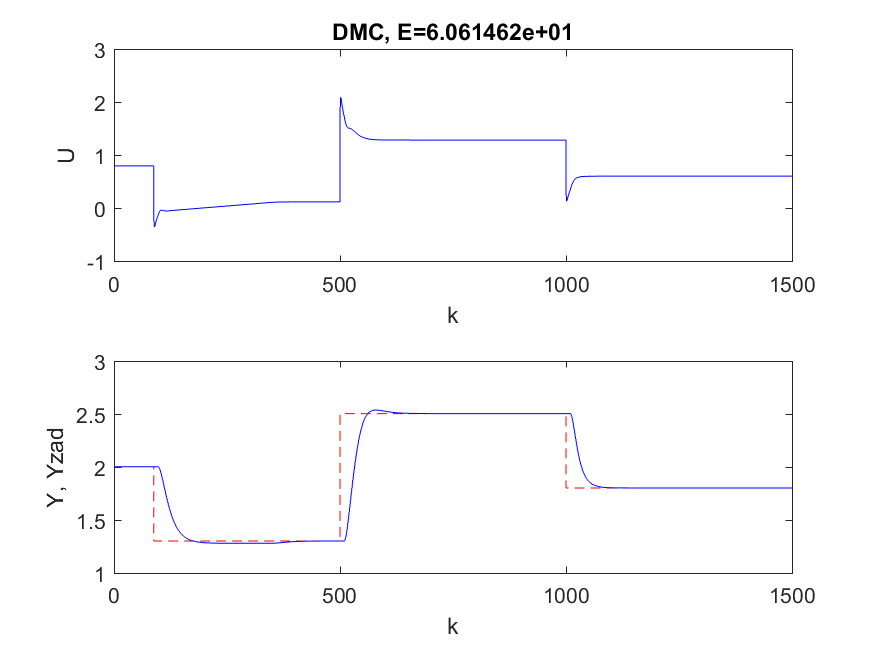
\includegraphics{dmc_inz.png}
\label{dmcinz}
\end{figure}



\section{Optymalizacja wskaźnika jakości}
Następnie dokonano optymalizacji wskaźnika jakości regulatorów PID i DMC dla tej samej trajektorii z wykorzystaniem funkcji wbudowanych w środowisku Matlab. Za przyjęty wskaźnik jakości przyjęto sumę kwadratrów róznic pomiędzy wartością zadaną, a wartością wyjścia symulowanego obiektu:

\begin{equation}
E = \sum_{k=1}^{N} (Y^{zad}(k)-Y(k))^2
\end{equation}

Dla regulatora PID do doboru optymalnych parametrów wykorzystano funkcję \verb+fmincon+ radzącą sobie z problemem optymalizacji nieliniowej. W ten sposób otrzymano wartości $K=\num{4.6203}$, $T_\mathrm{i}=\num{6.5674}$, $T_\mathrm{d}=\num{4.8067}$. Wskaźnik jakości wyniósł w tym przypadku $E=\num{66.6405}$. Jest więc on mniejszy, niż w przypadku nastaw ręcznych, dla wartości $Y_\mathrm{zad}=\num{2.5}$ pojawiły się jednak silne oscylacje. Przebiegi przedstawiono na rys.~\ref{pidoptu} i \ref{pidopty}.

W przypadku regulatora DMC ze względu na parametry $N$, $N_u$ przyjmujące wartości całkowite należało zastosować funkcję umożliwiającą optymalizację wskaźnika jakości dla parametrów o wartościach całkowitych. W tym celu wykorzystano funkcję \verb+ga+, czyli funkcję wykorzystującą algorytm genetyczny do optymalizacji. W ten sposób otrzymano parametry $N=43$, $N_\mathrm{u}=1$, $\lambda=\num{1.0555}$. Wskaźnik jakości dla tych parametrów wynosi $E=\num{60.369}$. Wyniki symulacji z takimi parametrami znajdują się na rys.~\ref{dmcopt}



\begin{figure}

	\centering
	\caption{Przebieg symulacji PID dla parametrów dobranych poprzez optymalizację wskaźnika jakości - wartość sygnału sterującego}
	% This file was created by matlab2tikz.
%
\definecolor{mycolor1}{rgb}{1.00000,0.00000,1.00000}%
%
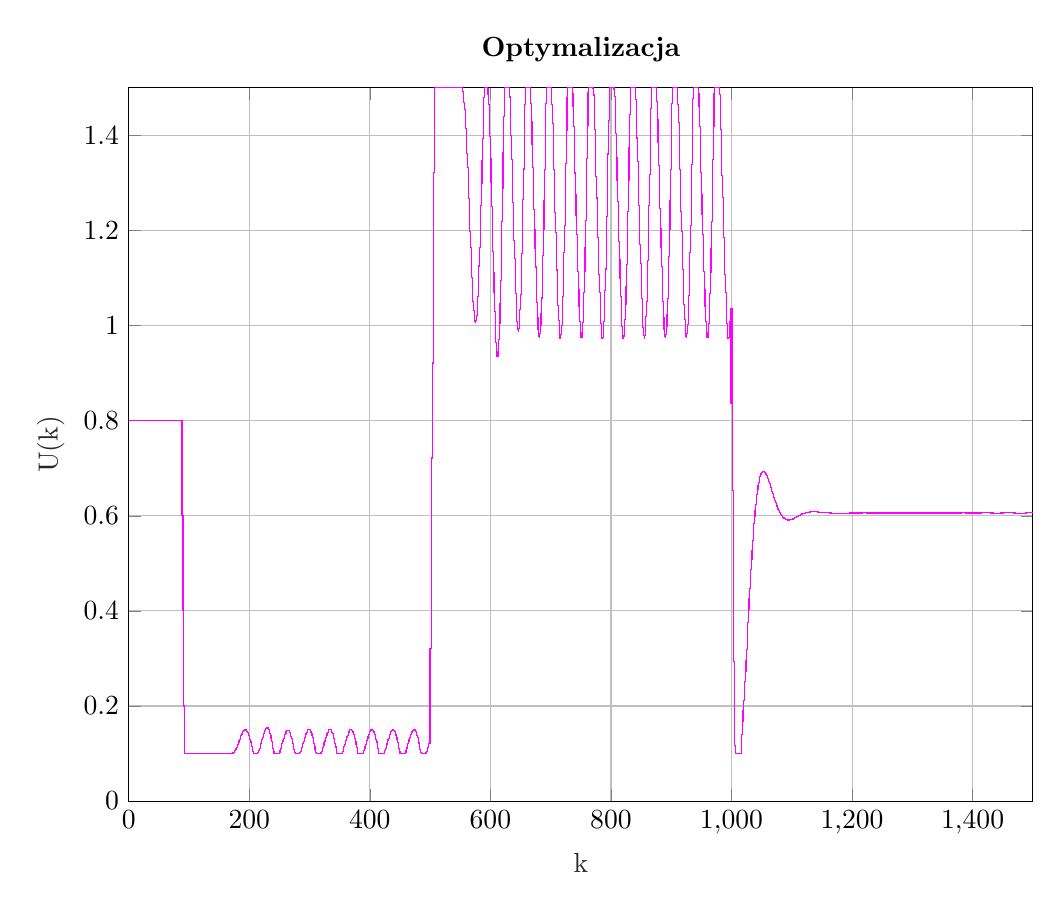
\begin{tikzpicture}

\begin{axis}[%
width=4.521in,
height=3.566in,
at={(0.758in,0.481in)},
scale only axis,
xmin=0,
xmax=1500,
xlabel style={font=\color{white!15!black}},
xlabel={k},
ymin=0,
ymax=1.5,
ylabel style={font=\color{white!15!black}},
ylabel={U(k)},
axis background/.style={fill=white},
title style={font=\bfseries},
title={Optymalizacja},
xmajorgrids,
ymajorgrids,
legend style={legend cell align=left, align=left, draw=white!15!black}
]
\addplot[const plot, color=mycolor1] table[row sep=crcr] {%
0	0.8\\
1	0.8\\
2	0.8\\
3	0.8\\
4	0.8\\
5	0.8\\
6	0.8\\
7	0.8\\
8	0.8\\
9	0.8\\
10	0.8\\
11	0.8\\
12	0.8\\
13	0.8\\
14	0.8\\
15	0.8\\
16	0.8\\
17	0.8\\
18	0.8\\
19	0.8\\
20	0.8\\
21	0.8\\
22	0.8\\
23	0.8\\
24	0.8\\
25	0.8\\
26	0.8\\
27	0.8\\
28	0.8\\
29	0.8\\
30	0.8\\
31	0.8\\
32	0.8\\
33	0.8\\
34	0.8\\
35	0.8\\
36	0.8\\
37	0.8\\
38	0.8\\
39	0.8\\
40	0.8\\
41	0.8\\
42	0.8\\
43	0.8\\
44	0.8\\
45	0.8\\
46	0.8\\
47	0.8\\
48	0.8\\
49	0.8\\
50	0.8\\
51	0.8\\
52	0.8\\
53	0.8\\
54	0.8\\
55	0.8\\
56	0.8\\
57	0.8\\
58	0.8\\
59	0.8\\
60	0.8\\
61	0.8\\
62	0.8\\
63	0.8\\
64	0.8\\
65	0.8\\
66	0.8\\
67	0.8\\
68	0.8\\
69	0.8\\
70	0.8\\
71	0.8\\
72	0.8\\
73	0.8\\
74	0.8\\
75	0.8\\
76	0.8\\
77	0.8\\
78	0.8\\
79	0.8\\
80	0.8\\
81	0.8\\
82	0.8\\
83	0.8\\
84	0.8\\
85	0.8\\
86	0.8\\
87	0.6\\
88	0.8\\
89	0.6\\
90	0.4\\
91	0.2\\
92	0.1\\
93	0.1\\
94	0.1\\
95	0.1\\
96	0.1\\
97	0.1\\
98	0.1\\
99	0.1\\
100	0.1\\
101	0.1\\
102	0.1\\
103	0.1\\
104	0.1\\
105	0.1\\
106	0.1\\
107	0.1\\
108	0.1\\
109	0.1\\
110	0.1\\
111	0.1\\
112	0.1\\
113	0.1\\
114	0.1\\
115	0.1\\
116	0.1\\
117	0.1\\
118	0.1\\
119	0.1\\
120	0.1\\
121	0.1\\
122	0.1\\
123	0.1\\
124	0.1\\
125	0.1\\
126	0.1\\
127	0.1\\
128	0.1\\
129	0.1\\
130	0.1\\
131	0.1\\
132	0.1\\
133	0.1\\
134	0.1\\
135	0.1\\
136	0.1\\
137	0.1\\
138	0.1\\
139	0.1\\
140	0.1\\
141	0.1\\
142	0.1\\
143	0.1\\
144	0.1\\
145	0.1\\
146	0.1\\
147	0.1\\
148	0.1\\
149	0.1\\
150	0.1\\
151	0.1\\
152	0.1\\
153	0.1\\
154	0.1\\
155	0.1\\
156	0.1\\
157	0.1\\
158	0.1\\
159	0.1\\
160	0.1\\
161	0.1\\
162	0.1\\
163	0.1\\
164	0.1\\
165	0.1\\
166	0.1\\
167	0.1\\
168	0.1\\
169	0.1\\
170	0.1\\
171	0.100120626226829\\
172	0.100628896314545\\
173	0.101504987532028\\
174	0.102730042210163\\
175	0.104286125643467\\
176	0.106156185312348\\
177	0.108324011445328\\
178	0.110774198930961\\
179	0.113492110580832\\
180	0.116463841737664\\
181	0.119676186216851\\
182	0.123100473793641\\
183	0.126658368356215\\
184	0.130243742832328\\
185	0.133759767609951\\
186	0.13711764661026\\
187	0.140235515232701\\
188	0.143037481542055\\
189	0.145452794052331\\
190	0.147415121245882\\
191	0.148861929568963\\
192	0.149733948084043\\
193	0.149976866074398\\
194	0.149549618220774\\
195	0.148433764805208\\
196	0.14663481691935\\
197	0.144179119472392\\
198	0.141111336988256\\
199	0.137492444657484\\
200	0.133398141200572\\
201	0.128917612296691\\
202	0.12415258387416\\
203	0.119216613660562\\
204	0.114234288832622\\
205	0.109339159851343\\
206	0.104669474251254\\
207	0.100362728918221\\
208	0.1\\
209	0.1\\
210	0.1\\
211	0.1\\
212	0.1\\
213	0.100181948369816\\
214	0.101336339896159\\
215	0.103466683355667\\
216	0.106549250446438\\
217	0.110532032285151\\
218	0.115334836245008\\
219	0.120389334868952\\
220	0.125180372991827\\
221	0.129718348575399\\
222	0.134055026366292\\
223	0.138235748552387\\
224	0.142275797357497\\
225	0.146057628816397\\
226	0.149364936977493\\
227	0.151989909311459\\
228	0.153738780971855\\
229	0.154437413028102\\
230	0.15399829822152\\
231	0.152470807902152\\
232	0.14995796210081\\
233	0.146542635239102\\
234	0.14228525801639\\
235	0.137230675328704\\
236	0.131431254381522\\
237	0.124977318772432\\
238	0.118007580394712\\
239	0.11070496618201\\
240	0.103291453336969\\
241	0.1\\
242	0.1\\
243	0.1\\
244	0.1\\
245	0.1\\
246	0.1\\
247	0.1\\
248	0.1\\
249	0.10062057488062\\
250	0.102778787305945\\
251	0.106492586149257\\
252	0.111194414777222\\
253	0.11592457854839\\
254	0.120316158854673\\
255	0.124433993058951\\
256	0.128334985108577\\
257	0.132068955936934\\
258	0.135679407762795\\
259	0.139204210763013\\
260	0.142593238394031\\
261	0.145594188010698\\
262	0.147843925829055\\
263	0.149064300295317\\
264	0.149182918639344\\
265	0.148293004126093\\
266	0.14651302015925\\
267	0.143932934264526\\
268	0.140618726994143\\
269	0.136616255613384\\
270	0.131954558955945\\
271	0.126659774906696\\
272	0.120794022548175\\
273	0.114494789950703\\
274	0.10797500152403\\
275	0.101482536839299\\
276	0.1\\
277	0.1\\
278	0.1\\
279	0.1\\
280	0.1\\
281	0.1\\
282	0.1\\
283	0.1\\
284	0.101312228844446\\
285	0.104011198829111\\
286	0.108088373876498\\
287	0.112846128925745\\
288	0.117464604321143\\
289	0.121808880211949\\
290	0.125934761952451\\
291	0.129891138123504\\
292	0.133720725675623\\
293	0.137460739448957\\
294	0.141143493522979\\
295	0.144621473892569\\
296	0.147574551193594\\
297	0.14968501501282\\
298	0.150738158763548\\
299	0.150719671759152\\
300	0.14972960598422\\
301	0.147865214500964\\
302	0.145198964906953\\
303	0.141782473461123\\
304	0.137649876322121\\
305	0.132820713291453\\
306	0.127325852837073\\
307	0.121253384189442\\
308	0.114768197650073\\
309	0.108095375577611\\
310	0.10147899474138\\
311	0.1\\
312	0.1\\
313	0.1\\
314	0.1\\
315	0.1\\
316	0.1\\
317	0.1\\
318	0.1\\
319	0.101357217488789\\
320	0.104124597232429\\
321	0.10828573636499\\
322	0.113122999889403\\
323	0.117802543175693\\
324	0.122192194912685\\
325	0.126349787818739\\
326	0.130326016013221\\
327	0.134165202835275\\
328	0.137905990796465\\
329	0.141581961338259\\
330	0.145040708343932\\
331	0.147954522000523\\
332	0.150002128503198\\
333	0.150968932102441\\
334	0.150844961594723\\
335	0.149735654626792\\
336	0.14774265860579\\
337	0.144942052473914\\
338	0.141388404984845\\
339	0.137118252148734\\
340	0.132153071637908\\
341	0.126526089432944\\
342	0.120329307658902\\
343	0.113732834634125\\
344	0.1069672406651\\
345	0.100281347884392\\
346	0.1\\
347	0.1\\
348	0.1\\
349	0.1\\
350	0.1\\
351	0.1\\
352	0.1\\
353	0.100146560156946\\
354	0.101690123402069\\
355	0.104664559029475\\
356	0.109048559264299\\
357	0.113952895163598\\
358	0.118551427113608\\
359	0.122870967753432\\
360	0.126968139884054\\
361	0.130892552199861\\
362	0.134687554752184\\
363	0.138390917750139\\
364	0.14201584367729\\
365	0.145386173555417\\
366	0.148167522474809\\
367	0.150035078086035\\
368	0.150794165079903\\
369	0.150474328704758\\
370	0.149196406252724\\
371	0.147056894156055\\
372	0.144127507812746\\
373	0.14045913015135\\
374	0.136085193659527\\
375	0.131027192428837\\
376	0.125324250217788\\
377	0.119078025237237\\
378	0.112469318439799\\
379	0.105736904106754\\
380	0.1\\
381	0.1\\
382	0.1\\
383	0.1\\
384	0.1\\
385	0.1\\
386	0.1\\
387	0.1\\
388	0.100407762496374\\
389	0.102215183146423\\
390	0.105446710195094\\
391	0.109954505753337\\
392	0.114829518991106\\
393	0.119375050790278\\
394	0.12365383596518\\
395	0.127720942830407\\
396	0.131624594585671\\
397	0.135406907555811\\
398	0.139104554469265\\
399	0.142694835409128\\
400	0.145968766159664\\
401	0.148594512001911\\
402	0.15026743318028\\
403	0.150830505478874\\
404	0.150334276863872\\
405	0.148898504034014\\
406	0.146614530820356\\
407	0.143549751008465\\
408	0.13975143635001\\
409	0.135250014383059\\
410	0.130069160876846\\
411	0.124259119625475\\
412	0.117936098710608\\
413	0.111291947766988\\
414	0.104568658243921\\
415	0.1\\
416	0.1\\
417	0.1\\
418	0.1\\
419	0.1\\
420	0.1\\
421	0.1\\
422	0.1\\
423	0.100653494516346\\
424	0.102713470890937\\
425	0.106194460215385\\
426	0.1107896400463\\
427	0.115607634740596\\
428	0.12010670656965\\
429	0.124348308083954\\
430	0.128386362376963\\
431	0.132268070614031\\
432	0.136034637779356\\
433	0.139721924692223\\
434	0.143273650271981\\
435	0.146449542573647\\
436	0.148919356318659\\
437	0.150402116069217\\
438	0.150780890505334\\
439	0.150121411971954\\
440	0.148538568727012\\
441	0.146119596449527\\
442	0.142928433379711\\
443	0.139009454951479\\
444	0.134390670735328\\
445	0.129098140665993\\
446	0.12319291422277\\
447	0.116805376209299\\
448	0.110137715374359\\
449	0.103433682171886\\
450	0.1\\
451	0.1\\
452	0.1\\
453	0.1\\
454	0.1\\
455	0.1\\
456	0.1\\
457	0.1\\
458	0.100892322192678\\
459	0.103195914721115\\
460	0.106915675741115\\
461	0.111591805331545\\
462	0.116351362484104\\
463	0.120803043336873\\
464	0.125006952661717\\
465	0.12901581008275\\
466	0.132875743001781\\
467	0.136626999179093\\
468	0.140304586881043\\
469	0.143819531140902\\
470	0.146901348084423\\
471	0.149221762014436\\
472	0.150523000981603\\
473	0.150726939126492\\
474	0.149913785147079\\
475	0.148193469588079\\
476	0.145649049337026\\
477	0.142340951805056\\
478	0.138310613408684\\
479	0.133583593298606\\
480	0.128188187956234\\
481	0.122195851763892\\
482	0.115750571818852\\
483	0.10906433394329\\
484	0.102382350319334\\
485	0.1\\
486	0.1\\
487	0.1\\
488	0.1\\
489	0.1\\
490	0.1\\
491	0.1\\
492	0.1\\
493	0.101116657024439\\
494	0.103648278261501\\
495	0.107590592458193\\
496	0.11234257554007\\
497	0.117048914062143\\
498	0.121457640669384\\
499	0.321457640669384\\
500	0.121457640669384\\
501	0.321457640669384\\
502	0.521457640669384\\
503	0.721457640669384\\
504	0.921457640669384\\
505	1.12145764066938\\
506	1.32145764066938\\
507	1.5\\
508	1.5\\
509	1.5\\
510	1.5\\
511	1.5\\
512	1.5\\
513	1.5\\
514	1.5\\
515	1.5\\
516	1.5\\
517	1.5\\
518	1.5\\
519	1.5\\
520	1.5\\
521	1.5\\
522	1.5\\
523	1.5\\
524	1.5\\
525	1.5\\
526	1.5\\
527	1.5\\
528	1.5\\
529	1.5\\
530	1.5\\
531	1.5\\
532	1.5\\
533	1.5\\
534	1.5\\
535	1.5\\
536	1.5\\
537	1.5\\
538	1.5\\
539	1.5\\
540	1.5\\
541	1.5\\
542	1.5\\
543	1.5\\
544	1.5\\
545	1.5\\
546	1.5\\
547	1.5\\
548	1.5\\
549	1.5\\
550	1.5\\
551	1.5\\
552	1.5\\
553	1.49752394848959\\
554	1.49153739192139\\
555	1.48217658198253\\
556	1.46957548560446\\
557	1.4538654255147\\
558	1.4351747861622\\
559	1.41362877710955\\
560	1.38934924683006\\
561	1.36245454060504\\
562	1.33305939689896\\
563	1.30127487720173\\
564	1.2675394149231\\
565	1.23272562752229\\
566	1.19778343353792\\
567	1.16359314130212\\
568	1.13097432317281\\
569	1.1006936241286\\
570	1.07347161560891\\
571	1.04998879529986\\
572	1.03089082421307\\
573	1.01679308382443\\
574	1.00828462817604\\
575	1.0058873262955\\
576	1.0099601828191\\
577	1.02064149913049\\
578	1.03785737622728\\
579	1.0613457958827\\
580	1.09067609940502\\
581	1.12526458399735\\
582	1.16438683740108\\
583	1.2071873448441\\
584	1.25268682679661\\
585	1.29978770031455\\
586	1.34728391959723\\
587	1.39388810559387\\
588	1.43827720383004\\
589	1.47914238767334\\
590	1.5\\
591	1.5\\
592	1.5\\
593	1.5\\
594	1.5\\
595	1.49781429119282\\
596	1.48634051714852\\
597	1.46555828654024\\
598	1.43571015098391\\
599	1.39730976822152\\
600	1.35113893024246\\
601	1.300271047662\\
602	1.2498146620614\\
603	1.20195960508501\\
604	1.15617686175186\\
605	1.11200297528698\\
606	1.06932525128005\\
607	1.02929731512373\\
608	0.993958455021117\\
609	0.965266734646833\\
610	0.945045198674656\\
611	0.934928385508892\\
612	0.936039255484641\\
613	0.94845585743048\\
614	0.971392627139627\\
615	1.00396834722357\\
616	1.04553633247639\\
617	1.0956079078907\\
618	1.1536226093196\\
619	1.21866467660977\\
620	1.28936962648722\\
621	1.363962918268\\
622	1.44030838421117\\
623	1.5\\
624	1.5\\
625	1.5\\
626	1.5\\
627	1.5\\
628	1.5\\
629	1.5\\
630	1.5\\
631	1.49822252499368\\
632	1.48075243093607\\
633	1.44728623972046\\
634	1.40016721335598\\
635	1.3496319406874\\
636	1.30287195069819\\
637	1.25918347994187\\
638	1.21794836152519\\
639	1.17862487144649\\
640	1.14073950069419\\
641	1.10387956203151\\
642	1.06792422775309\\
643	1.03487664791799\\
644	1.00848850305166\\
645	0.992112433792568\\
646	0.98735157571019\\
647	0.993561654216579\\
648	1.0093995093382\\
649	1.03383544948985\\
650	1.0661039281045\\
651	1.10566125389953\\
652	1.15214939565195\\
653	1.2053332794337\\
654	1.2647681030292\\
655	1.32930015802616\\
656	1.39692357066693\\
657	1.46509225282698\\
658	1.5\\
659	1.5\\
660	1.5\\
661	1.5\\
662	1.5\\
663	1.5\\
664	1.5\\
665	1.5\\
666	1.4908230734235\\
667	1.46726106566498\\
668	1.42921548418284\\
669	1.38134830964361\\
670	1.33254411527657\\
671	1.28678846886211\\
672	1.24347713803252\\
673	1.20208037235285\\
674	1.16213489637093\\
675	1.12323671446722\\
676	1.08503464753955\\
677	1.04845163990931\\
678	1.01625923678282\\
679	0.99181339978329\\
680	0.977760409226466\\
681	0.974919473177544\\
682	0.982497049290938\\
683	0.999395036580346\\
684	1.02478651344471\\
685	1.05807290860839\\
686	1.09884728263598\\
687	1.1468629033944\\
688	1.20184231671954\\
689	1.26306438496344\\
690	1.32906586291251\\
691	1.39768711130979\\
692	1.46642495967816\\
693	1.5\\
694	1.5\\
695	1.5\\
696	1.5\\
697	1.5\\
698	1.5\\
699	1.5\\
700	1.5\\
701	1.48979234795583\\
702	1.46507398271479\\
703	1.42585594514956\\
704	1.37709556791779\\
705	1.32771415793721\\
706	1.2815020180624\\
707	1.23783987106863\\
708	1.19618454584476\\
709	1.15606080544601\\
710	1.11705400321589\\
711	1.07880348543303\\
712	1.04236160290365\\
713	1.01063394231381\\
714	0.986976407257924\\
715	0.97398409956231\\
716	0.972387089462913\\
717	0.981329831812873\\
718	0.999682811515947\\
719	1.0265933400352\\
720	1.06144182088978\\
721	1.10380425712731\\
722	1.15342016656641\\
723	1.20998266109779\\
724	1.27270783888598\\
725	1.34005499809284\\
726	1.40979646538949\\
727	1.47938113082547\\
728	1.5\\
729	1.5\\
730	1.5\\
731	1.5\\
732	1.5\\
733	1.5\\
734	1.5\\
735	1.5\\
736	1.48774257513255\\
737	1.46073261567372\\
738	1.41904016669779\\
739	1.3694937525783\\
740	1.32094206559484\\
741	1.27545377027249\\
742	1.23242112167426\\
743	1.19131130457462\\
744	1.15165837775552\\
745	1.11305603507474\\
746	1.07515110285044\\
747	1.03927672632759\\
748	1.00862485106207\\
749	0.986589010475361\\
750	0.975545827077236\\
751	0.975792082743549\\
752	0.986299312845838\\
753	1.00598840664151\\
754	1.0340494246492\\
755	1.06989892660201\\
756	1.1131434035037\\
757	1.16354799656065\\
758	1.22079062385649\\
759	1.28399797628869\\
760	1.35150154166204\\
761	1.42097443072669\\
762	1.48985411512462\\
763	1.5\\
764	1.5\\
765	1.5\\
766	1.5\\
767	1.5\\
768	1.5\\
769	1.5\\
770	1.49965771564646\\
771	1.48500974632345\\
772	1.45565943058561\\
773	1.41177441716751\\
774	1.36152711939948\\
775	1.31353036949823\\
776	1.26846899951838\\
777	1.22575151149791\\
778	1.18485957111791\\
779	1.14534013198661\\
780	1.10679835891899\\
781	1.06893704070157\\
782	1.03341367219291\\
783	1.00366575799671\\
784	0.983043798431177\\
785	0.973694541205986\\
786	0.975558879996526\\
787	0.987484391235338\\
788	1.00844562676698\\
789	1.03767768290101\\
790	1.07463478063162\\
791	1.11895477997801\\
792	1.17042271288465\\
793	1.22868413583065\\
794	1.29276008314252\\
795	1.36085476525561\\
796	1.43055432051668\\
797	1.49928756308146\\
798	1.5\\
799	1.5\\
800	1.5\\
801	1.5\\
802	1.5\\
803	1.5\\
804	1.5\\
805	1.49773602328124\\
806	1.4810500096313\\
807	1.4496211553875\\
808	1.40370187639094\\
809	1.35273925820837\\
810	1.30519365336637\\
811	1.26049858468101\\
812	1.21807289399434\\
813	1.17740748018976\\
814	1.13805753543433\\
815	1.09963556940064\\
816	1.06210787585926\\
817	1.02738584798553\\
818	0.998911543919579\\
819	0.980021771765822\\
820	0.972671749706827\\
821	0.976480411684791\\
822	0.99017541578948\\
823	1.01277296653157\\
824	1.04354335895115\\
825	1.08197046289926\\
826	1.12771702241622\\
827	1.18055450925734\\
828	1.24004716191737\\
829	1.30510446924814\\
830	1.37382381654334\\
831	1.44371445798145\\
832	1.5\\
833	1.5\\
834	1.5\\
835	1.5\\
836	1.5\\
837	1.5\\
838	1.5\\
839	1.5\\
840	1.4951616905277\\
841	1.47577486663643\\
842	1.44161020960462\\
843	1.3946497392296\\
844	1.34428440968606\\
845	1.29731294466428\\
846	1.25308761479923\\
847	1.21103988748348\\
848	1.17067194003996\\
849	1.13154903205785\\
850	1.09329265232714\\
851	1.05622132797267\\
852	1.02258197386895\\
853	0.99581602081412\\
854	0.979020718297976\\
855	0.973713994504049\\
856	0.979328121087294\\
857	0.994632969861333\\
858	1.01869118772626\\
859	1.05081217756501\\
860	1.09051262811428\\
861	1.13748271953496\\
862	1.19147073168752\\
863	1.25192822748638\\
864	1.31761348413412\\
865	1.38650978495336\\
866	1.45610359981838\\
867	1.5\\
868	1.5\\
869	1.5\\
870	1.5\\
871	1.5\\
872	1.5\\
873	1.5\\
874	1.5\\
875	1.49252357610494\\
876	1.47046190002582\\
877	1.43369175303148\\
878	1.38585397881387\\
879	1.33612756085578\\
880	1.28966987978072\\
881	1.2458485912618\\
882	1.20410889543809\\
883	1.16396521753024\\
884	1.12499373112946\\
885	1.08682564119512\\
886	1.05014087641055\\
887	1.01751814374658\\
888	0.992373242470776\\
889	0.977547561173625\\
890	0.974135798236865\\
891	0.981413780628321\\
892	0.998206787895219\\
893	1.02362413206192\\
894	1.05701438848254\\
895	1.09792700829388\\
896	1.14607946040916\\
897	1.20119547863257\\
898	1.26261209016478\\
899	1.32893848396159\\
900	1.39805128984875\\
901	1.46742157374931\\
902	1.5\\
903	1.5\\
904	1.5\\
905	1.5\\
906	1.5\\
907	1.5\\
908	1.5\\
909	1.5\\
910	1.49010489951832\\
911	1.46558218096709\\
912	1.42640806782222\\
913	1.3777458629785\\
914	1.32858637161555\\
915	1.28258673015087\\
916	1.23912792619298\\
917	1.19766706237074\\
918	1.15772918169602\\
919	1.11889992135099\\
920	1.08081891331688\\
921	1.04449700078904\\
922	1.01281786934495\\
923	0.989175408810923\\
924	0.976177489749405\\
925	0.97453081156758\\
926	0.983366449633236\\
927	1.00155879058376\\
928	1.02825853915476\\
929	1.06284904747532\\
930	1.10490887937989\\
931	1.15417977620889\\
932	1.21036236949486\\
933	1.27268804792468\\
934	1.33962838802496\\
935	1.40896099497301\\
936	1.47814146654406\\
937	1.5\\
938	1.5\\
939	1.5\\
940	1.5\\
941	1.5\\
942	1.5\\
943	1.5\\
944	1.5\\
945	1.4878341149978\\
946	1.46099673709632\\
947	1.41955653198221\\
948	1.37012111636394\\
949	1.32150599096814\\
950	1.27594732503311\\
951	1.23283873397961\\
952	1.19164859560596\\
953	1.15191201235808\\
954	1.1132235885502\\
955	1.07523094225952\\
956	1.03925566439133\\
957	1.00846837994288\\
958	0.986243631127912\\
959	0.974969335767106\\
960	0.974985165472356\\
961	0.98528515965471\\
962	1.00479027567444\\
963	1.03269047538214\\
964	1.06840209568334\\
965	1.11153131520059\\
966	1.16184290106172\\
967	1.21901599451596\\
968	1.28218289871494\\
969	1.34968583586527\\
970	1.41920922837545\\
971	1.48819440228437\\
972	1.5\\
973	1.5\\
974	1.5\\
975	1.5\\
976	1.5\\
977	1.5\\
978	1.5\\
979	1.49999984682356\\
980	1.48569700124513\\
981	1.45668459522957\\
982	1.41311842011165\\
983	1.36295837937522\\
984	1.3148533980514\\
985	1.26970720788142\\
986	1.22692537425688\\
987	1.18598694402643\\
988	1.14643653745625\\
989	1.10787724237538\\
990	1.06996425194937\\
991	1.03431162366193\\
992	1.00435959040176\\
993	0.983463674707136\\
994	0.973804929966184\\
995	0.975378831232792\\
996	0.987051159639405\\
997	1.0077867518492\\
998	1.03681255200943\\
999	0.836812552009434\\
1000	1.03681255200943\\
1001	0.841870314603431\\
1002	0.653743234418035\\
1003	0.471470424327802\\
1004	0.293272594615016\\
1005	0.116746775933597\\
1006	0.1\\
1007	0.1\\
1008	0.1\\
1009	0.1\\
1010	0.1\\
1011	0.1\\
1012	0.1\\
1013	0.1\\
1014	0.1\\
1015	0.1\\
1016	0.110416545836438\\
1017	0.140133350212443\\
1018	0.167022270254366\\
1019	0.190376176986272\\
1020	0.211526941148046\\
1021	0.23162588833363\\
1022	0.251663890511138\\
1023	0.272489387890288\\
1024	0.294824546658854\\
1025	0.319279738084069\\
1026	0.346366506380557\\
1027	0.375116307703831\\
1028	0.402035490957854\\
1029	0.425555887742373\\
1030	0.447002034698933\\
1031	0.467464335697441\\
1032	0.487589163453051\\
1033	0.507655403231618\\
1034	0.527639230947571\\
1035	0.547268797966585\\
1036	0.566070273098043\\
1037	0.583406498233769\\
1038	0.598695594676204\\
1039	0.611933866788878\\
1040	0.623733398179265\\
1041	0.634667506267554\\
1042	0.644944638872325\\
1043	0.654521190165655\\
1044	0.663222849529414\\
1045	0.670840190691133\\
1046	0.67720339571834\\
1047	0.682240170371769\\
1048	0.686020201057175\\
1049	0.688764004966059\\
1050	0.690754489482198\\
1051	0.692181829496829\\
1052	0.693078158769512\\
1053	0.693380971292318\\
1054	0.693018707186872\\
1055	0.691961157879116\\
1056	0.690239237176149\\
1057	0.687941895275634\\
1058	0.685196218497544\\
1059	0.682135364479674\\
1060	0.678861199846184\\
1061	0.675419187209272\\
1062	0.671806001017107\\
1063	0.668004722281122\\
1064	0.664017850399207\\
1065	0.659879185114581\\
1066	0.655647643957017\\
1067	0.651392465030706\\
1068	0.647177080653341\\
1069	0.643046771150006\\
1070	0.639023587437831\\
1071	0.635110397810254\\
1072	0.631302666349157\\
1073	0.627601728884929\\
1074	0.624021748805847\\
1075	0.620587522311933\\
1076	0.617326693296062\\
1077	0.614261710558932\\
1078	0.611404932354332\\
1079	0.608757958140459\\
1080	0.606314634702165\\
1081	0.604066123015836\\
1082	0.602005817639071\\
1083	0.600131971828293\\
1084	0.598446984470237\\
1085	0.596954170738479\\
1086	0.59565414905999\\
1087	0.594542748252101\\
1088	0.593611087037267\\
1089	0.592847327953799\\
1090	0.592239068268504\\
1091	0.591775324543788\\
1092	0.591447403409178\\
1093	0.591248478980649\\
1094	0.591172264428736\\
1095	0.591211550924922\\
1096	0.591357369306397\\
1097	0.591599106100286\\
1098	0.591925370053222\\
1099	0.592325092112883\\
1100	0.592788353583436\\
1101	0.593306662857773\\
1102	0.593872682567843\\
1103	0.594479631962519\\
1104	0.595120689342517\\
1105	0.595788673817019\\
1106	0.596476120849635\\
1107	0.597175663914552\\
1108	0.597880501050373\\
1109	0.598584722192237\\
1110	0.599283378663198\\
1111	0.599972313662421\\
1112	0.60064787150377\\
1113	0.601306631802592\\
1114	0.60194527731885\\
1115	0.602560627691372\\
1116	0.603149792350036\\
1117	0.603710348453456\\
1118	0.604240451955158\\
1119	0.604738834900178\\
1120	0.605204701762553\\
1121	0.605637580650844\\
1122	0.606037194658527\\
1123	0.606403397395205\\
1124	0.606736180531041\\
1125	0.607035728283762\\
1126	0.607302477353173\\
1127	0.607537145183923\\
1128	0.60774070968544\\
1129	0.60791434835009\\
1130	0.608059362007873\\
1131	0.608177111352166\\
1132	0.608268983985536\\
1133	0.608336393278304\\
1134	0.608380796360497\\
1135	0.608403712750957\\
1136	0.608406728465088\\
1137	0.608391479871217\\
1138	0.608359621968045\\
1139	0.608312792395279\\
1140	0.608252582980178\\
1141	0.608180525706901\\
1142	0.608098092793843\\
1143	0.60800670474508\\
1144	0.607907738191848\\
1145	0.607802527290191\\
1146	0.607692356795922\\
1147	0.607578449347625\\
1148	0.607461952004854\\
1149	0.607343926923333\\
1150	0.607225348717238\\
1151	0.60710710795395\\
1152	0.60699001787031\\
1153	0.606874820727636\\
1154	0.606762191251639\\
1155	0.6066527365729\\
1156	0.606546993947726\\
1157	0.606445428487003\\
1158	0.606348432893443\\
1159	0.606256330109745\\
1160	0.606169378447516\\
1161	0.606087777831582\\
1162	0.606011675608412\\
1163	0.605941170889029\\
1164	0.605876317274049\\
1165	0.605817124587531\\
1166	0.60576356059715\\
1167	0.605715553538979\\
1168	0.605672995757282\\
1169	0.605635748200578\\
1170	0.60560364514945\\
1171	0.605576498518371\\
1172	0.605554101331968\\
1173	0.605536230363289\\
1174	0.605522648242679\\
1175	0.605513105470518\\
1176	0.605507342673248\\
1177	0.605505093210533\\
1178	0.605506085999866\\
1179	0.6055100482831\\
1180	0.605516708064756\\
1181	0.605525796075812\\
1182	0.605537047285805\\
1183	0.605550202115802\\
1184	0.60556500754593\\
1185	0.605581218259385\\
1186	0.605598597859988\\
1187	0.605616920098192\\
1188	0.605635969986361\\
1189	0.605655544693857\\
1190	0.605675454171068\\
1191	0.605695521523981\\
1192	0.605715583213328\\
1193	0.605735489164124\\
1194	0.605755102844702\\
1195	0.605774301327775\\
1196	0.605792975303671\\
1197	0.605811028996133\\
1198	0.605828379939175\\
1199	0.605844958601027\\
1200	0.605860707873008\\
1201	0.605875582462228\\
1202	0.60588954823051\\
1203	0.605902581508933\\
1204	0.605914668397451\\
1205	0.605925804041809\\
1206	0.605935991873592\\
1207	0.605945242804099\\
1208	0.605953574375753\\
1209	0.605961009888091\\
1210	0.605967577523521\\
1211	0.605973309498028\\
1212	0.605978241255371\\
1213	0.605982410713705\\
1214	0.60598585756573\\
1215	0.605988622630426\\
1216	0.605990747255881\\
1217	0.60599227277736\\
1218	0.605993240038993\\
1219	0.605993688989233\\
1220	0.605993658358066\\
1221	0.605993185419714\\
1222	0.605992305838525\\
1223	0.605991053591617\\
1224	0.60598946095927\\
1225	0.605987558574098\\
1226	0.605985375521036\\
1227	0.605982939481379\\
1228	0.605980276914157\\
1229	0.605977413267029\\
1230	0.605974373206838\\
1231	0.605971180857966\\
1232	0.605967860035562\\
1233	0.605964434460754\\
1234	0.605960927946363\\
1235	0.605957364543529\\
1236	0.605953768641958\\
1237	0.605950165018247\\
1238	0.605946578828311\\
1239	0.605943035540938\\
1240	0.605939560811021\\
1241	0.605936180292441\\
1242	0.60593291939279\\
1243	0.605929802974503\\
1244	0.605926855009625\\
1245	0.60592409819741\\
1246	0.605921553556122\\
1247	0.605919240001373\\
1248	0.605917173924373\\
1249	0.605915368783674\\
1250	0.605913834724496\\
1251	0.605912578239267\\
1252	0.60591160188308\\
1253	0.605910904056824\\
1254	0.605910478869723\\
1255	0.605910316091088\\
1256	0.605910401199228\\
1257	0.60591071553266\\
1258	0.605911236545945\\
1259	0.605911938169656\\
1260	0.605912791270816\\
1261	0.605913764207146\\
1262	0.605914823465698\\
1263	0.605915934373438\\
1264	0.605917061864687\\
1265	0.605918171288005\\
1266	0.605919229233049\\
1267	0.605920204356278\\
1268	0.605921068183421\\
1269	0.60592179586628\\
1270	0.605922366871548\\
1271	0.605922765580302\\
1272	0.605922981778341\\
1273	0.605923011019619\\
1274	0.60592285484776\\
1275	0.60592252086385\\
1276	0.605922022632417\\
1277	0.60592137942176\\
1278	0.605920615778992\\
1279	0.605919760945072\\
1280	0.605918848119563\\
1281	0.605917913589633\\
1282	0.605916995742098\\
1283	0.605916133981433\\
1284	0.605915367580362\\
1285	0.605914734492316\\
1286	0.605914270157746\\
1287	0.605914006337567\\
1288	0.605913970007692\\
1289	0.605914182348388\\
1290	0.605914657860819\\
1291	0.605915403641128\\
1292	0.605916418839021\\
1293	0.605917694323825\\
1294	0.605919212576195\\
1295	0.605920947817807\\
1296	0.605922866385426\\
1297	0.605924927348876\\
1298	0.605927083365657\\
1299	0.605929281757833\\
1300	0.605931465790001\\
1301	0.60593357612046\\
1302	0.605935552391581\\
1303	0.605937334920136\\
1304	0.605938866443498\\
1305	0.605940093874501\\
1306	0.605940970015242\\
1307	0.60594145517918\\
1308	0.605941518671332\\
1309	0.605941140078218\\
1310	0.605940310322478\\
1311	0.60593903244191\\
1312	0.605937322058576\\
1313	0.60593520751116\\
1314	0.60593272963196\\
1315	0.605929941159278\\
1316	0.605926905785953\\
1317	0.605923696854983\\
1318	0.605920395723876\\
1319	0.605917089829572\\
1320	0.6059138704957\\
1321	0.60591083053308\\
1322	0.605908061692464\\
1323	0.605905652035213\\
1324	0.605903683292912\\
1325	0.605902228290178\\
1326	0.605901348506551\\
1327	0.605901091852542\\
1328	0.60590149073223\\
1329	0.605902560459775\\
1330	0.605904298090145\\
1331	0.605906681715262\\
1332	0.60590967026571\\
1333	0.605913203845762\\
1334	0.605917204615349\\
1335	0.605921578217842\\
1336	0.605926215737042\\
1337	0.605930996150906\\
1338	0.605935789234076\\
1339	0.605940458846703\\
1340	0.605944866533043\\
1341	0.605948875341504\\
1342	0.605952353767524\\
1343	0.60595517971292\\
1344	0.60595724435047\\
1345	0.605958455779869\\
1346	0.605958742362768\\
1347	0.605958055628285\\
1348	0.605956372648149\\
1349	0.605953697791144\\
1350	0.605950063780256\\
1351	0.605945531992253\\
1352	0.605940191958445\\
1353	0.605934160045946\\
1354	0.605927577321358\\
1355	0.605920606621876\\
1356	0.60591342888242\\
1357	0.605906238790527\\
1358	0.605899239862961\\
1359	0.605892639058448\\
1360	0.605886641059087\\
1361	0.605881442367971\\
1362	0.605877225382425\\
1363	0.605874152609704\\
1364	0.605872361195188\\
1365	0.605871957931774\\
1366	0.60587301491275\\
1367	0.605875565979313\\
1368	0.605879604097807\\
1369	0.605885079781583\\
1370	0.605891900647338\\
1371	0.605899932167988\\
1372	0.605908999652594\\
1373	0.605918891450555\\
1374	0.605929363342527\\
1375	0.605940144045076\\
1376	0.605950941721542\\
1377	0.60596145135835\\
1378	0.605971362835206\\
1379	0.605980369490827\\
1380	0.605988176962824\\
1381	0.605994512063307\\
1382	0.605999131440121\\
1383	0.606001829769101\\
1384	0.606002447224692\\
1385	0.606000875985968\\
1386	0.605997065551786\\
1387	0.605991026662698\\
1388	0.605982833657945\\
1389	0.60597262513275\\
1390	0.605960602803489\\
1391	0.605947028534946\\
1392	0.605932219534102\\
1393	0.605916541766963\\
1394	0.605900401707767\\
1395	0.605884236581872\\
1396	0.605868503313429\\
1397	0.605853666434661\\
1398	0.605840185254307\\
1399	0.605828500616569\\
1400	0.605819021607997\\
1401	0.605812112586703\\
1402	0.605808080915505\\
1403	0.605807165777046\\
1404	0.605809528434926\\
1405	0.605815244279624\\
1406	0.605824296962017\\
1407	0.605836574871628\\
1408	0.605851870161004\\
1409	0.605869880454738\\
1410	0.605890213311096\\
1411	0.605912393429632\\
1412	0.605935872519696\\
1413	0.605960041665893\\
1414	0.60598424594853\\
1415	0.606007801002776\\
1416	0.606030011131544\\
1417	0.606050188526317\\
1418	0.606067673099498\\
1419	0.606081852392758\\
1420	0.60609218100069\\
1421	0.606098198938326\\
1422	0.606099548386028\\
1423	0.60609598826702\\
1424	0.606087406150133\\
1425	0.606073827024371\\
1426	0.606055418560807\\
1427	0.606032492560067\\
1428	0.606005502378599\\
1429	0.605975036232143\\
1430	0.60594180638683\\
1431	0.605906634365742\\
1432	0.605870432416802\\
1433	0.605834181604931\\
1434	0.605798907002309\\
1435	0.605765650553997\\
1436	0.605735442286494\\
1437	0.605709270603284\\
1438	0.605688052469314\\
1439	0.605672604324433\\
1440	0.605663614581671\\
1441	0.605661618558424\\
1442	0.605666976656712\\
1443	0.605679856551823\\
1444	0.605700220068212\\
1445	0.605727815318194\\
1446	0.605762174554827\\
1447	0.605802618047991\\
1448	0.605848264135649\\
1449	0.605898045433553\\
1450	0.605950731011861\\
1451	0.606004954169314\\
1452	0.606059245261226\\
1453	0.606112068870604\\
1454	0.606161864457921\\
1455	0.606207089488647\\
1456	0.606246263924263\\
1457	0.606278014875272\\
1458	0.606301120157971\\
1459	0.606314549473134\\
1460	0.606317501936455\\
1461	0.606309438738876\\
1462	0.606290109799651\\
1463	0.606259573396038\\
1464	0.606218207908219\\
1465	0.606166715004134\\
1466	0.606106113802077\\
1467	0.60603772578449\\
1468	0.605963150488677\\
1469	0.605884232262556\\
1470	0.605803018639235\\
1471	0.605721711145835\\
1472	0.605642609611731\\
1473	0.605568051271869\\
1474	0.605500346164589\\
1475	0.605441710493519\\
1476	0.605394199753308\\
1477	0.605359643503909\\
1478	0.605339583713268\\
1479	0.605335218570426\\
1480	0.605347353598945\\
1481	0.605376361772958\\
1482	0.605422154157091\\
1483	0.605484162359418\\
1484	0.605561333807879\\
1485	0.605652140541044\\
1486	0.605754601851285\\
1487	0.605866320740605\\
1488	0.605984533756037\\
1489	0.606106173373942\\
1490	0.606227941710517\\
1491	0.606346393962002\\
1492	0.606458029632963\\
1493	0.60655938930591\\
1494	0.606647154450964\\
1495	0.606718247579563\\
1496	0.606769929919023\\
1497	0.606799893732819\\
1498	0.606806346437792\\
1499	0.606788083778529\\
};

\end{axis}
\end{tikzpicture}%
		\label{pidoptu}
\end{figure}

\begin{figure}

	\centering
	\caption{Przebieg symulacji PID dla parametrów dobranych poprzez optymalizację wskaźnika jakości - wartość wyjścia}
	% This file was created by matlab2tikz.
%
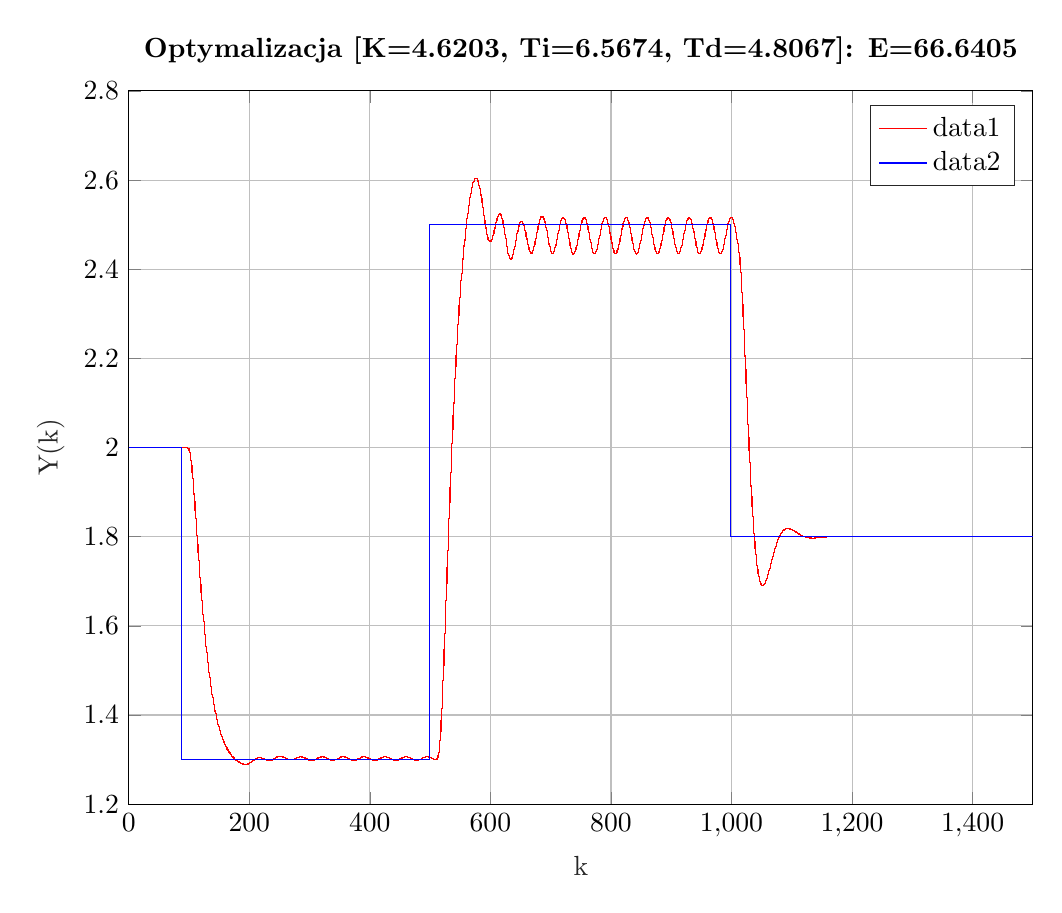
\begin{tikzpicture}

\begin{axis}[%
width=4.521in,
height=3.566in,
at={(0.758in,0.481in)},
scale only axis,
xmin=0,
xmax=1500,
xlabel style={font=\color{white!15!black}},
xlabel={k},
ymin=1.2,
ymax=2.8,
ylabel style={font=\color{white!15!black}},
ylabel={Y(k)},
axis background/.style={fill=white},
title style={font=\bfseries},
title={Optymalizacja [K=4.6203, Ti=6.5674, Td=4.8067]: E=66.6405},
xmajorgrids,
ymajorgrids,
legend style={legend cell align=left, align=left, draw=white!15!black}
]
\addplot[const plot, color=red] table[row sep=crcr] {%
0	2\\
1	2\\
2	2\\
3	2\\
4	2\\
5	2\\
6	2\\
7	2\\
8	2\\
9	2\\
10	2\\
11	2\\
12	2\\
13	2\\
14	2\\
15	2\\
16	2\\
17	2\\
18	2\\
19	2\\
20	2\\
21	2\\
22	2\\
23	2\\
24	2\\
25	2\\
26	2\\
27	2\\
28	2\\
29	2\\
30	2\\
31	2\\
32	2\\
33	2\\
34	2\\
35	2\\
36	2\\
37	2\\
38	2\\
39	2\\
40	2\\
41	2\\
42	2\\
43	2\\
44	2\\
45	2\\
46	2\\
47	2\\
48	2\\
49	2\\
50	2\\
51	2\\
52	2\\
53	2\\
54	2\\
55	2\\
56	2\\
57	2\\
58	2\\
59	2\\
60	2\\
61	2\\
62	2\\
63	2\\
64	2\\
65	2\\
66	2\\
67	2\\
68	2\\
69	2\\
70	2\\
71	2\\
72	2\\
73	2\\
74	2\\
75	2\\
76	2\\
77	2\\
78	2\\
79	2\\
80	2\\
81	2\\
82	2\\
83	2\\
84	2\\
85	2\\
86	2\\
87	2\\
88	2\\
89	2\\
90	2\\
91	2\\
92	2\\
93	2\\
94	2\\
95	2\\
96	2\\
97	1.99945658\\
98	1.998478278264\\
99	1.99710531232581\\
100	1.99434221455532\\
101	1.98934406966684\\
102	1.9816708790129\\
103	1.97148946988644\\
104	1.95921350868352\\
105	1.94520783501687\\
106	1.92979362042664\\
107	1.91325300838129\\
108	1.89583328644411\\
109	1.87775063655688\\
110	1.8591935049405\\
111	1.84032562908938\\
112	1.82128875569986\\
113	1.80220508008653\\
114	1.78317943467042\\
115	1.76430125143874\\
116	1.74564632085102\\
117	1.7272783674746\\
118	1.70925046065276\\
119	1.69160627671993\\
120	1.67438122766211\\
121	1.65760346966139\\
122	1.64129480364418\\
123	1.62547147876269\\
124	1.61014490866278\\
125	1.59532230942094\\
126	1.58100726715545\\
127	1.56720024252555\\
128	1.55389901861726\\
129	1.5410990980695\\
130	1.52879405471177\\
131	1.51697584445894\\
132	1.50563507973461\\
133	1.49476127126663\\
134	1.48434304071224\\
135	1.47436830722226\\
136	1.46482445073972\\
137	1.45569845454525\\
138	1.44697702930619\\
139	1.43864672065644\\
140	1.4306940021266\\
141	1.42310535505724\\
142	1.41586733695969\\
143	1.40896663963731\\
144	1.40239013824345\\
145	1.39612493232982\\
146	1.39015837982793\\
147	1.38447812480715\\
148	1.37907211976315\\
149	1.37392864311021\\
150	1.3690363124783\\
151	1.36438409435109\\
152	1.35996131052232\\
153	1.35575764179584\\
154	1.35176312930727\\
155	1.34796817380316\\
156	1.34436353317562\\
157	1.34094031851636\\
158	1.33768998892375\\
159	1.33460434526917\\
160	1.33167552310479\\
161	1.32889598487266\\
162	1.326258511556\\
163	1.32375619389594\\
164	1.32138242328136\\
165	1.31913088240585\\
166	1.3169955357733\\
167	1.31497062012277\\
168	1.31305063483341\\
169	1.3112303323618\\
170	1.30950470875591\\
171	1.30786899428368\\
172	1.3063186442077\\
173	1.30484932973244\\
174	1.30345692914566\\
175	1.3021375191716\\
176	1.30088736654986\\
177	1.29970291985075\\
178	1.29858080153507\\
179	1.29751780026407\\
180	1.2965108634628\\
181	1.29555741789245\\
182	1.29465635052871\\
183	1.29380843891601\\
184	1.29301597243874\\
185	1.29228242537872\\
186	1.29161217575977\\
187	1.29101026461589\\
188	1.29048219089191\\
189	1.29003373769948\\
190	1.28967082611345\\
191	1.28939939310875\\
192	1.28922524678469\\
193	1.28915376826654\\
194	1.28918945510717\\
195	1.28933548857462\\
196	1.28959341585555\\
197	1.28996292599807\\
198	1.29044170179311\\
199	1.29102533268151\\
200	1.29170727623818\\
201	1.29247885788483\\
202	1.29332930026617\\
203	1.29424578109678\\
204	1.29521354197085\\
205	1.29621608709511\\
206	1.2972354857686\\
207	1.29825275705854\\
208	1.29924830798132\\
209	1.30020240328368\\
210	1.30109565036208\\
211	1.30190948719256\\
212	1.30262666456691\\
213	1.30323171660969\\
214	1.30371141483793\\
215	1.3040551981167\\
216	1.30425556285108\\
217	1.30430839132919\\
218	1.30422256997338\\
219	1.30401757803242\\
220	1.30371163687939\\
221	1.3033208617953\\
222	1.30285948254021\\
223	1.30234053621225\\
224	1.30177858929571\\
225	1.301191491318\\
226	1.30059975472769\\
227	1.3000258633125\\
228	1.29949352057761\\
229	1.29902560111366\\
230	1.29864128653551\\
231	1.29835519815385\\
232	1.29817814625374\\
233	1.29811788028803\\
234	1.29817964848577\\
235	1.29836625124901\\
236	1.29867748842784\\
237	1.29910946993517\\
238	1.29965410472091\\
239	1.30029877452324\\
240	1.30102636390702\\
241	1.3018159044956\\
242	1.30264364508693\\
243	1.30348406557776\\
244	1.30431064096056\\
245	1.30509640017574\\
246	1.30581438697898\\
247	1.30643817687715\\
248	1.30694254625711\\
249	1.30730428391594\\
250	1.30750309550794\\
251	1.30753336168239\\
252	1.30741071623271\\
253	1.30715781800508\\
254	1.30679473111157\\
255	1.30633919559802\\
256	1.30580687106518\\
257	1.30521155588727\\
258	1.30456538441663\\
259	1.30388069049616\\
260	1.30317400803478\\
261	1.30246779556881\\
262	1.3017879715196\\
263	1.30115921077293\\
264	1.30060152421901\\
265	1.30013005738472\\
266	1.29975603537095\\
267	1.29948755210144\\
268	1.29933022652529\\
269	1.29928774540451\\
270	1.29936208421358\\
271	1.29955292866561\\
272	1.29985636862964\\
273	1.30026374366788\\
274	1.30076145760579\\
275	1.30133182599673\\
276	1.30195431835077\\
277	1.30260662372506\\
278	1.30326543326812\\
279	1.30390699860143\\
280	1.30450751440838\\
281	1.30504339492972\\
282	1.30549159977919\\
283	1.30583020762832\\
284	1.30603930089925\\
285	1.30610200229673\\
286	1.30601830128761\\
287	1.30580589417726\\
288	1.30548441413915\\
289	1.30507122662665\\
290	1.30458166680235\\
291	1.30402925319897\\
292	1.30342587993785\\
293	1.30278198960584\\
294	1.30211029414549\\
295	1.30142897033755\\
296	1.30076094814126\\
297	1.30013119055294\\
298	1.29956224504316\\
299	1.29907199397865\\
300	1.29867403832431\\
301	1.29837852131483\\
302	1.29819281662804\\
303	1.29812210078422\\
304	1.29816982686871\\
305	1.29833763761467\\
306	1.29862436737862\\
307	1.29902476358591\\
308	1.29952869948365\\
309	1.30012133558273\\
310	1.30078410978211\\
311	1.30149589141789\\
312	1.30223390769724\\
313	1.30297442451414\\
314	1.30369323284038\\
315	1.30436598273336\\
316	1.3049684630764\\
317	1.30547702500635\\
318	1.30586929774649\\
319	1.30612515642656\\
320	1.30622774582767\\
321	1.30617753109674\\
322	1.3059929677901\\
323	1.30569435881898\\
324	1.30529966845191\\
325	1.30482476688328\\
326	1.30428365033284\\
327	1.30368863906995\\
328	1.30305055552477\\
329	1.30238257213535\\
330	1.30170345030506\\
331	1.30103673084128\\
332	1.30040793223261\\
333	1.299840017585\\
334	1.29935113444483\\
335	1.29895503141169\\
336	1.29866190812078\\
337	1.29847912529216\\
338	1.29841179521169\\
339	1.29846327029743\\
340	1.29863505192549\\
341	1.29892576577644\\
342	1.29932986481313\\
343	1.29983684701399\\
344	1.30043144246153\\
345	1.30109463945375\\
346	1.30180486945999\\
347	1.30253895526395\\
348	1.30327280637909\\
349	1.30398191448789\\
350	1.30464169221991\\
351	1.30522775660565\\
352	1.30571636065439\\
353	1.30608512334299\\
354	1.30631401320108\\
355	1.30638638369617\\
356	1.30630639830681\\
357	1.30609569072534\\
358	1.30577417582774\\
359	1.30535946910252\\
360	1.30486712735696\\
361	1.30431086532864\\
362	1.30370275056034\\
363	1.30305377688628\\
364	1.3023777382767\\
365	1.30169407246816\\
366	1.30102697749328\\
367	1.3004021304408\\
368	1.29984180366579\\
369	1.29936318237329\\
370	1.29897923216229\\
371	1.29869952112622\\
372	1.2985309058846\\
373	1.29847810141481\\
374	1.29854409865414\\
375	1.29872995290977\\
376	1.29903369426923\\
377	1.29944902834505\\
378	1.2999646247086\\
379	1.30056447867462\\
380	1.30122907148652\\
381	1.30193655080646\\
382	1.30266362301145\\
383	1.3033862038195\\
384	1.30407987809236\\
385	1.30472021764324\\
386	1.30528307043102\\
387	1.30574502206726\\
388	1.306084163412\\
389	1.30628110154454\\
390	1.30632235397298\\
391	1.30621533667716\\
392	1.30598195946245\\
393	1.30564162529766\\
394	1.30521149171862\\
395	1.30470670611554\\
396	1.30414061745701\\
397	1.30352496675689\\
398	1.30287116629898\\
399	1.30219403536008\\
400	1.30151385854824\\
401	1.30085515558552\\
402	1.30024309379189\\
403	1.29969902726175\\
404	1.29923930954955\\
405	1.29887624145968\\
406	1.29861886475199\\
407	1.29847362400561\\
408	1.29844491593884\\
409	1.29853539475514\\
410	1.29874558313505\\
411	1.29907273585113\\
412	1.29950964084942\\
413	1.30004408725024\\
414	1.3006593804958\\
415	1.30133552987341\\
416	1.30205038325054\\
417	1.30278047107533\\
418	1.3035016191021\\
419	1.30418937879154\\
420	1.30481933531724\\
421	1.30536742579749\\
422	1.30581045764517\\
423	1.30612692347131\\
424	1.30629802131206\\
425	1.30631405519286\\
426	1.3061854949891\\
427	1.30593383172406\\
428	1.30557809317391\\
429	1.30513510092038\\
430	1.30461970171217\\
431	1.30404497564709\\
432	1.30342242344412\\
433	1.30276391046496\\
434	1.3020852850227\\
435	1.30140770517669\\
436	1.30075596887812\\
437	1.30015464864843\\
438	1.2996242262255\\
439	1.29918034600353\\
440	1.29883473653828\\
441	1.29859598173912\\
442	1.29847016349306\\
443	1.2984613945833\\
444	1.298572020811\\
445	1.29880206545246\\
446	1.29914804655944\\
447	1.29960188441383\\
448	1.30015056283766\\
449	1.30077678418456\\
450	1.30146015677721\\
451	1.30217827886344\\
452	1.30290754210983\\
453	1.30362371228898\\
454	1.3043023345943\\
455	1.30491903418086\\
456	1.30544986303982\\
457	1.30587187336515\\
458	1.3061639771499\\
459	1.30630797055681\\
460	1.30629782551814\\
461	1.30614694115057\\
462	1.30587636790748\\
463	1.30550473891475\\
464	1.30504852243668\\
465	1.30452224909913\\
466	1.30393871633821\\
467	1.30330917230485\\
468	1.30264590576792\\
469	1.30196574508533\\
470	1.30129066982429\\
471	1.30064571901701\\
472	1.30005486365367\\
473	1.29953772210878\\
474	1.29910924016549\\
475	1.29878058563055\\
476	1.29855989652594\\
477	1.29845290408685\\
478	1.29846344897704\\
479	1.2985935824639\\
480	1.29884284918609\\
481	1.29920706084683\\
482	1.29967730823058\\
483	1.30023980981615\\
484	1.30087670090404\\
485	1.30156721927829\\
486	1.30228873861326\\
487	1.30301753177399\\
488	1.30372931983383\\
489	1.30439965270364\\
490	1.30500420228482\\
491	1.30551913708971\\
492	1.30592174875903\\
493	1.30619135442959\\
494	1.30631032439823\\
495	1.30627603647314\\
496	1.30610459923907\\
497	1.30581665161285\\
498	1.30543045813237\\
499	1.30496215712989\\
500	1.30442598408218\\
501	1.30383447256554\\
502	1.303198635009\\
503	1.30253115929571\\
504	1.30184979346355\\
505	1.3011772834818\\
506	1.30053889227335\\
507	1.29995803277687\\
508	1.29945352295495\\
509	1.29957175068685\\
510	1.30019493671002\\
511	1.30127459355686\\
512	1.30379879260433\\
513	1.30860583871989\\
514	1.31640153673789\\
515	1.32777465157745\\
516	1.34321074276097\\
517	1.3630462338522\\
518	1.38700599645483\\
519	1.41437273483514\\
520	1.44451497502734\\
521	1.4768779471258\\
522	1.51097538681554\\
523	1.54638216585534\\
524	1.58272766997417\\
525	1.61968985054597\\
526	1.6569898835528\\
527	1.6943873758032\\
528	1.73167606420837\\
529	1.76867995919187\\
530	1.8052498880738\\
531	1.8412603985763\\
532	1.87660698648712\\
533	1.91120361503297\\
534	1.94498049668924\\
535	1.97788211102112\\
536	2.0098654347417\\
537	2.04089836251252\\
538	2.07095829912536\\
539	2.10003090561226\\
540	2.1281089835538\\
541	2.15519148341162\\
542	2.18128262411518\\
543	2.20639111240104\\
544	2.2305294515467\\
545	2.25371333017408\\
546	2.27596108272931\\
547	2.2972932140862\\
548	2.31773198147941\\
549	2.33730102765716\\
550	2.35602505976038\\
551	2.37392956899164\\
552	2.39104058663843\\
553	2.4073844724677\\
554	2.42298773191593\\
555	2.43787685886599\\
556	2.45207820113306\\
557	2.46561784607931\\
558	2.47852152404575\\
559	2.49081452753075\\
560	2.5025216442622\\
561	2.51366710250581\\
562	2.52427452712796\\
563	2.53436017741005\\
564	2.54392472613051\\
565	2.55295320302458\\
566	2.56141804077188\\
567	2.56928173384916\\
568	2.57649915062597\\
569	2.58301953537132\\
570	2.58878823343619\\
571	2.59374816975723\\
572	2.59784110797047\\
573	2.60100871481071\\
574	2.60319435168791\\
575	2.60434662373407\\
576	2.60442372076441\\
577	2.6033970938979\\
578	2.60125418975457\\
579	2.59800040805183\\
580	2.5936604231821\\
581	2.58827898858721\\
582	2.5819213240113\\
583	2.57467316962514\\
584	2.56664057722885\\
585	2.55794937666425\\
586	2.54874400159405\\
587	2.5391853689852\\
588	2.5294478334098\\
589	2.51971545246684\\
590	2.51017779681076\\
591	2.50102548455532\\
592	2.49244557646247\\
593	2.48461693356427\\
594	2.47770561121278\\
595	2.47186034175391\\
596	2.46720815710387\\
597	2.4638502526745\\
598	2.46185827318381\\
599	2.46127123204637\\
600	2.46205184745419\\
601	2.46405289091044\\
602	2.46708826218711\\
603	2.47099335421002\\
604	2.47562280283547\\
605	2.48084252309596\\
606	2.48650383701458\\
607	2.49242796201432\\
608	2.49841187316071\\
609	2.50423486045804\\
610	2.50966566034998\\
611	2.51447553239113\\
612	2.51846088069659\\
613	2.52145980710655\\
614	2.52335114830962\\
615	2.52404660634877\\
616	2.52348496606207\\
617	2.52163135196768\\
618	2.51848213010231\\
619	2.51407100725711\\
620	2.50847348322305\\
621	2.50180958631738\\
622	2.49424410963628\\
623	2.48598242428385\\
624	2.47726164499068\\
625	2.46834041740296\\
626	2.45949045642722\\
627	2.45099027076066\\
628	2.44311996912207\\
629	2.43615565589659\\
630	2.43036251890791\\
631	2.42598669729427\\
632	2.42324637836549\\
633	2.42227918096637\\
634	2.42298863303441\\
635	2.42512954986373\\
636	2.42848471032831\\
637	2.43286194496528\\
638	2.43809151478333\\
639	2.4440237523874\\
640	2.45052693975496\\
641	2.45748056990267\\
642	2.46473195686207\\
643	2.47206493332111\\
644	2.47921569081082\\
645	2.48591485784886\\
646	2.49193563437188\\
647	2.49710546516009\\
648	2.50129561706868\\
649	2.50441246104285\\
650	2.50639021216504\\
651	2.50718491369192\\
652	2.50677012547382\\
653	2.5051396674643\\
654	2.50232009423281\\
655	2.49838463077072\\
656	2.49345907779587\\
657	2.4877159762884\\
658	2.48136167562835\\
659	2.47462413966265\\
660	2.46774392472595\\
661	2.46096767688664\\
662	2.45454361147759\\
663	2.44871844883283\\
664	2.4437345464987\\
665	2.43982499977738\\
666	2.43720535143942\\
667	2.43606291972239\\
668	2.43646147830498\\
669	2.43826703853968\\
670	2.44126762718888\\
671	2.44527566543352\\
672	2.4501254187683\\
673	2.45567070198521\\
674	2.46178281429369\\
675	2.46834868203754\\
676	2.47524425402134\\
677	2.48229889484581\\
678	2.48928926928288\\
679	2.49596049513266\\
680	2.50206816522638\\
681	2.50741184425446\\
682	2.51183840462602\\
683	2.51523300021108\\
684	2.5175115164066\\
685	2.5186142824472\\
686	2.51850086031702\\
687	2.51714908369141\\
688	2.51456245122921\\
689	2.5107826798078\\
690	2.50589983229982\\
691	2.50005394267011\\
692	2.49342705462466\\
693	2.48623120315192\\
694	2.4786979244092\\
695	2.47107049661805\\
696	2.46359834816316\\
697	2.45653316931967\\
698	2.45012590232702\\
699	2.44462288412842\\
700	2.44025940746354\\
701	2.43725045965592\\
702	2.43578016997453\\
703	2.43590299326195\\
704	2.43747541124122\\
705	2.44028051307262\\
706	2.44412630009699\\
707	2.44884308386013\\
708	2.45428114430332\\
709	2.46030862267733\\
710	2.46680962619623\\
711	2.47365478845818\\
712	2.48066584984968\\
713	2.48761254631808\\
714	2.49423478274004\\
715	2.50028529628442\\
716	2.50556239254262\\
717	2.50991251323607\\
718	2.51322101755329\\
719	2.51540447241419\\
720	2.51640423287765\\
721	2.51618112295952\\
722	2.51471476122715\\
723	2.51201156764107\\
724	2.50811748370587\\
725	2.50312775156849\\
726	2.49718800074059\\
727	2.49048579959257\\
728	2.4832383733993\\
729	2.47568198466552\\
730	2.46806409296171\\
731	2.46063771945551\\
732	2.45365754359571\\
733	2.44737684933038\\
734	2.44204350261349\\
735	2.43789324933927\\
736	2.43514022211033\\
737	2.43396627463432\\
738	2.43438549682138\\
739	2.43621941440652\\
740	2.43925480003429\\
741	2.44330296833635\\
742	2.44819721025556\\
743	2.45379048402318\\
744	2.45995333768396\\
745	2.46657204049067\\
746	2.47351359803381\\
747	2.48059080978877\\
748	2.48756479369485\\
749	2.494172393737\\
750	2.5001726884826\\
751	2.50537347492838\\
752	2.50962892348389\\
753	2.51283063140915\\
754	2.51490014772699\\
755	2.51578275560061\\
756	2.515442326641\\
757	2.51386153992662\\
758	2.51105137371249\\
759	2.50706442737342\\
760	2.50200386726323\\
761	2.4960225493575\\
762	2.48931304648356\\
763	2.48209535160169\\
764	2.47460681232043\\
765	2.46709473607188\\
766	2.4598111097768\\
767	2.45300897719535\\
768	2.44693950501641\\
769	2.44184775849658\\
770	2.4379655343198\\
771	2.43550145381443\\
772	2.43463026372666\\
773	2.43533223337357\\
774	2.43740329959361\\
775	2.44063558505408\\
776	2.44484519056393\\
777	2.44986968602454\\
778	2.45556585248292\\
779	2.46180765071955\\
780	2.4684834641567\\
781	2.47545577186088\\
782	2.48252848663224\\
783	2.48945583216026\\
784	2.49597340229174\\
785	2.50184668901189\\
786	2.50689206083144\\
787	2.51097053695084\\
788	2.51397913493059\\
789	2.51584364592604\\
790	2.51651262942093\\
791	2.51595257147796\\
792	2.51414921133117\\
793	2.51111845712346\\
794	2.5069199297245\\
795	2.50166483557295\\
796	2.49551334124027\\
797	2.48866341324522\\
798	2.48133859577805\\
799	2.47377845319305\\
800	2.46623157454824\\
801	2.45895060378757\\
802	2.45218883866578\\
803	2.44619731697686\\
804	2.4412202774487\\
805	2.43748747895406\\
806	2.43520391403641\\
807	2.43453910963636\\
808	2.4354425379899\\
809	2.43768547380955\\
810	2.44106341895965\\
811	2.44539550135797\\
812	2.45052200108901\\
813	2.45630212418319\\
814	2.46261199982613\\
815	2.4693367276537\\
816	2.47633080078432\\
817	2.48339102587986\\
818	2.49026573610012\\
819	2.49668938762169\\
820	2.50243328286657\\
821	2.50732172477994\\
822	2.51122224419492\\
823	2.51403717076418\\
824	2.51569659990106\\
825	2.51615255178852\\
826	2.51537496828232\\
827	2.51335439210475\\
828	2.51011333112252\\
829	2.50571948402049\\
830	2.50029280296205\\
831	2.49400135807614\\
832	2.48704910154829\\
833	2.4796636946789\\
834	2.47208740149213\\
835	2.46457045496034\\
836	2.45736637492922\\
837	2.45072870053178\\
838	2.44490791065393\\
839	2.44014649012683\\
840	2.43667085208331\\
841	2.43468081351233\\
842	2.43430582507513\\
843	2.43546035553131\\
844	2.43791812810254\\
845	2.44147876477871\\
846	2.44596508528435\\
847	2.45122067591959\\
848	2.45710770189368\\
849	2.46350493931822\\
850	2.47029285916061\\
851	2.47731513199379\\
852	2.48435905952563\\
853	2.49116958211647\\
854	2.49748732173762\\
855	2.50309323687728\\
856	2.50781971693718\\
857	2.51154081884153\\
858	2.51416409242671\\
859	2.51562376513006\\
860	2.51587508688953\\
861	2.51489142064443\\
862	2.51266869671959\\
863	2.50923732998856\\
864	2.50467438943685\\
865	2.49910859568284\\
866	2.49271459179606\\
867	2.48570062303656\\
868	2.47829690537597\\
869	2.47074698248169\\
870	2.46330145910714\\
871	2.45621360710537\\
872	2.44973619616738\\
873	2.44411812738132\\
874	2.43959892244886\\
875	2.43640016072064\\
876	2.43471489281518\\
877	2.43463255612192\\
878	2.43603589951422\\
879	2.43870368273393\\
880	2.44244003817375\\
881	2.4470718224527\\
882	2.45244623272101\\
883	2.45842866180989\\
884	2.46490076884252\\
885	2.47173842999281\\
886	2.47877460649783\\
887	2.48578771140998\\
888	2.49252018142215\\
889	2.498719316362\\
890	2.50417557054816\\
891	2.50872899988682\\
892	2.51225979961107\\
893	2.51468038697804\\
894	2.5159288052749\\
895	2.51596325515006\\
896	2.51476030160918\\
897	2.51232110958646\\
898	2.50868382770762\\
899	2.50393459675122\\
900	2.4982104977548\\
901	2.49169236541699\\
902	2.48459249540017\\
903	2.47714357023225\\
904	2.46959045860387\\
905	2.4621842964731\\
906	2.45517836337288\\
907	2.4488249922343\\
908	2.44337189468783\\
909	2.43905606426018\\
910	2.43609474485421\\
911	2.43467481000891\\
912	2.43484898662993\\
913	2.43647077757565\\
914	2.43932330352099\\
915	2.44321460279854\\
916	2.44797502844379\\
917	2.45345490552438\\
918	2.45952242329835\\
919	2.46606173920604\\
920	2.47294438794704\\
921	2.47999337412004\\
922	2.48697879967352\\
923	2.49364063460912\\
924	2.49973214354962\\
925	2.5050523700203\\
926	2.50944832721841\\
927	2.51280580181982\\
928	2.51504166425589\\
929	2.51609746691438\\
930	2.51593414074843\\
931	2.51453122129991\\
932	2.5118947167451\\
933	2.508069924235\\
934	2.50315137850039\\
935	2.49728392073498\\
936	2.49065416915066\\
937	2.4834782413068\\
938	2.47599118211249\\
939	2.46843916251586\\
940	2.46107387545584\\
941	2.45414865772679\\
942	2.4479154713439\\
943	2.44262094580446\\
944	2.43849974287193\\
945	2.43576509299037\\
946	2.43459813994636\\
947	2.43501690307393\\
948	2.43684718230354\\
949	2.4398762269903\\
950	2.44391577369275\\
951	2.44879948622046\\
952	2.45438065176226\\
953	2.46053010804605\\
954	2.46713437890225\\
955	2.4740609418652\\
956	2.48112345961075\\
957	2.4880842129029\\
958	2.49468085524793\\
959	2.50067230808482\\
960	2.50586575419482\\
961	2.51011479751487\\
962	2.51331051936005\\
963	2.51537400462242\\
964	2.51625012423607\\
965	2.51590238862655\\
966	2.51431313188196\\
967	2.51149291516427\\
968	2.50749375457969\\
969	2.50241807567219\\
970	2.49641800824466\\
971	2.48968558700555\\
972	2.48244048876585\\
973	2.47491993651015\\
974	2.46737127676131\\
975	2.46004667403632\\
976	2.45319946550877\\
977	2.44708121126384\\
978	2.44193747191629\\
979	2.43800066788023\\
980	2.43548020931449\\
981	2.43455180871166\\
982	2.43520093112191\\
983	2.43722743817177\\
984	2.44042248758383\\
985	2.44460131659141\\
986	2.44960072272487\\
987	2.45527679669594\\
988	2.46150288271572\\
989	2.46816774355014\\
990	2.47513504925782\\
991	2.48220968958958\\
992	2.48914661840871\\
993	2.49568133675635\\
994	2.50157808970285\\
995	2.50665170528963\\
996	2.51076197563908\\
997	2.51380495109333\\
998	2.51570566988914\\
999	2.51641211422658\\
1000	2.5158902115045\\
1001	2.51412492029126\\
1002	2.5111310774097\\
1003	2.50696700981764\\
1004	2.50174255233565\\
1005	2.49561667726018\\
1006	2.48878650504164\\
1007	2.48147505676207\\
1008	2.47392160557738\\
1009	2.46573129992444\\
1010	2.45706544322898\\
1011	2.44802336832435\\
1012	2.43769167739715\\
1013	2.4253286737292\\
1014	2.41033612535419\\
1015	2.39223055311824\\
1016	2.37105257790813\\
1017	2.34731046155634\\
1018	2.32149562871379\\
1019	2.29403936315894\\
1020	2.2653192548933\\
1021	2.23566499445424\\
1022	2.20536357870255\\
1023	2.17466398610951\\
1024	2.14378137393682\\
1025	2.1129008446117\\
1026	2.08220912679654\\
1027	2.0519443918689\\
1028	2.02235041270813\\
1029	1.99361549622722\\
1030	1.96588130047713\\
1031	1.93925539098632\\
1032	1.9138212617307\\
1033	1.88964623527094\\
1034	1.86678759737228\\
1035	1.84529726994063\\
1036	1.82522528141408\\
1037	1.80661847044102\\
1038	1.78950871340177\\
1039	1.77390164223687\\
1040	1.75977994961056\\
1041	1.74711316227864\\
1042	1.73586426368489\\
1043	1.72599325212722\\
1044	1.71745843114228\\
1045	1.71021606787131\\
1046	1.70421892244832\\
1047	1.69941404242048\\
1048	1.69574063311584\\
1049	1.69312998870601\\
1050	1.69150863859365\\
1051	1.690802548278\\
1052	1.69093962654603\\
1053	1.69185023534348\\
1054	1.69346660819875\\
1055	1.69572191020369\\
1056	1.69854944565381\\
1057	1.70188234628351\\
1058	1.70565394266842\\
1059	1.70979885720538\\
1060	1.71425449163149\\
1061	1.71896219495609\\
1062	1.72386757420659\\
1063	1.72892007366194\\
1064	1.73407232622617\\
1065	1.73927967085207\\
1066	1.74449999832941\\
1067	1.74969392154667\\
1068	1.75482516057521\\
1069	1.75986097118725\\
1070	1.76477242411001\\
1071	1.76953439046171\\
1072	1.77412523167835\\
1073	1.77852635337082\\
1074	1.78272182549981\\
1075	1.78669817871516\\
1076	1.79044436638287\\
1077	1.79395181247057\\
1078	1.79721445068591\\
1079	1.80022868077799\\
1080	1.80299320851344\\
1081	1.80550878480433\\
1082	1.80777790229986\\
1083	1.80980452358737\\
1084	1.81159389099482\\
1085	1.81315241919828\\
1086	1.81448763244248\\
1087	1.8156080983331\\
1088	1.81652332498468\\
1089	1.81724361288696\\
1090	1.81777987521817\\
1091	1.81814345359677\\
1092	1.81834595731392\\
1093	1.81839914331399\\
1094	1.81831483650468\\
1095	1.81810487438253\\
1096	1.81778105460746\\
1097	1.81735507036352\\
1098	1.81683843041463\\
1099	1.81624237144156\\
1100	1.81557777524399\\
1101	1.81485510209253\\
1102	1.81408434573257\\
1103	1.81327500825032\\
1104	1.8124360873691\\
1105	1.81157606705375\\
1106	1.81070290494759\\
1107	1.80982401531554\\
1108	1.80894625088204\\
1109	1.80807588904075\\
1110	1.80721862696479\\
1111	1.80637958724913\\
1112	1.80556333251108\\
1113	1.80477388525599\\
1114	1.8040147489818\\
1115	1.8032889278295\\
1116	1.80259894427203\\
1117	1.80194685626528\\
1118	1.80133427610274\\
1119	1.80076239272454\\
1120	1.80023199790167\\
1121	1.7997435153215\\
1122	1.79929703077952\\
1123	1.79889232169063\\
1124	1.79852888482132\\
1125	1.79820596210735\\
1126	1.79792256520244\\
1127	1.79767749969259\\
1128	1.79746938966062\\
1129	1.79729670270326\\
1130	1.79715777491852\\
1131	1.79705083506736\\
1132	1.79697402717109\\
1133	1.79692543114653\\
1134	1.7969030815099\\
1135	1.79690498449881\\
1136	1.79692913405586\\
1137	1.79697352698693\\
1138	1.79703617735307\\
1139	1.79711512991462\\
1140	1.79720847233077\\
1141	1.79731434586204\\
1142	1.79743095448291\\
1143	1.79755657249888\\
1144	1.79768955089\\
1145	1.79782832262888\\
1146	1.79797140715282\\
1147	1.79811741405552\\
1148	1.7982650459642\\
1149	1.79841310052483\\
1150	1.79856047144379\\
1151	1.79870614860491\\
1152	1.79884921735853\\
1153	1.79898885712753\\
1154	1.79912433947811\\
1155	1.79925502576624\\
1156	1.79938036441781\\
1157	1.79949988785692\\
1158	1.79961320907922\\
1159	1.7997200178792\\
1160	1.79982007676923\\
1161	1.79991321665861\\
1162	1.79999933237655\\
1163	1.80007837811926\\
1164	1.8001503628811\\
1165	1.80021534590447\\
1166	1.80027343216262\\
1167	1.80032476788182\\
1168	1.80036953611384\\
1169	1.80040795238044\\
1170	1.80044026042304\\
1171	1.80046672809411\\
1172	1.80048764342313\\
1173	1.80050331087881\\
1174	1.80051404783723\\
1175	1.80052018125607\\
1176	1.80052204455143\\
1177	1.80051997467563\\
1178	1.80051430939809\\
1179	1.80050538479601\\
1180	1.80049353296171\\
1181	1.80047907993111\\
1182	1.80046234383286\\
1183	1.80044363325176\\
1184	1.80042324579669\\
1185	1.80040146686181\\
1186	1.80037856857089\\
1187	1.8003548088967\\
1188	1.80033043094918\\
1189	1.80030566242655\\
1190	1.80028071522246\\
1191	1.80025578518033\\
1192	1.80023105198414\\
1193	1.80020667917376\\
1194	1.8001828142729\\
1195	1.8001595890189\\
1196	1.80013711968455\\
1197	1.80011550748368\\
1198	1.80009483905252\\
1199	1.80007518699868\\
1200	1.80005661050928\\
1201	1.80003915600912\\
1202	1.80002285785995\\
1203	1.80000773909192\\
1204	1.79999381215957\\
1205	1.79998107971506\\
1206	1.79996953539252\\
1207	1.79995916459775\\
1208	1.79994994529738\\
1209	1.79994184880217\\
1210	1.79993484053878\\
1211	1.79992888080472\\
1212	1.79992392550175\\
1213	1.79991992684339\\
1214	1.79991683403305\\
1215	1.79991459390974\\
1216	1.79991315155868\\
1217	1.79991245088476\\
1218	1.79991243514671\\
1219	1.79991304745036\\
1220	1.79991423119985\\
1221	1.79991593050576\\
1222	1.79991809055001\\
1223	1.79992065790781\\
1224	1.79992358082714\\
1225	1.79992680946716\\
1226	1.79993029609667\\
1227	1.79993399525453\\
1228	1.79993786387392\\
1229	1.7999418613727\\
1230	1.79994594971232\\
1231	1.79995009342816\\
1232	1.79995425963401\\
1233	1.79995841800404\\
1234	1.79996254073517\\
1235	1.79996660249306\\
1236	1.79997058034474\\
1237	1.79997445368076\\
1238	1.79997820412975\\
1239	1.79998181546781\\
1240	1.79998527352519\\
1241	1.79998856609241\\
1242	1.79999168282756\\
1243	1.7999946151663\\
1244	1.79999735623572\\
1245	1.79999990077274\\
1246	1.80000224504761\\
1247	1.80000438679242\\
1248	1.8000063251344\\
1249	1.80000806053358\\
1250	1.80000959472377\\
1251	1.8000109306561\\
1252	1.80001207244365\\
1253	1.80001302530603\\
1254	1.80001379551244\\
1255	1.80001439032176\\
1256	1.80001481791828\\
1257	1.80001508734202\\
1258	1.80001520841227\\
1259	1.80001519164371\\
1260	1.80001504815449\\
1261	1.80001478956598\\
1262	1.80001442789417\\
1263	1.80001397543338\\
1264	1.80001344463279\\
1265	1.80001284796716\\
1266	1.80001219780317\\
1267	1.80001150626329\\
1268	1.80001078508921\\
1269	1.80001004550734\\
1270	1.80000929809898\\
1271	1.80000855267769\\
1272	1.80000781817677\\
1273	1.80000710254948\\
1274	1.80000641268465\\
1275	1.80000575433995\\
1276	1.80000513209512\\
1277	1.80000454932674\\
1278	1.80000400820599\\
1279	1.80000350972017\\
1280	1.80000305371826\\
1281	1.80000263898028\\
1282	1.80000226330953\\
1283	1.80000192364613\\
1284	1.80000161619984\\
1285	1.80000133659937\\
1286	1.80000108005504\\
1287	1.80000084153101\\
1288	1.80000061592306\\
1289	1.80000039823739\\
1290	1.80000018376609\\
1291	1.79999996825436\\
1292	1.79999974805503\\
1293	1.79999952026588\\
1294	1.79999928284555\\
1295	1.79999903470455\\
1296	1.79999877576785\\
1297	1.79999850700689\\
1298	1.79999823043908\\
1299	1.79999794909386\\
1300	1.79999766694538\\
1301	1.7999973888127\\
1302	1.79999712022925\\
1303	1.79999686728453\\
1304	1.79999663644149\\
1305	1.7999964343343\\
1306	1.79999626755164\\
1307	1.79999614241127\\
1308	1.79999606473242\\
1309	1.79999603961239\\
1310	1.79999607121431\\
1311	1.79999616257275\\
1312	1.79999631542354\\
1313	1.79999653006415\\
1314	1.79999680524974\\
1315	1.79999713812982\\
1316	1.79999752422902\\
1317	1.79999795747455\\
1318	1.79999843027176\\
1319	1.79999893362778\\
1320	1.79999945732183\\
1321	1.79999999011951\\
1322	1.80000052002679\\
1323	1.80000103457847\\
1324	1.80000152115413\\
1325	1.80000196731399\\
1326	1.80000236114598\\
1327	1.80000269161451\\
1328	1.80000294890122\\
1329	1.80000312472751\\
1330	1.80000321264904\\
1331	1.80000320831232\\
1332	1.80000310966466\\
1333	1.8000029171092\\
1334	1.80000263359834\\
1335	1.80000226466\\
1336	1.80000181835314\\
1337	1.80000130515045\\
1338	1.80000073774851\\
1339	1.80000013080727\\
1340	1.79999950062346\\
1341	1.79999886474382\\
1342	1.79999824152679\\
1343	1.79999764966248\\
1344	1.79999710766281\\
1345	1.79999663333488\\
1346	1.79999624325155\\
1347	1.79999595223431\\
1348	1.79999577286333\\
1349	1.79999571502981\\
1350	1.79999578554513\\
1351	1.79999598782018\\
1352	1.79999632162712\\
1353	1.79999678295371\\
1354	1.79999736395846\\
1355	1.7999980530321\\
1356	1.7999988349683\\
1357	1.79999969124352\\
1358	1.80000060040278\\
1359	1.80000153854491\\
1360	1.80000247989803\\
1361	1.80000339747265\\
1362	1.80000426377747\\
1363	1.80000505158008\\
1364	1.80000573469314\\
1365	1.80000628876485\\
1366	1.80000669205131\\
1367	1.80000692614842\\
1368	1.80000697666057\\
1369	1.80000683378449\\
1370	1.80000649278815\\
1371	1.80000595436647\\
1372	1.80000522485848\\
1373	1.80000431631374\\
1374	1.8000032463996\\
1375	1.80000203814512\\
1376	1.80000071952159\\
1377	1.79999932286483\\
1378	1.79999788414832\\
1379	1.79999644212172\\
1380	1.79999503733303\\
1381	1.79999371105729\\
1382	1.79999250415797\\
1383	1.79999145591045\\
1384	1.79999060281939\\
1385	1.79998997746307\\
1386	1.79998960739879\\
1387	1.79998951416287\\
1388	1.7999897123979\\
1389	1.79999020913725\\
1390	1.7999910032742\\
1391	1.79999208523861\\
1392	1.79999343689936\\
1393	1.79999503170515\\
1394	1.79999683507005\\
1395	1.79999880500343\\
1396	1.80000089297717\\
1397	1.80000304501576\\
1398	1.80000520298822\\
1399	1.80000730607382\\
1400	1.80000929236788\\
1401	1.80001110058799\\
1402	1.80001267183681\\
1403	1.80001395137387\\
1404	1.80001489034668\\
1405	1.80001544743024\\
1406	1.80001559032443\\
1407	1.80001529706094\\
1408	1.80001455707411\\
1409	1.80001337199537\\
1410	1.80001175613652\\
1411	1.8000097366348\\
1412	1.80000735324091\\
1413	1.80000465774036\\
1414	1.80000171300882\\
1415	1.79999859171212\\
1416	1.7999953746725\\
1417	1.79999214893267\\
1418	1.79998900555968\\
1419	1.79998603723925\\
1420	1.79998333571984\\
1421	1.79998098917219\\
1422	1.79997907953566\\
1423	1.79997767992568\\
1424	1.79997685217886\\
1425	1.79997664461084\\
1426	1.79997709006005\\
1427	1.7999782042849\\
1428	1.79997998477543\\
1429	1.79998241003095\\
1430	1.79998543934439\\
1431	1.7999890131216\\
1432	1.79999305374955\\
1433	1.79999746701302\\
1434	1.80000214404309\\
1435	1.80000696376561\\
1436	1.80001179580189\\
1437	1.80001650375893\\
1438	1.80002094883318\\
1439	1.80002499363902\\
1440	1.80002850616342\\
1441	1.80003136374024\\
1442	1.80003345693217\\
1443	1.80003469320662\\
1444	1.80003500029222\\
1445	1.80003432910697\\
1446	1.80003265615659\\
1447	1.80002998531196\\
1448	1.80002634888838\\
1449	1.80002180796566\\
1450	1.80001645190714\\
1451	1.80001039705629\\
1452	1.80000378461221\\
1453	1.79999677770854\\
1454	1.79998955774387\\
1455	1.79998232003524\\
1456	1.79997526888837\\
1457	1.79996861219905\\
1458	1.79996255571822\\
1459	1.79995729712868\\
1460	1.79995302009316\\
1461	1.79994988844093\\
1462	1.799948040664\\
1463	1.79994758489205\\
1464	1.79994859450946\\
1465	1.79995110456638\\
1466	1.79995510912021\\
1467	1.79996055962302\\
1468	1.79996736444629\\
1469	1.79997538960562\\
1470	1.79998446071717\\
1471	1.79999436618379\\
1472	1.80000486157411\\
1473	1.80001567512214\\
1474	1.80002651424047\\
1475	1.80003707290631\\
1476	1.80004703974919\\
1477	1.8000561066415\\
1478	1.80006397757033\\
1479	1.80007037755155\\
1480	1.8000750613352\\
1481	1.80007782164656\\
1482	1.80007849670918\\
1483	1.80007697680559\\
1484	1.80007320964776\\
1485	1.80006720435372\\
1486	1.80005903385684\\
1487	1.80004883561161\\
1488	1.80003681050175\\
1489	1.80002321990369\\
1490	1.80000838090821\\
1491	1.79999265975594\\
1492	1.79997646359488\\
1493	1.79996023072074\\
1494	1.7999444195107\\
1495	1.79992949630731\\
1496	1.79991592255044\\
1497	1.79990414148901\\
1498	1.79989456483096\\
1499	1.79988755970689\\
};
\addlegendentry{data1}

\addplot[const plot, color=blue] table[row sep=crcr] {%
0	2\\
1	2\\
2	2\\
3	2\\
4	2\\
5	2\\
6	2\\
7	2\\
8	2\\
9	2\\
10	2\\
11	2\\
12	2\\
13	2\\
14	2\\
15	2\\
16	2\\
17	2\\
18	2\\
19	2\\
20	2\\
21	2\\
22	2\\
23	2\\
24	2\\
25	2\\
26	2\\
27	2\\
28	2\\
29	2\\
30	2\\
31	2\\
32	2\\
33	2\\
34	2\\
35	2\\
36	2\\
37	2\\
38	2\\
39	2\\
40	2\\
41	2\\
42	2\\
43	2\\
44	2\\
45	2\\
46	2\\
47	2\\
48	2\\
49	2\\
50	2\\
51	2\\
52	2\\
53	2\\
54	2\\
55	2\\
56	2\\
57	2\\
58	2\\
59	2\\
60	2\\
61	2\\
62	2\\
63	2\\
64	2\\
65	2\\
66	2\\
67	2\\
68	2\\
69	2\\
70	2\\
71	2\\
72	2\\
73	2\\
74	2\\
75	2\\
76	2\\
77	2\\
78	2\\
79	2\\
80	2\\
81	2\\
82	2\\
83	2\\
84	2\\
85	2\\
86	2\\
87	1.3\\
88	1.3\\
89	1.3\\
90	1.3\\
91	1.3\\
92	1.3\\
93	1.3\\
94	1.3\\
95	1.3\\
96	1.3\\
97	1.3\\
98	1.3\\
99	1.3\\
100	1.3\\
101	1.3\\
102	1.3\\
103	1.3\\
104	1.3\\
105	1.3\\
106	1.3\\
107	1.3\\
108	1.3\\
109	1.3\\
110	1.3\\
111	1.3\\
112	1.3\\
113	1.3\\
114	1.3\\
115	1.3\\
116	1.3\\
117	1.3\\
118	1.3\\
119	1.3\\
120	1.3\\
121	1.3\\
122	1.3\\
123	1.3\\
124	1.3\\
125	1.3\\
126	1.3\\
127	1.3\\
128	1.3\\
129	1.3\\
130	1.3\\
131	1.3\\
132	1.3\\
133	1.3\\
134	1.3\\
135	1.3\\
136	1.3\\
137	1.3\\
138	1.3\\
139	1.3\\
140	1.3\\
141	1.3\\
142	1.3\\
143	1.3\\
144	1.3\\
145	1.3\\
146	1.3\\
147	1.3\\
148	1.3\\
149	1.3\\
150	1.3\\
151	1.3\\
152	1.3\\
153	1.3\\
154	1.3\\
155	1.3\\
156	1.3\\
157	1.3\\
158	1.3\\
159	1.3\\
160	1.3\\
161	1.3\\
162	1.3\\
163	1.3\\
164	1.3\\
165	1.3\\
166	1.3\\
167	1.3\\
168	1.3\\
169	1.3\\
170	1.3\\
171	1.3\\
172	1.3\\
173	1.3\\
174	1.3\\
175	1.3\\
176	1.3\\
177	1.3\\
178	1.3\\
179	1.3\\
180	1.3\\
181	1.3\\
182	1.3\\
183	1.3\\
184	1.3\\
185	1.3\\
186	1.3\\
187	1.3\\
188	1.3\\
189	1.3\\
190	1.3\\
191	1.3\\
192	1.3\\
193	1.3\\
194	1.3\\
195	1.3\\
196	1.3\\
197	1.3\\
198	1.3\\
199	1.3\\
200	1.3\\
201	1.3\\
202	1.3\\
203	1.3\\
204	1.3\\
205	1.3\\
206	1.3\\
207	1.3\\
208	1.3\\
209	1.3\\
210	1.3\\
211	1.3\\
212	1.3\\
213	1.3\\
214	1.3\\
215	1.3\\
216	1.3\\
217	1.3\\
218	1.3\\
219	1.3\\
220	1.3\\
221	1.3\\
222	1.3\\
223	1.3\\
224	1.3\\
225	1.3\\
226	1.3\\
227	1.3\\
228	1.3\\
229	1.3\\
230	1.3\\
231	1.3\\
232	1.3\\
233	1.3\\
234	1.3\\
235	1.3\\
236	1.3\\
237	1.3\\
238	1.3\\
239	1.3\\
240	1.3\\
241	1.3\\
242	1.3\\
243	1.3\\
244	1.3\\
245	1.3\\
246	1.3\\
247	1.3\\
248	1.3\\
249	1.3\\
250	1.3\\
251	1.3\\
252	1.3\\
253	1.3\\
254	1.3\\
255	1.3\\
256	1.3\\
257	1.3\\
258	1.3\\
259	1.3\\
260	1.3\\
261	1.3\\
262	1.3\\
263	1.3\\
264	1.3\\
265	1.3\\
266	1.3\\
267	1.3\\
268	1.3\\
269	1.3\\
270	1.3\\
271	1.3\\
272	1.3\\
273	1.3\\
274	1.3\\
275	1.3\\
276	1.3\\
277	1.3\\
278	1.3\\
279	1.3\\
280	1.3\\
281	1.3\\
282	1.3\\
283	1.3\\
284	1.3\\
285	1.3\\
286	1.3\\
287	1.3\\
288	1.3\\
289	1.3\\
290	1.3\\
291	1.3\\
292	1.3\\
293	1.3\\
294	1.3\\
295	1.3\\
296	1.3\\
297	1.3\\
298	1.3\\
299	1.3\\
300	1.3\\
301	1.3\\
302	1.3\\
303	1.3\\
304	1.3\\
305	1.3\\
306	1.3\\
307	1.3\\
308	1.3\\
309	1.3\\
310	1.3\\
311	1.3\\
312	1.3\\
313	1.3\\
314	1.3\\
315	1.3\\
316	1.3\\
317	1.3\\
318	1.3\\
319	1.3\\
320	1.3\\
321	1.3\\
322	1.3\\
323	1.3\\
324	1.3\\
325	1.3\\
326	1.3\\
327	1.3\\
328	1.3\\
329	1.3\\
330	1.3\\
331	1.3\\
332	1.3\\
333	1.3\\
334	1.3\\
335	1.3\\
336	1.3\\
337	1.3\\
338	1.3\\
339	1.3\\
340	1.3\\
341	1.3\\
342	1.3\\
343	1.3\\
344	1.3\\
345	1.3\\
346	1.3\\
347	1.3\\
348	1.3\\
349	1.3\\
350	1.3\\
351	1.3\\
352	1.3\\
353	1.3\\
354	1.3\\
355	1.3\\
356	1.3\\
357	1.3\\
358	1.3\\
359	1.3\\
360	1.3\\
361	1.3\\
362	1.3\\
363	1.3\\
364	1.3\\
365	1.3\\
366	1.3\\
367	1.3\\
368	1.3\\
369	1.3\\
370	1.3\\
371	1.3\\
372	1.3\\
373	1.3\\
374	1.3\\
375	1.3\\
376	1.3\\
377	1.3\\
378	1.3\\
379	1.3\\
380	1.3\\
381	1.3\\
382	1.3\\
383	1.3\\
384	1.3\\
385	1.3\\
386	1.3\\
387	1.3\\
388	1.3\\
389	1.3\\
390	1.3\\
391	1.3\\
392	1.3\\
393	1.3\\
394	1.3\\
395	1.3\\
396	1.3\\
397	1.3\\
398	1.3\\
399	1.3\\
400	1.3\\
401	1.3\\
402	1.3\\
403	1.3\\
404	1.3\\
405	1.3\\
406	1.3\\
407	1.3\\
408	1.3\\
409	1.3\\
410	1.3\\
411	1.3\\
412	1.3\\
413	1.3\\
414	1.3\\
415	1.3\\
416	1.3\\
417	1.3\\
418	1.3\\
419	1.3\\
420	1.3\\
421	1.3\\
422	1.3\\
423	1.3\\
424	1.3\\
425	1.3\\
426	1.3\\
427	1.3\\
428	1.3\\
429	1.3\\
430	1.3\\
431	1.3\\
432	1.3\\
433	1.3\\
434	1.3\\
435	1.3\\
436	1.3\\
437	1.3\\
438	1.3\\
439	1.3\\
440	1.3\\
441	1.3\\
442	1.3\\
443	1.3\\
444	1.3\\
445	1.3\\
446	1.3\\
447	1.3\\
448	1.3\\
449	1.3\\
450	1.3\\
451	1.3\\
452	1.3\\
453	1.3\\
454	1.3\\
455	1.3\\
456	1.3\\
457	1.3\\
458	1.3\\
459	1.3\\
460	1.3\\
461	1.3\\
462	1.3\\
463	1.3\\
464	1.3\\
465	1.3\\
466	1.3\\
467	1.3\\
468	1.3\\
469	1.3\\
470	1.3\\
471	1.3\\
472	1.3\\
473	1.3\\
474	1.3\\
475	1.3\\
476	1.3\\
477	1.3\\
478	1.3\\
479	1.3\\
480	1.3\\
481	1.3\\
482	1.3\\
483	1.3\\
484	1.3\\
485	1.3\\
486	1.3\\
487	1.3\\
488	1.3\\
489	1.3\\
490	1.3\\
491	1.3\\
492	1.3\\
493	1.3\\
494	1.3\\
495	1.3\\
496	1.3\\
497	1.3\\
498	1.3\\
499	2.5\\
500	2.5\\
501	2.5\\
502	2.5\\
503	2.5\\
504	2.5\\
505	2.5\\
506	2.5\\
507	2.5\\
508	2.5\\
509	2.5\\
510	2.5\\
511	2.5\\
512	2.5\\
513	2.5\\
514	2.5\\
515	2.5\\
516	2.5\\
517	2.5\\
518	2.5\\
519	2.5\\
520	2.5\\
521	2.5\\
522	2.5\\
523	2.5\\
524	2.5\\
525	2.5\\
526	2.5\\
527	2.5\\
528	2.5\\
529	2.5\\
530	2.5\\
531	2.5\\
532	2.5\\
533	2.5\\
534	2.5\\
535	2.5\\
536	2.5\\
537	2.5\\
538	2.5\\
539	2.5\\
540	2.5\\
541	2.5\\
542	2.5\\
543	2.5\\
544	2.5\\
545	2.5\\
546	2.5\\
547	2.5\\
548	2.5\\
549	2.5\\
550	2.5\\
551	2.5\\
552	2.5\\
553	2.5\\
554	2.5\\
555	2.5\\
556	2.5\\
557	2.5\\
558	2.5\\
559	2.5\\
560	2.5\\
561	2.5\\
562	2.5\\
563	2.5\\
564	2.5\\
565	2.5\\
566	2.5\\
567	2.5\\
568	2.5\\
569	2.5\\
570	2.5\\
571	2.5\\
572	2.5\\
573	2.5\\
574	2.5\\
575	2.5\\
576	2.5\\
577	2.5\\
578	2.5\\
579	2.5\\
580	2.5\\
581	2.5\\
582	2.5\\
583	2.5\\
584	2.5\\
585	2.5\\
586	2.5\\
587	2.5\\
588	2.5\\
589	2.5\\
590	2.5\\
591	2.5\\
592	2.5\\
593	2.5\\
594	2.5\\
595	2.5\\
596	2.5\\
597	2.5\\
598	2.5\\
599	2.5\\
600	2.5\\
601	2.5\\
602	2.5\\
603	2.5\\
604	2.5\\
605	2.5\\
606	2.5\\
607	2.5\\
608	2.5\\
609	2.5\\
610	2.5\\
611	2.5\\
612	2.5\\
613	2.5\\
614	2.5\\
615	2.5\\
616	2.5\\
617	2.5\\
618	2.5\\
619	2.5\\
620	2.5\\
621	2.5\\
622	2.5\\
623	2.5\\
624	2.5\\
625	2.5\\
626	2.5\\
627	2.5\\
628	2.5\\
629	2.5\\
630	2.5\\
631	2.5\\
632	2.5\\
633	2.5\\
634	2.5\\
635	2.5\\
636	2.5\\
637	2.5\\
638	2.5\\
639	2.5\\
640	2.5\\
641	2.5\\
642	2.5\\
643	2.5\\
644	2.5\\
645	2.5\\
646	2.5\\
647	2.5\\
648	2.5\\
649	2.5\\
650	2.5\\
651	2.5\\
652	2.5\\
653	2.5\\
654	2.5\\
655	2.5\\
656	2.5\\
657	2.5\\
658	2.5\\
659	2.5\\
660	2.5\\
661	2.5\\
662	2.5\\
663	2.5\\
664	2.5\\
665	2.5\\
666	2.5\\
667	2.5\\
668	2.5\\
669	2.5\\
670	2.5\\
671	2.5\\
672	2.5\\
673	2.5\\
674	2.5\\
675	2.5\\
676	2.5\\
677	2.5\\
678	2.5\\
679	2.5\\
680	2.5\\
681	2.5\\
682	2.5\\
683	2.5\\
684	2.5\\
685	2.5\\
686	2.5\\
687	2.5\\
688	2.5\\
689	2.5\\
690	2.5\\
691	2.5\\
692	2.5\\
693	2.5\\
694	2.5\\
695	2.5\\
696	2.5\\
697	2.5\\
698	2.5\\
699	2.5\\
700	2.5\\
701	2.5\\
702	2.5\\
703	2.5\\
704	2.5\\
705	2.5\\
706	2.5\\
707	2.5\\
708	2.5\\
709	2.5\\
710	2.5\\
711	2.5\\
712	2.5\\
713	2.5\\
714	2.5\\
715	2.5\\
716	2.5\\
717	2.5\\
718	2.5\\
719	2.5\\
720	2.5\\
721	2.5\\
722	2.5\\
723	2.5\\
724	2.5\\
725	2.5\\
726	2.5\\
727	2.5\\
728	2.5\\
729	2.5\\
730	2.5\\
731	2.5\\
732	2.5\\
733	2.5\\
734	2.5\\
735	2.5\\
736	2.5\\
737	2.5\\
738	2.5\\
739	2.5\\
740	2.5\\
741	2.5\\
742	2.5\\
743	2.5\\
744	2.5\\
745	2.5\\
746	2.5\\
747	2.5\\
748	2.5\\
749	2.5\\
750	2.5\\
751	2.5\\
752	2.5\\
753	2.5\\
754	2.5\\
755	2.5\\
756	2.5\\
757	2.5\\
758	2.5\\
759	2.5\\
760	2.5\\
761	2.5\\
762	2.5\\
763	2.5\\
764	2.5\\
765	2.5\\
766	2.5\\
767	2.5\\
768	2.5\\
769	2.5\\
770	2.5\\
771	2.5\\
772	2.5\\
773	2.5\\
774	2.5\\
775	2.5\\
776	2.5\\
777	2.5\\
778	2.5\\
779	2.5\\
780	2.5\\
781	2.5\\
782	2.5\\
783	2.5\\
784	2.5\\
785	2.5\\
786	2.5\\
787	2.5\\
788	2.5\\
789	2.5\\
790	2.5\\
791	2.5\\
792	2.5\\
793	2.5\\
794	2.5\\
795	2.5\\
796	2.5\\
797	2.5\\
798	2.5\\
799	2.5\\
800	2.5\\
801	2.5\\
802	2.5\\
803	2.5\\
804	2.5\\
805	2.5\\
806	2.5\\
807	2.5\\
808	2.5\\
809	2.5\\
810	2.5\\
811	2.5\\
812	2.5\\
813	2.5\\
814	2.5\\
815	2.5\\
816	2.5\\
817	2.5\\
818	2.5\\
819	2.5\\
820	2.5\\
821	2.5\\
822	2.5\\
823	2.5\\
824	2.5\\
825	2.5\\
826	2.5\\
827	2.5\\
828	2.5\\
829	2.5\\
830	2.5\\
831	2.5\\
832	2.5\\
833	2.5\\
834	2.5\\
835	2.5\\
836	2.5\\
837	2.5\\
838	2.5\\
839	2.5\\
840	2.5\\
841	2.5\\
842	2.5\\
843	2.5\\
844	2.5\\
845	2.5\\
846	2.5\\
847	2.5\\
848	2.5\\
849	2.5\\
850	2.5\\
851	2.5\\
852	2.5\\
853	2.5\\
854	2.5\\
855	2.5\\
856	2.5\\
857	2.5\\
858	2.5\\
859	2.5\\
860	2.5\\
861	2.5\\
862	2.5\\
863	2.5\\
864	2.5\\
865	2.5\\
866	2.5\\
867	2.5\\
868	2.5\\
869	2.5\\
870	2.5\\
871	2.5\\
872	2.5\\
873	2.5\\
874	2.5\\
875	2.5\\
876	2.5\\
877	2.5\\
878	2.5\\
879	2.5\\
880	2.5\\
881	2.5\\
882	2.5\\
883	2.5\\
884	2.5\\
885	2.5\\
886	2.5\\
887	2.5\\
888	2.5\\
889	2.5\\
890	2.5\\
891	2.5\\
892	2.5\\
893	2.5\\
894	2.5\\
895	2.5\\
896	2.5\\
897	2.5\\
898	2.5\\
899	2.5\\
900	2.5\\
901	2.5\\
902	2.5\\
903	2.5\\
904	2.5\\
905	2.5\\
906	2.5\\
907	2.5\\
908	2.5\\
909	2.5\\
910	2.5\\
911	2.5\\
912	2.5\\
913	2.5\\
914	2.5\\
915	2.5\\
916	2.5\\
917	2.5\\
918	2.5\\
919	2.5\\
920	2.5\\
921	2.5\\
922	2.5\\
923	2.5\\
924	2.5\\
925	2.5\\
926	2.5\\
927	2.5\\
928	2.5\\
929	2.5\\
930	2.5\\
931	2.5\\
932	2.5\\
933	2.5\\
934	2.5\\
935	2.5\\
936	2.5\\
937	2.5\\
938	2.5\\
939	2.5\\
940	2.5\\
941	2.5\\
942	2.5\\
943	2.5\\
944	2.5\\
945	2.5\\
946	2.5\\
947	2.5\\
948	2.5\\
949	2.5\\
950	2.5\\
951	2.5\\
952	2.5\\
953	2.5\\
954	2.5\\
955	2.5\\
956	2.5\\
957	2.5\\
958	2.5\\
959	2.5\\
960	2.5\\
961	2.5\\
962	2.5\\
963	2.5\\
964	2.5\\
965	2.5\\
966	2.5\\
967	2.5\\
968	2.5\\
969	2.5\\
970	2.5\\
971	2.5\\
972	2.5\\
973	2.5\\
974	2.5\\
975	2.5\\
976	2.5\\
977	2.5\\
978	2.5\\
979	2.5\\
980	2.5\\
981	2.5\\
982	2.5\\
983	2.5\\
984	2.5\\
985	2.5\\
986	2.5\\
987	2.5\\
988	2.5\\
989	2.5\\
990	2.5\\
991	2.5\\
992	2.5\\
993	2.5\\
994	2.5\\
995	2.5\\
996	2.5\\
997	2.5\\
998	2.5\\
999	1.8\\
1000	1.8\\
1001	1.8\\
1002	1.8\\
1003	1.8\\
1004	1.8\\
1005	1.8\\
1006	1.8\\
1007	1.8\\
1008	1.8\\
1009	1.8\\
1010	1.8\\
1011	1.8\\
1012	1.8\\
1013	1.8\\
1014	1.8\\
1015	1.8\\
1016	1.8\\
1017	1.8\\
1018	1.8\\
1019	1.8\\
1020	1.8\\
1021	1.8\\
1022	1.8\\
1023	1.8\\
1024	1.8\\
1025	1.8\\
1026	1.8\\
1027	1.8\\
1028	1.8\\
1029	1.8\\
1030	1.8\\
1031	1.8\\
1032	1.8\\
1033	1.8\\
1034	1.8\\
1035	1.8\\
1036	1.8\\
1037	1.8\\
1038	1.8\\
1039	1.8\\
1040	1.8\\
1041	1.8\\
1042	1.8\\
1043	1.8\\
1044	1.8\\
1045	1.8\\
1046	1.8\\
1047	1.8\\
1048	1.8\\
1049	1.8\\
1050	1.8\\
1051	1.8\\
1052	1.8\\
1053	1.8\\
1054	1.8\\
1055	1.8\\
1056	1.8\\
1057	1.8\\
1058	1.8\\
1059	1.8\\
1060	1.8\\
1061	1.8\\
1062	1.8\\
1063	1.8\\
1064	1.8\\
1065	1.8\\
1066	1.8\\
1067	1.8\\
1068	1.8\\
1069	1.8\\
1070	1.8\\
1071	1.8\\
1072	1.8\\
1073	1.8\\
1074	1.8\\
1075	1.8\\
1076	1.8\\
1077	1.8\\
1078	1.8\\
1079	1.8\\
1080	1.8\\
1081	1.8\\
1082	1.8\\
1083	1.8\\
1084	1.8\\
1085	1.8\\
1086	1.8\\
1087	1.8\\
1088	1.8\\
1089	1.8\\
1090	1.8\\
1091	1.8\\
1092	1.8\\
1093	1.8\\
1094	1.8\\
1095	1.8\\
1096	1.8\\
1097	1.8\\
1098	1.8\\
1099	1.8\\
1100	1.8\\
1101	1.8\\
1102	1.8\\
1103	1.8\\
1104	1.8\\
1105	1.8\\
1106	1.8\\
1107	1.8\\
1108	1.8\\
1109	1.8\\
1110	1.8\\
1111	1.8\\
1112	1.8\\
1113	1.8\\
1114	1.8\\
1115	1.8\\
1116	1.8\\
1117	1.8\\
1118	1.8\\
1119	1.8\\
1120	1.8\\
1121	1.8\\
1122	1.8\\
1123	1.8\\
1124	1.8\\
1125	1.8\\
1126	1.8\\
1127	1.8\\
1128	1.8\\
1129	1.8\\
1130	1.8\\
1131	1.8\\
1132	1.8\\
1133	1.8\\
1134	1.8\\
1135	1.8\\
1136	1.8\\
1137	1.8\\
1138	1.8\\
1139	1.8\\
1140	1.8\\
1141	1.8\\
1142	1.8\\
1143	1.8\\
1144	1.8\\
1145	1.8\\
1146	1.8\\
1147	1.8\\
1148	1.8\\
1149	1.8\\
1150	1.8\\
1151	1.8\\
1152	1.8\\
1153	1.8\\
1154	1.8\\
1155	1.8\\
1156	1.8\\
1157	1.8\\
1158	1.8\\
1159	1.8\\
1160	1.8\\
1161	1.8\\
1162	1.8\\
1163	1.8\\
1164	1.8\\
1165	1.8\\
1166	1.8\\
1167	1.8\\
1168	1.8\\
1169	1.8\\
1170	1.8\\
1171	1.8\\
1172	1.8\\
1173	1.8\\
1174	1.8\\
1175	1.8\\
1176	1.8\\
1177	1.8\\
1178	1.8\\
1179	1.8\\
1180	1.8\\
1181	1.8\\
1182	1.8\\
1183	1.8\\
1184	1.8\\
1185	1.8\\
1186	1.8\\
1187	1.8\\
1188	1.8\\
1189	1.8\\
1190	1.8\\
1191	1.8\\
1192	1.8\\
1193	1.8\\
1194	1.8\\
1195	1.8\\
1196	1.8\\
1197	1.8\\
1198	1.8\\
1199	1.8\\
1200	1.8\\
1201	1.8\\
1202	1.8\\
1203	1.8\\
1204	1.8\\
1205	1.8\\
1206	1.8\\
1207	1.8\\
1208	1.8\\
1209	1.8\\
1210	1.8\\
1211	1.8\\
1212	1.8\\
1213	1.8\\
1214	1.8\\
1215	1.8\\
1216	1.8\\
1217	1.8\\
1218	1.8\\
1219	1.8\\
1220	1.8\\
1221	1.8\\
1222	1.8\\
1223	1.8\\
1224	1.8\\
1225	1.8\\
1226	1.8\\
1227	1.8\\
1228	1.8\\
1229	1.8\\
1230	1.8\\
1231	1.8\\
1232	1.8\\
1233	1.8\\
1234	1.8\\
1235	1.8\\
1236	1.8\\
1237	1.8\\
1238	1.8\\
1239	1.8\\
1240	1.8\\
1241	1.8\\
1242	1.8\\
1243	1.8\\
1244	1.8\\
1245	1.8\\
1246	1.8\\
1247	1.8\\
1248	1.8\\
1249	1.8\\
1250	1.8\\
1251	1.8\\
1252	1.8\\
1253	1.8\\
1254	1.8\\
1255	1.8\\
1256	1.8\\
1257	1.8\\
1258	1.8\\
1259	1.8\\
1260	1.8\\
1261	1.8\\
1262	1.8\\
1263	1.8\\
1264	1.8\\
1265	1.8\\
1266	1.8\\
1267	1.8\\
1268	1.8\\
1269	1.8\\
1270	1.8\\
1271	1.8\\
1272	1.8\\
1273	1.8\\
1274	1.8\\
1275	1.8\\
1276	1.8\\
1277	1.8\\
1278	1.8\\
1279	1.8\\
1280	1.8\\
1281	1.8\\
1282	1.8\\
1283	1.8\\
1284	1.8\\
1285	1.8\\
1286	1.8\\
1287	1.8\\
1288	1.8\\
1289	1.8\\
1290	1.8\\
1291	1.8\\
1292	1.8\\
1293	1.8\\
1294	1.8\\
1295	1.8\\
1296	1.8\\
1297	1.8\\
1298	1.8\\
1299	1.8\\
1300	1.8\\
1301	1.8\\
1302	1.8\\
1303	1.8\\
1304	1.8\\
1305	1.8\\
1306	1.8\\
1307	1.8\\
1308	1.8\\
1309	1.8\\
1310	1.8\\
1311	1.8\\
1312	1.8\\
1313	1.8\\
1314	1.8\\
1315	1.8\\
1316	1.8\\
1317	1.8\\
1318	1.8\\
1319	1.8\\
1320	1.8\\
1321	1.8\\
1322	1.8\\
1323	1.8\\
1324	1.8\\
1325	1.8\\
1326	1.8\\
1327	1.8\\
1328	1.8\\
1329	1.8\\
1330	1.8\\
1331	1.8\\
1332	1.8\\
1333	1.8\\
1334	1.8\\
1335	1.8\\
1336	1.8\\
1337	1.8\\
1338	1.8\\
1339	1.8\\
1340	1.8\\
1341	1.8\\
1342	1.8\\
1343	1.8\\
1344	1.8\\
1345	1.8\\
1346	1.8\\
1347	1.8\\
1348	1.8\\
1349	1.8\\
1350	1.8\\
1351	1.8\\
1352	1.8\\
1353	1.8\\
1354	1.8\\
1355	1.8\\
1356	1.8\\
1357	1.8\\
1358	1.8\\
1359	1.8\\
1360	1.8\\
1361	1.8\\
1362	1.8\\
1363	1.8\\
1364	1.8\\
1365	1.8\\
1366	1.8\\
1367	1.8\\
1368	1.8\\
1369	1.8\\
1370	1.8\\
1371	1.8\\
1372	1.8\\
1373	1.8\\
1374	1.8\\
1375	1.8\\
1376	1.8\\
1377	1.8\\
1378	1.8\\
1379	1.8\\
1380	1.8\\
1381	1.8\\
1382	1.8\\
1383	1.8\\
1384	1.8\\
1385	1.8\\
1386	1.8\\
1387	1.8\\
1388	1.8\\
1389	1.8\\
1390	1.8\\
1391	1.8\\
1392	1.8\\
1393	1.8\\
1394	1.8\\
1395	1.8\\
1396	1.8\\
1397	1.8\\
1398	1.8\\
1399	1.8\\
1400	1.8\\
1401	1.8\\
1402	1.8\\
1403	1.8\\
1404	1.8\\
1405	1.8\\
1406	1.8\\
1407	1.8\\
1408	1.8\\
1409	1.8\\
1410	1.8\\
1411	1.8\\
1412	1.8\\
1413	1.8\\
1414	1.8\\
1415	1.8\\
1416	1.8\\
1417	1.8\\
1418	1.8\\
1419	1.8\\
1420	1.8\\
1421	1.8\\
1422	1.8\\
1423	1.8\\
1424	1.8\\
1425	1.8\\
1426	1.8\\
1427	1.8\\
1428	1.8\\
1429	1.8\\
1430	1.8\\
1431	1.8\\
1432	1.8\\
1433	1.8\\
1434	1.8\\
1435	1.8\\
1436	1.8\\
1437	1.8\\
1438	1.8\\
1439	1.8\\
1440	1.8\\
1441	1.8\\
1442	1.8\\
1443	1.8\\
1444	1.8\\
1445	1.8\\
1446	1.8\\
1447	1.8\\
1448	1.8\\
1449	1.8\\
1450	1.8\\
1451	1.8\\
1452	1.8\\
1453	1.8\\
1454	1.8\\
1455	1.8\\
1456	1.8\\
1457	1.8\\
1458	1.8\\
1459	1.8\\
1460	1.8\\
1461	1.8\\
1462	1.8\\
1463	1.8\\
1464	1.8\\
1465	1.8\\
1466	1.8\\
1467	1.8\\
1468	1.8\\
1469	1.8\\
1470	1.8\\
1471	1.8\\
1472	1.8\\
1473	1.8\\
1474	1.8\\
1475	1.8\\
1476	1.8\\
1477	1.8\\
1478	1.8\\
1479	1.8\\
1480	1.8\\
1481	1.8\\
1482	1.8\\
1483	1.8\\
1484	1.8\\
1485	1.8\\
1486	1.8\\
1487	1.8\\
1488	1.8\\
1489	1.8\\
1490	1.8\\
1491	1.8\\
1492	1.8\\
1493	1.8\\
1494	1.8\\
1495	1.8\\
1496	1.8\\
1497	1.8\\
1498	1.8\\
1499	1.8\\
};
\addlegendentry{data2}

\end{axis}
\end{tikzpicture}%
		\label{pidopty}
\end{figure}

\begin{figure}

	\centering
	\caption{Przebieg symulacji DMC dla parametrów dobranych poprzez optymalizację wskaźnika jakości}
	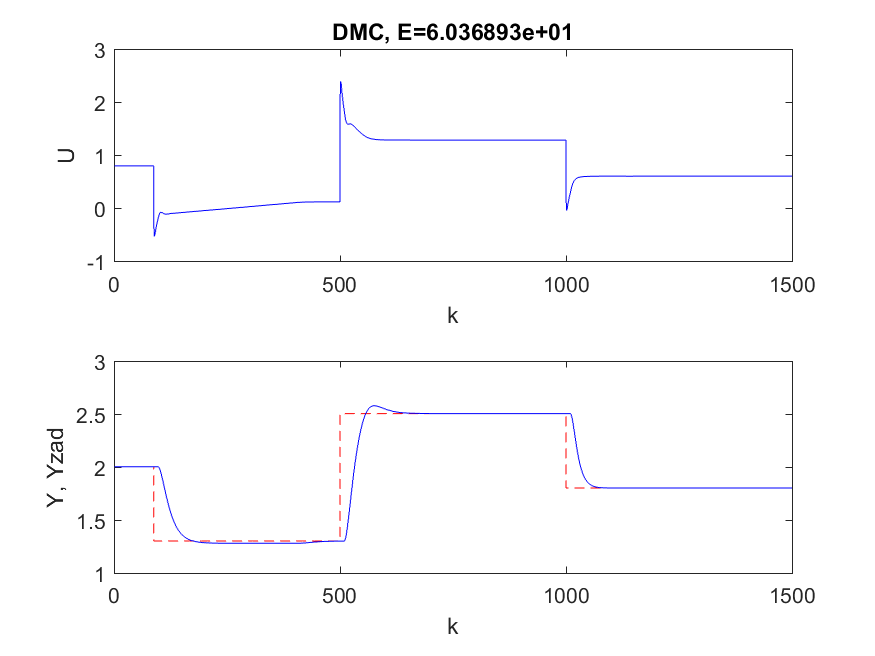
\includegraphics{dmc_optimized.png}
		\label{dmcopt}
\end{figure}